% !TEX TS-program = pdflatexmk
% !BIB program = biber
\documentclass[12pt]{../njit_thesis}
% Master file of the sample dissertation, which is also the guide to the
% template. It uses the class file, packages.tex, macros.tex, and the
% citation styles in the folder above, the same ones the starter document
% there uses. (LaTeX warns that "../njit_thesis" provides "njit_thesis";
% the warning is harmless.) Start your own thesis from ../main.tex, not
% from this file.

% ----------------------------------------------------------------------
% Package Imports and Macros
% ----------------------------------------------------------------------
% !TeX root = main.tex

% Table and alignment packages
\usepackage{tabularx}
\usepackage{booktabs}
\usepackage{array}

% Math packages
\usepackage{amsmath,amsfonts,amssymb,amsthm,mathtools}

% Graphics and subfigures
\usepackage{graphicx}
\usepackage{subcaption}

% URL breaking for references and tables
\usepackage{xurl}

% Quotations
\usepackage{csquotes}
\MakeOuterQuote{"}

%% Bibliography (BibLaTeX with Biber backend)
\usepackage[backend=biber,doi=false,url=false,defernums=true,sortcites=true]{biblatex}

\defbibheading{subbibliography}[\refname]{%
	{\normalfont\large\bfseries}%
}

\addbibresource{references.bib}
% !TEX root = main.tex
% MACROS AND THEOREM ENVIRONMENTS (included via % !TEX root = main.tex
% MACROS AND THEOREM ENVIRONMENTS (included via % !TEX root = main.tex
% MACROS AND THEOREM ENVIRONMENTS (included via \input{macros} in main.tex)
%
% Define your own notation here with \newcommand, so each symbol is typed the
% same way everywhere and can be changed in one place. Add new theorem-like
% environments here too; they share one counter and are numbered by chapter
% (Theorem 2.1, Lemma 2.2, ...).

% Mathematical blackboard bold shortcuts
\newcommand{\CC}{\mathbb{C}}
\newcommand{\RR}{\mathbb{R}}
\newcommand{\ZZ}{\mathbb{Z}}
\newcommand{\NN}{\mathbb{N}}
\newcommand{\QQ}{\mathbb{Q}}

% Trademark sign after a brand name: MATLAB\trademark
\newcommand{\trademark}{\textsuperscript{\texttrademark}}

% Standard BibTeX logo
\DeclareRobustCommand{\BibTeX}{%
  {\normalfont B\kern-.05em{\scshape i\kern-.025em b}\kern-.08em \TeX}%
}

% Standard Theorem Environments (via amsthm)
\theoremstyle{plain}
\newtheorem{theorem}{Theorem}[chapter]
\newtheorem{lemma}[theorem]{Lemma}
\newtheorem{proposition}[theorem]{Proposition}
\newtheorem{corollary}[theorem]{Corollary}

\theoremstyle{definition}
\newtheorem{definition}[theorem]{Definition}
\newtheorem{example}[theorem]{Example}

\theoremstyle{remark}
\newtheorem{remark}[theorem]{Remark}
 in main.tex)
%
% Define your own notation here with \newcommand, so each symbol is typed the
% same way everywhere and can be changed in one place. Add new theorem-like
% environments here too; they share one counter and are numbered by chapter
% (Theorem 2.1, Lemma 2.2, ...).

% Mathematical blackboard bold shortcuts
\newcommand{\CC}{\mathbb{C}}
\newcommand{\RR}{\mathbb{R}}
\newcommand{\ZZ}{\mathbb{Z}}
\newcommand{\NN}{\mathbb{N}}
\newcommand{\QQ}{\mathbb{Q}}

% Trademark sign after a brand name: MATLAB\trademark
\newcommand{\trademark}{\textsuperscript{\texttrademark}}

% Standard BibTeX logo
\DeclareRobustCommand{\BibTeX}{%
  {\normalfont B\kern-.05em{\scshape i\kern-.025em b}\kern-.08em \TeX}%
}

% Standard Theorem Environments (via amsthm)
\theoremstyle{plain}
\newtheorem{theorem}{Theorem}[chapter]
\newtheorem{lemma}[theorem]{Lemma}
\newtheorem{proposition}[theorem]{Proposition}
\newtheorem{corollary}[theorem]{Corollary}

\theoremstyle{definition}
\newtheorem{definition}[theorem]{Definition}
\newtheorem{example}[theorem]{Example}

\theoremstyle{remark}
\newtheorem{remark}[theorem]{Remark}
 in main.tex)
%
% Define your own notation here with \newcommand, so each symbol is typed the
% same way everywhere and can be changed in one place. Add new theorem-like
% environments here too; they share one counter and are numbered by chapter
% (Theorem 2.1, Lemma 2.2, ...).

% Mathematical blackboard bold shortcuts
\newcommand{\CC}{\mathbb{C}}
\newcommand{\RR}{\mathbb{R}}
\newcommand{\ZZ}{\mathbb{Z}}
\newcommand{\NN}{\mathbb{N}}
\newcommand{\QQ}{\mathbb{Q}}

% Trademark sign after a brand name: MATLAB\trademark
\newcommand{\trademark}{\textsuperscript{\texttrademark}}

% Standard BibTeX logo
\DeclareRobustCommand{\BibTeX}{%
  {\normalfont B\kern-.05em{\scshape i\kern-.025em b}\kern-.08em \TeX}%
}

% Standard Theorem Environments (via amsthm)
\theoremstyle{plain}
\newtheorem{theorem}{Theorem}[chapter]
\newtheorem{lemma}[theorem]{Lemma}
\newtheorem{proposition}[theorem]{Proposition}
\newtheorem{corollary}[theorem]{Corollary}

\theoremstyle{definition}
\newtheorem{definition}[theorem]{Definition}
\newtheorem{example}[theorem]{Example}

\theoremstyle{remark}
\newtheorem{remark}[theorem]{Remark}


% Graphics directory
\graphicspath{{Graphics/}}

\begin{document}

%%%%%%%%%%%%%%%%%%%%%%%%%%%%%%%%%%%%%%%%%%%%%%%%%%%%%%%%%%%%%%
%  Front Matter Initialization Pages:
%       ABSTRACT PAGE       (abstract.tex)
%       TITLE PAGE          (created by class file)
%       COPYRIGHT PAGE      (created by class file)
%       APPROVAL PAGE       (approval.tex)
%       BIOGRAPHY PAGE      (biography.tex)
%       DEDICATION PAGE     (dedication.tex, optional)
%       ACKNOWLEDGMENT PAGE (acknowledgment.tex)
%%%%%%%%%%%%%%%%%%%%%%%%%%%%%%%%%%%%%%%%%%%%%%%%%%%%%%%%%%%%%%

% Your title, name, degrees, and graduation date are set in biography.tex;
% your advisor and committee in approval.tex.
\abstract{% !TEX root = main.tex
% ABSTRACT (included via \abstract{% !TEX root = main.tex
% ABSTRACT (included via \abstract{% !TEX root = main.tex
% ABSTRACT (included via \abstract{\input{abstract}} in main.tex)
%
% Put ONLY the text of the abstract here. The class prints the ABSTRACT
% heading, your title (from \title in biography.tex) and your name above it,
% so the title is guaranteed to match the title and approval pages.
%
% GSO rules:
% - At most one page for a master's thesis, two pages for a dissertation.
% - Write in the third person and describe what was actually done in the
%   research: the question, the methods, and the main results.
% - If you explain why the topic matters, keep it to one or two sentences.
% The class double-spaces the text and sets the first paragraph flush left;
% do not add \noindent or spacing commands.
%
% Your own abstract goes in ../abstract.tex.

This document is both a guide to preparing an NJIT thesis or dissertation in \LaTeX\ and a working example of one: every page you are reading was produced by this template.

The abstract is the first page of the document and carries no page number. The class file prints the heading, the title, and the author's name above it, so \texttt{abstract.tex} contains only the text of the abstract. The Graduate Studies Office (GSO) limits the abstract to one page for a master's thesis and two pages for a doctoral dissertation. It should be written in the third person and describe what was actually done in the research: the question, the methods, and the main results. Any explanation of why the topic is important should be kept to one or two sentences. The title printed here must match the title on the title page and approval page word for word; the template guarantees this because the title is set only once, with \verb+\title+ in \texttt{biography.tex}.
} in main.tex)
%
% Put ONLY the text of the abstract here. The class prints the ABSTRACT
% heading, your title (from \title in biography.tex) and your name above it,
% so the title is guaranteed to match the title and approval pages.
%
% GSO rules:
% - At most one page for a master's thesis, two pages for a dissertation.
% - Write in the third person and describe what was actually done in the
%   research: the question, the methods, and the main results.
% - If you explain why the topic matters, keep it to one or two sentences.
% The class double-spaces the text and sets the first paragraph flush left;
% do not add \noindent or spacing commands.
%
% Your own abstract goes in ../abstract.tex.

This document is both a guide to preparing an NJIT thesis or dissertation in \LaTeX\ and a working example of one: every page you are reading was produced by this template.

The abstract is the first page of the document and carries no page number. The class file prints the heading, the title, and the author's name above it, so \texttt{abstract.tex} contains only the text of the abstract. The Graduate Studies Office (GSO) limits the abstract to one page for a master's thesis and two pages for a doctoral dissertation. It should be written in the third person and describe what was actually done in the research: the question, the methods, and the main results. Any explanation of why the topic is important should be kept to one or two sentences. The title printed here must match the title on the title page and approval page word for word; the template guarantees this because the title is set only once, with \verb+\title+ in \texttt{biography.tex}.
} in main.tex)
%
% Put ONLY the text of the abstract here. The class prints the ABSTRACT
% heading, your title (from \title in biography.tex) and your name above it,
% so the title is guaranteed to match the title and approval pages.
%
% GSO rules:
% - At most one page for a master's thesis, two pages for a dissertation.
% - Write in the third person and describe what was actually done in the
%   research: the question, the methods, and the main results.
% - If you explain why the topic matters, keep it to one or two sentences.
% The class double-spaces the text and sets the first paragraph flush left;
% do not add \noindent or spacing commands.
%
% Your own abstract goes in ../abstract.tex.

This document is both a guide to preparing an NJIT thesis or dissertation in \LaTeX\ and a working example of one: every page you are reading was produced by this template.

The abstract is the first page of the document and carries no page number. The class file prints the heading, the title, and the author's name above it, so \texttt{abstract.tex} contains only the text of the abstract. The Graduate Studies Office (GSO) limits the abstract to one page for a master's thesis and two pages for a doctoral dissertation. It should be written in the third person and describe what was actually done in the research: the question, the methods, and the main results. Any explanation of why the topic is important should be kept to one or two sentences. The title printed here must match the title on the title page and approval page word for word; the template guarantees this because the title is set only once, with \verb+\title+ in \texttt{biography.tex}.
}
% !TEX root = main.tex
% APPROVAL PAGE (included via % !TEX root = main.tex
% APPROVAL PAGE (included via % !TEX root = main.tex
% APPROVAL PAGE (included via \input{approval} in main.tex)
%
% \advisor{Name}{Title, Institution}  your advisor (listed first)
% \coadvisor{Name}{Title, Institution} optional; use once per co-advisor.
%                                     Co-advisors are listed right after
%                                     the advisor, and the advisor's line
%                                     then also reads "Co-advisor".
% \member{Name}{Title, Institution}   one line per committee member
%
% GSO rules:
% - A Ph.D. committee has at least five members; a master's committee at
%   least three.
% - List members from outside NJIT LAST, with their institution, city, and
%   state, with the state abbreviated as the Postal Service does (NJ).
% - Spell every name exactly as the person writes it, and copy each title
%   ("Associate Professor of ...") from the faculty directory in the current
%   Graduate Catalog. Wrong titles are a common reason for returned documents.
% - Write "Dr.\ Name" with the backslash so LaTeX does not add a
%   sentence-ending space after the period.
% With the thesis class option, "Dissertation Advisor" becomes "Thesis Advisor".

\advisor{Dr.\ Ellen M. Pawlikowski}
        {Professor of Chemical and Materials Engineering, NJIT}

% Uncomment if you have a co-advisor:
%\coadvisor{Dr.\ Firstname Lastname}
%          {Associate Professor of Chemical and Materials Engineering, NJIT}

\member{Dr.\ Nadine Aubry}
       {Distinguished Professor of Chemical and Materials Engineering, NJIT}

\member{Dr.\ Norma Clayton}
       {Associate Professor of Chemical and Materials Engineering, NJIT}

\member{Dr.\ Marjorie Perry}
       {Associate Professor of Chemical and Materials Engineering, NJIT}

\member{Dr.\ Virginia Sulzberger}
       {Director of Engineering, North American Electric Reliability Council, Princeton, NJ}
 in main.tex)
%
% \advisor{Name}{Title, Institution}  your advisor (listed first)
% \coadvisor{Name}{Title, Institution} optional; use once per co-advisor.
%                                     Co-advisors are listed right after
%                                     the advisor, and the advisor's line
%                                     then also reads "Co-advisor".
% \member{Name}{Title, Institution}   one line per committee member
%
% GSO rules:
% - A Ph.D. committee has at least five members; a master's committee at
%   least three.
% - List members from outside NJIT LAST, with their institution, city, and
%   state, with the state abbreviated as the Postal Service does (NJ).
% - Spell every name exactly as the person writes it, and copy each title
%   ("Associate Professor of ...") from the faculty directory in the current
%   Graduate Catalog. Wrong titles are a common reason for returned documents.
% - Write "Dr.\ Name" with the backslash so LaTeX does not add a
%   sentence-ending space after the period.
% With the thesis class option, "Dissertation Advisor" becomes "Thesis Advisor".

\advisor{Dr.\ Ellen M. Pawlikowski}
        {Professor of Chemical and Materials Engineering, NJIT}

% Uncomment if you have a co-advisor:
%\coadvisor{Dr.\ Firstname Lastname}
%          {Associate Professor of Chemical and Materials Engineering, NJIT}

\member{Dr.\ Nadine Aubry}
       {Distinguished Professor of Chemical and Materials Engineering, NJIT}

\member{Dr.\ Norma Clayton}
       {Associate Professor of Chemical and Materials Engineering, NJIT}

\member{Dr.\ Marjorie Perry}
       {Associate Professor of Chemical and Materials Engineering, NJIT}

\member{Dr.\ Virginia Sulzberger}
       {Director of Engineering, North American Electric Reliability Council, Princeton, NJ}
 in main.tex)
%
% \advisor{Name}{Title, Institution}  your advisor (listed first)
% \coadvisor{Name}{Title, Institution} optional; use once per co-advisor.
%                                     Co-advisors are listed right after
%                                     the advisor, and the advisor's line
%                                     then also reads "Co-advisor".
% \member{Name}{Title, Institution}   one line per committee member
%
% GSO rules:
% - A Ph.D. committee has at least five members; a master's committee at
%   least three.
% - List members from outside NJIT LAST, with their institution, city, and
%   state, with the state abbreviated as the Postal Service does (NJ).
% - Spell every name exactly as the person writes it, and copy each title
%   ("Associate Professor of ...") from the faculty directory in the current
%   Graduate Catalog. Wrong titles are a common reason for returned documents.
% - Write "Dr.\ Name" with the backslash so LaTeX does not add a
%   sentence-ending space after the period.
% With the thesis class option, "Dissertation Advisor" becomes "Thesis Advisor".

\advisor{Dr.\ Ellen M. Pawlikowski}
        {Professor of Chemical and Materials Engineering, NJIT}

% Uncomment if you have a co-advisor:
%\coadvisor{Dr.\ Firstname Lastname}
%          {Associate Professor of Chemical and Materials Engineering, NJIT}

\member{Dr.\ Nadine Aubry}
       {Distinguished Professor of Chemical and Materials Engineering, NJIT}

\member{Dr.\ Norma Clayton}
       {Associate Professor of Chemical and Materials Engineering, NJIT}

\member{Dr.\ Marjorie Perry}
       {Associate Professor of Chemical and Materials Engineering, NJIT}

\member{Dr.\ Virginia Sulzberger}
       {Director of Engineering, North American Electric Reliability Council, Princeton, NJ}

% !TEX root = main.tex
% TITLE-PAGE AND BIOGRAPHICAL SKETCH INFORMATION
% (included via % !TEX root = main.tex
% TITLE-PAGE AND BIOGRAPHICAL SKETCH INFORMATION
% (included via % !TEX root = main.tex
% TITLE-PAGE AND BIOGRAPHICAL SKETCH INFORMATION
% (included via \input{biography} in main.tex)
%
% Everything here is set ONCE and reused on the abstract, title, copyright,
% approval and biography pages, so the pages cannot disagree.
%
% \title           Type it in normal capitalization; the class sets it in
%                  capitals where the GSO requires.
% \author          Your name exactly as it should appear on the diploma.
% \graduationdate  Month (May, August or December) and year you GRADUATE,
%                  not the date you defend.
% \thisdegree      Full name of the degree you are receiving.
% \degreeearned    One line per degree earned, MOST RECENT FIRST, starting
%                  with the degree you are receiving now:
%                  \degreeearned{Degree name}{University, City, State, Year}.
%                  Use the exact degree title from your transcript.
% \degreelevel     Optional. Overrides the "Degree:" line of the sketch,
%                  which defaults to "Doctor of Philosophy" (or "Master of
%                  Science" with the thesis class option).
%
% For a master's thesis, use \documentclass[12pt,thesis]{njit_thesis} in
% main.tex: the title page says "A Thesis" and the copyright page is blank.
%
% Presentations and publications are listed automatically from
% references.bib, newest first: add  keywords = {me}  to each of your own
% entries. Papers in preparation, submitted or under review may be included.

\title{Writing your NJIT dissertation: a sample and guide}

\author{Charles C.\ Highlander}

\major{Chemical Engineering}

% Month (May, August or December) and year you GRADUATE
\graduationdate{May}{2026}

\thisdegree{Doctor of Philosophy in Chemical Engineering}
\department{Otto H.\ York Department of Chemical and Materials Engineering}

%% Uncomment one of the following two institutes
%% For departments/degrees at NJIT
\institute{New Jersey Institute of Technology}
%% For departments/degrees joint with RU-Newark (including the math department)
% \institute{New Jersey Institute of Technology and \par Rutgers, The State University of New Jersey---Newark}
  
% List degrees with most recent first, that is the current degree you are
% about to graduate with (examples are given after the general format)


\degreeearned{Doctor of Philosophy in Chemical Engineering}{New Jersey Institute of Technology, Newark, NJ, 2026}

\degreeearned{Master of Science in Chemical Engineering}{New Jersey Institute of Technology, Newark, NJ, 2020}
       
\degreeearned{Bachelor of Science in Chemical Engineering}
       {New Jersey Institute of Technology, Newark, NJ, 2018}
       


% If you don't have any publications uncomment below
%\renewcommand{\printmypublications}{}


  in main.tex)
%
% Everything here is set ONCE and reused on the abstract, title, copyright,
% approval and biography pages, so the pages cannot disagree.
%
% \title           Type it in normal capitalization; the class sets it in
%                  capitals where the GSO requires.
% \author          Your name exactly as it should appear on the diploma.
% \graduationdate  Month (May, August or December) and year you GRADUATE,
%                  not the date you defend.
% \thisdegree      Full name of the degree you are receiving.
% \degreeearned    One line per degree earned, MOST RECENT FIRST, starting
%                  with the degree you are receiving now:
%                  \degreeearned{Degree name}{University, City, State, Year}.
%                  Use the exact degree title from your transcript.
% \degreelevel     Optional. Overrides the "Degree:" line of the sketch,
%                  which defaults to "Doctor of Philosophy" (or "Master of
%                  Science" with the thesis class option).
%
% For a master's thesis, use \documentclass[12pt,thesis]{njit_thesis} in
% main.tex: the title page says "A Thesis" and the copyright page is blank.
%
% Presentations and publications are listed automatically from
% references.bib, newest first: add  keywords = {me}  to each of your own
% entries. Papers in preparation, submitted or under review may be included.

\title{Writing your NJIT dissertation: a sample and guide}

\author{Charles C.\ Highlander}

\major{Chemical Engineering}

% Month (May, August or December) and year you GRADUATE
\graduationdate{May}{2026}

\thisdegree{Doctor of Philosophy in Chemical Engineering}
\department{Otto H.\ York Department of Chemical and Materials Engineering}

%% Uncomment one of the following two institutes
%% For departments/degrees at NJIT
\institute{New Jersey Institute of Technology}
%% For departments/degrees joint with RU-Newark (including the math department)
% \institute{New Jersey Institute of Technology and \par Rutgers, The State University of New Jersey---Newark}
  
% List degrees with most recent first, that is the current degree you are
% about to graduate with (examples are given after the general format)


\degreeearned{Doctor of Philosophy in Chemical Engineering}{New Jersey Institute of Technology, Newark, NJ, 2026}

\degreeearned{Master of Science in Chemical Engineering}{New Jersey Institute of Technology, Newark, NJ, 2020}
       
\degreeearned{Bachelor of Science in Chemical Engineering}
       {New Jersey Institute of Technology, Newark, NJ, 2018}
       


% If you don't have any publications uncomment below
%\renewcommand{\printmypublications}{}


  in main.tex)
%
% Everything here is set ONCE and reused on the abstract, title, copyright,
% approval and biography pages, so the pages cannot disagree.
%
% \title           Type it in normal capitalization; the class sets it in
%                  capitals where the GSO requires.
% \author          Your name exactly as it should appear on the diploma.
% \graduationdate  Month (May, August or December) and year you GRADUATE,
%                  not the date you defend.
% \thisdegree      Full name of the degree you are receiving.
% \degreeearned    One line per degree earned, MOST RECENT FIRST, starting
%                  with the degree you are receiving now:
%                  \degreeearned{Degree name}{University, City, State, Year}.
%                  Use the exact degree title from your transcript.
% \degreelevel     Optional. Overrides the "Degree:" line of the sketch,
%                  which defaults to "Doctor of Philosophy" (or "Master of
%                  Science" with the thesis class option).
%
% For a master's thesis, use \documentclass[12pt,thesis]{njit_thesis} in
% main.tex: the title page says "A Thesis" and the copyright page is blank.
%
% Presentations and publications are listed automatically from
% references.bib, newest first: add  keywords = {me}  to each of your own
% entries. Papers in preparation, submitted or under review may be included.

\title{Writing your NJIT dissertation: a sample and guide}

\author{Charles C.\ Highlander}

\major{Chemical Engineering}

% Month (May, August or December) and year you GRADUATE
\graduationdate{May}{2026}

\thisdegree{Doctor of Philosophy in Chemical Engineering}
\department{Otto H.\ York Department of Chemical and Materials Engineering}

%% Uncomment one of the following two institutes
%% For departments/degrees at NJIT
\institute{New Jersey Institute of Technology}
%% For departments/degrees joint with RU-Newark (including the math department)
% \institute{New Jersey Institute of Technology and \par Rutgers, The State University of New Jersey---Newark}
  
% List degrees with most recent first, that is the current degree you are
% about to graduate with (examples are given after the general format)


\degreeearned{Doctor of Philosophy in Chemical Engineering}{New Jersey Institute of Technology, Newark, NJ, 2026}

\degreeearned{Master of Science in Chemical Engineering}{New Jersey Institute of Technology, Newark, NJ, 2020}
       
\degreeearned{Bachelor of Science in Chemical Engineering}
       {New Jersey Institute of Technology, Newark, NJ, 2018}
       


% If you don't have any publications uncomment below
%\renewcommand{\printmypublications}{}


 
\dedication{% !TEX root = main.tex
% DEDICATION (optional; included via \dedication{% !TEX root = main.tex
% DEDICATION (optional; included via \dedication{% !TEX root = main.tex
% DEDICATION (optional; included via \dedication{\input{dedication}} in main.tex)
%
% A short dedication or quotation, set single-spaced in a centered block.
% Check the spelling of names and keep person and tense consistent (GSO).
% To omit the page, comment out the \dedication line in main.tex.
% Words left out of a quotation are marked with an ellipsis, typed \ldots;
% between two full sentences the first keeps its period (Chicago style).

\emph{Power of concentration is a very valuable quality, which few people acquire except through education. \ldots{} To be able to concentrate on the same matter for a considerable time is essential to difficult achievement, and even to the understanding of any complicated or abstruse subject.}

\begin{flushright}
Bertrand Russell, \emph{On Education} (1926)
\end{flushright}
} in main.tex)
%
% A short dedication or quotation, set single-spaced in a centered block.
% Check the spelling of names and keep person and tense consistent (GSO).
% To omit the page, comment out the \dedication line in main.tex.
% Words left out of a quotation are marked with an ellipsis, typed \ldots;
% between two full sentences the first keeps its period (Chicago style).

\emph{Power of concentration is a very valuable quality, which few people acquire except through education. \ldots{} To be able to concentrate on the same matter for a considerable time is essential to difficult achievement, and even to the understanding of any complicated or abstruse subject.}

\begin{flushright}
Bertrand Russell, \emph{On Education} (1926)
\end{flushright}
} in main.tex)
%
% A short dedication or quotation, set single-spaced in a centered block.
% Check the spelling of names and keep person and tense consistent (GSO).
% To omit the page, comment out the \dedication line in main.tex.
% Words left out of a quotation are marked with an ellipsis, typed \ldots;
% between two full sentences the first keeps its period (Chicago style).

\emph{Power of concentration is a very valuable quality, which few people acquire except through education. \ldots{} To be able to concentrate on the same matter for a considerable time is essential to difficult achievement, and even to the understanding of any complicated or abstruse subject.}

\begin{flushright}
Bertrand Russell, \emph{On Education} (1926)
\end{flushright}
}
\acknowledgment{% !TEX root = main.tex

% ACKNOWLEDGMENTS (included via \acknowledgment{% !TEX root = main.tex

% ACKNOWLEDGMENTS (included via \acknowledgment{% !TEX root = main.tex

% ACKNOWLEDGMENTS (included via \acknowledgment{\input{acknowledgment}} in main.tex)
%
% Write ordinary paragraphs; the class prints the heading, double-spaces the
% text, and sets the first paragraph flush left. Do not use \noindent.
%
% GSO order: your ADVISOR first, then your COMMITTEE. The 2025 GSO Front
% Matter guide then lists other contributors and peers, family, funding
% sources, and technical support. Acknowledge each grant by agency and grant
% number; many funders require it.

% First thank the advisor
Many thanks to my Advisor, Dr.\ Ellen M.\ Pawlikowski, for her guidance, patience, and encouragement throughout my doctoral studies.

% Then thank the committee
My Committee Members, Drs.\ Nadine Aubry, Norma Clayton, and Marjorie Perry, were very generous with their time and advice. Special thanks to my external committee member, Dr.\ Virginia Sulzberger, for bringing her experience at the North American Electric Reliability Council to my committee.

% Then acknowledge financial support
I gratefully acknowledge support from the National Science Foundation under grant CBET-0000000.

% Then thank for technical support
I thank NJIT Academic and Research Computing Systems for keeping the computing cluster running and for their help whenever my simulations would not. Many long days of work were fueled by the campus coffee shop, where Miss Jackie always had a friendly word and a fresh cup. She is missed.

% Finally friends and family
I would like to thank the students and faculty of the NJIT Department of Mathematical Sciences who built and improved this \LaTeX\ template: Adrienne C.\ N.\ James, who created the first edition with Jerry Jen-Sou Chen; Eliana Antoniou, Stephen A.\ Kunec, Hoa Kien Tran, and Shoubhik Mondal, who revised it; and Jimmie Adriazola, Prof.\ Roy Goodman, and Prof.\ Christina Frederick, who revised it further, with help from Claude.ai. Ester Flaim of the Graduate Studies Office contributed to and edited this latest revision. Thanks also to everyone else who contributed along the way. Their work does a great job of laying out my dissertation, so I can spend more time on improving the content.
} in main.tex)
%
% Write ordinary paragraphs; the class prints the heading, double-spaces the
% text, and sets the first paragraph flush left. Do not use \noindent.
%
% GSO order: your ADVISOR first, then your COMMITTEE. The 2025 GSO Front
% Matter guide then lists other contributors and peers, family, funding
% sources, and technical support. Acknowledge each grant by agency and grant
% number; many funders require it.

% First thank the advisor
Many thanks to my Advisor, Dr.\ Ellen M.\ Pawlikowski, for her guidance, patience, and encouragement throughout my doctoral studies.

% Then thank the committee
My Committee Members, Drs.\ Nadine Aubry, Norma Clayton, and Marjorie Perry, were very generous with their time and advice. Special thanks to my external committee member, Dr.\ Virginia Sulzberger, for bringing her experience at the North American Electric Reliability Council to my committee.

% Then acknowledge financial support
I gratefully acknowledge support from the National Science Foundation under grant CBET-0000000.

% Then thank for technical support
I thank NJIT Academic and Research Computing Systems for keeping the computing cluster running and for their help whenever my simulations would not. Many long days of work were fueled by the campus coffee shop, where Miss Jackie always had a friendly word and a fresh cup. She is missed.

% Finally friends and family
I would like to thank the students and faculty of the NJIT Department of Mathematical Sciences who built and improved this \LaTeX\ template: Adrienne C.\ N.\ James, who created the first edition with Jerry Jen-Sou Chen; Eliana Antoniou, Stephen A.\ Kunec, Hoa Kien Tran, and Shoubhik Mondal, who revised it; and Jimmie Adriazola, Prof.\ Roy Goodman, and Prof.\ Christina Frederick, who revised it further, with help from Claude.ai. Ester Flaim of the Graduate Studies Office contributed to and edited this latest revision. Thanks also to everyone else who contributed along the way. Their work does a great job of laying out my dissertation, so I can spend more time on improving the content.
} in main.tex)
%
% Write ordinary paragraphs; the class prints the heading, double-spaces the
% text, and sets the first paragraph flush left. Do not use \noindent.
%
% GSO order: your ADVISOR first, then your COMMITTEE. The 2025 GSO Front
% Matter guide then lists other contributors and peers, family, funding
% sources, and technical support. Acknowledge each grant by agency and grant
% number; many funders require it.

% First thank the advisor
Many thanks to my Advisor, Dr.\ Ellen M.\ Pawlikowski, for her guidance, patience, and encouragement throughout my doctoral studies.

% Then thank the committee
My Committee Members, Drs.\ Nadine Aubry, Norma Clayton, and Marjorie Perry, were very generous with their time and advice. Special thanks to my external committee member, Dr.\ Virginia Sulzberger, for bringing her experience at the North American Electric Reliability Council to my committee.

% Then acknowledge financial support
I gratefully acknowledge support from the National Science Foundation under grant CBET-0000000.

% Then thank for technical support
I thank NJIT Academic and Research Computing Systems for keeping the computing cluster running and for their help whenever my simulations would not. Many long days of work were fueled by the campus coffee shop, where Miss Jackie always had a friendly word and a fresh cup. She is missed.

% Finally friends and family
I would like to thank the students and faculty of the NJIT Department of Mathematical Sciences who built and improved this \LaTeX\ template: Adrienne C.\ N.\ James, who created the first edition with Jerry Jen-Sou Chen; Eliana Antoniou, Stephen A.\ Kunec, Hoa Kien Tran, and Shoubhik Mondal, who revised it; and Jimmie Adriazola, Prof.\ Roy Goodman, and Prof.\ Christina Frederick, who revised it further, with help from Claude.ai. Ester Flaim of the Graduate Studies Office contributed to and edited this latest revision. Thanks also to everyone else who contributed along the way. Their work does a great job of laying out my dissertation, so I can spend more time on improving the content.
}

% Optional preliminary lists data
\symbols{% !TEX root = main.tex
% List of Symbols (included via \symbols{% !TEX root = main.tex
% List of Symbols (included via \symbols{% !TEX root = main.tex
% List of Symbols (included via \symbols{\input{listofsymbols}} in main.tex)
%
% A two-column table: the symbol, then its description. Start each
% description with a capital letter and write it in sentence case (GSO).
% Organize the list by category or function, alphabetically by name, or by
% frequency of use (GSO). Alphabetical order follows the characters
% themselves, so * comes after &. The sample is organized by category.
% The table continues across pages automatically. To widen the symbol
% column, give a width: \begin{symboltable}[1.5in]

\begin{symboltable}
% Number systems
\sym{$\ZZ$}{The ring of integers}
\sym{$\RR$}{The field of real numbers}
\sym{$\CC$}{The field of complex numbers}
% Spaces and groups
\sym{$H^1(\RR)$}{The Sobolev space of functions over $\RR$ that are square-integrable and whose weak first derivative is square-integrable}
\sym{$\mathrm{GL}_2(\RR)$}{The general linear group of real invertible $2\times 2$ matrices}
% Physical quantities
\sym{$c$}{Speed of light in vacuum ($c \approx 3 \times 10^8\text{ m/s}$)}
\sym{$E$}{Energy of a physical system}
\sym{$m$}{Mass of a physical body}
% Other notation
\sym{$\%$}{Percentage sign}
\end{symboltable}
} in main.tex)
%
% A two-column table: the symbol, then its description. Start each
% description with a capital letter and write it in sentence case (GSO).
% Organize the list by category or function, alphabetically by name, or by
% frequency of use (GSO). Alphabetical order follows the characters
% themselves, so * comes after &. The sample is organized by category.
% The table continues across pages automatically. To widen the symbol
% column, give a width: \begin{symboltable}[1.5in]

\begin{symboltable}
% Number systems
\sym{$\ZZ$}{The ring of integers}
\sym{$\RR$}{The field of real numbers}
\sym{$\CC$}{The field of complex numbers}
% Spaces and groups
\sym{$H^1(\RR)$}{The Sobolev space of functions over $\RR$ that are square-integrable and whose weak first derivative is square-integrable}
\sym{$\mathrm{GL}_2(\RR)$}{The general linear group of real invertible $2\times 2$ matrices}
% Physical quantities
\sym{$c$}{Speed of light in vacuum ($c \approx 3 \times 10^8\text{ m/s}$)}
\sym{$E$}{Energy of a physical system}
\sym{$m$}{Mass of a physical body}
% Other notation
\sym{$\%$}{Percentage sign}
\end{symboltable}
} in main.tex)
%
% A two-column table: the symbol, then its description. Start each
% description with a capital letter and write it in sentence case (GSO).
% Organize the list by category or function, alphabetically by name, or by
% frequency of use (GSO). Alphabetical order follows the characters
% themselves, so * comes after &. The sample is organized by category.
% The table continues across pages automatically. To widen the symbol
% column, give a width: \begin{symboltable}[1.5in]

\begin{symboltable}
% Number systems
\sym{$\ZZ$}{The ring of integers}
\sym{$\RR$}{The field of real numbers}
\sym{$\CC$}{The field of complex numbers}
% Spaces and groups
\sym{$H^1(\RR)$}{The Sobolev space of functions over $\RR$ that are square-integrable and whose weak first derivative is square-integrable}
\sym{$\mathrm{GL}_2(\RR)$}{The general linear group of real invertible $2\times 2$ matrices}
% Physical quantities
\sym{$c$}{Speed of light in vacuum ($c \approx 3 \times 10^8\text{ m/s}$)}
\sym{$E$}{Energy of a physical system}
\sym{$m$}{Mass of a physical body}
% Other notation
\sym{$\%$}{Percentage sign}
\end{symboltable}
}
\glossaryofterms{% !TEX root = main.tex
% Glossary of Terms (included via \glossaryofterms{% !TEX root = main.tex
% Glossary of Terms (included via \glossaryofterms{% !TEX root = main.tex
% Glossary of Terms (included via \glossaryofterms{\input{listofdefinitions}} in main.tex)
%
% A two-column table: the term, then its definition. List terms in
% alphabetical order. Start each definition with a capital letter and write
% it in sentence case; capitalize only acronyms and proper names (GSO).
% The table continues across pages automatically. To change the width of
% the term column, give a width: \begin{glossarytable}[2in]
%
% Commands cannot be shown with \verb inside \term{...}, because each entry is
% an argument of \term; write \texttt{\textbackslash{}cite\{key\}} instead.

\begin{glossarytable}
\term{Argument}{Input given to a command in braces, as in \texttt{\textbackslash{}section\{Title\}}. Optional arguments go in square brackets, as in \texttt{\textbackslash{}includegraphics[width=3in]\{file\}}.}
\term{Auxiliary file}{A file such as \texttt{main.aux} or \texttt{main.toc} that \LaTeX\ writes during one run and reads on the next to resolve cross-references and lists. Deleting these files is a safe first step when a build behaves strangely.}
\term{Biber}{The program that reads \texttt{references.bib} and sorts and formats the bibliography for \texttt{biblatex}. It runs between \LaTeX\ runs.}
\term{\texttt{biblatex}}{The package that formats citations and the bibliography. The citation style is chosen once, in \texttt{packages.tex}.}
\term{\BibTeX\ entry}{One record in a \texttt{.bib} file, such as \texttt{@article\{key, ...\}}. The key is the name used in \texttt{\textbackslash{}cite\{key\}}.}
\term{Class file}{A file ending in \texttt{.cls} that defines a document's overall layout. This template's class, \texttt{njit\_thesis.cls}, implements the NJIT formatting rules.}
\term{Command}{An instruction that begins with a backslash, such as \texttt{\textbackslash{}chapter} or \texttt{\textbackslash{}cite}.}
\term{Comment}{Text after a \texttt{\%} sign on a line. \LaTeX\ ignores it, so comments are useful for notes and for temporarily removing material.}
\term{Cross-reference}{A reference to a numbered item, made with \texttt{\textbackslash{}label} and \texttt{\textbackslash{}ref} (or \texttt{\textbackslash{}eqref} for equations). Numbers update automatically when material moves.}
\term{Environment}{A block of material between \texttt{\textbackslash{}begin\{name\}} and \texttt{\textbackslash{}end\{name\}}, such as \texttt{figure}, \texttt{table}, or \texttt{equation}.}
\term{Float}{A figure or table that \LaTeX\ may move to a nearby page to avoid large gaps. Always refer to floats by number, not as ``the figure below.''}
\term{Label}{A name attached to a numbered item with \texttt{\textbackslash{}label\{name\}}, so it can be referred to with \texttt{\textbackslash{}ref\{name\}}. Prefixes such as \texttt{fig:} or \texttt{eq:} keep labels organized.}
\term{\texttt{latexmk}}{A program that runs \LaTeX\ and Biber as many times as needed to produce a complete document. Running \texttt{latexmk -pdf main.tex} builds this thesis.}
\term{Log file}{The file \texttt{main.log}, which records every warning and error from a run. Check it for undefined references and overfull boxes before submitting.}
\term{Macro}{A command you define yourself with \texttt{\textbackslash{}newcommand}, usually in \texttt{macros.tex}, to keep notation consistent and save typing.}
\term{Overfull box}{A warning that a line or object is too wide and sticks into the margin. The GSO checks margins, so fix these by rewording, adding a hyphenation point, or resizing the object.}
\term{Overleaf}{A website for editing and compiling \LaTeX\ documents in a browser, with no local installation.}
\term{Package}{A file loaded with \texttt{\textbackslash{}usepackage} that adds features, such as \texttt{amsmath} for mathematics or \texttt{graphicx} for images. This template loads its packages in \texttt{packages.tex}.}
\term{Preamble}{Everything in \texttt{main.tex} before \texttt{\textbackslash{}begin\{document\}}, where the class, packages, and macros are loaded.}
\term{Undefined reference}{A \texttt{\textbackslash{}ref} or \texttt{\textbackslash{}cite} that \LaTeX\ cannot resolve, shown as ``??'' in the PDF. It usually means a misspelled label or citation key, or that the document needs another run.}
\end{glossarytable}
} in main.tex)
%
% A two-column table: the term, then its definition. List terms in
% alphabetical order. Start each definition with a capital letter and write
% it in sentence case; capitalize only acronyms and proper names (GSO).
% The table continues across pages automatically. To change the width of
% the term column, give a width: \begin{glossarytable}[2in]
%
% Commands cannot be shown with \verb inside \term{...}, because each entry is
% an argument of \term; write \texttt{\textbackslash{}cite\{key\}} instead.

\begin{glossarytable}
\term{Argument}{Input given to a command in braces, as in \texttt{\textbackslash{}section\{Title\}}. Optional arguments go in square brackets, as in \texttt{\textbackslash{}includegraphics[width=3in]\{file\}}.}
\term{Auxiliary file}{A file such as \texttt{main.aux} or \texttt{main.toc} that \LaTeX\ writes during one run and reads on the next to resolve cross-references and lists. Deleting these files is a safe first step when a build behaves strangely.}
\term{Biber}{The program that reads \texttt{references.bib} and sorts and formats the bibliography for \texttt{biblatex}. It runs between \LaTeX\ runs.}
\term{\texttt{biblatex}}{The package that formats citations and the bibliography. The citation style is chosen once, in \texttt{packages.tex}.}
\term{\BibTeX\ entry}{One record in a \texttt{.bib} file, such as \texttt{@article\{key, ...\}}. The key is the name used in \texttt{\textbackslash{}cite\{key\}}.}
\term{Class file}{A file ending in \texttt{.cls} that defines a document's overall layout. This template's class, \texttt{njit\_thesis.cls}, implements the NJIT formatting rules.}
\term{Command}{An instruction that begins with a backslash, such as \texttt{\textbackslash{}chapter} or \texttt{\textbackslash{}cite}.}
\term{Comment}{Text after a \texttt{\%} sign on a line. \LaTeX\ ignores it, so comments are useful for notes and for temporarily removing material.}
\term{Cross-reference}{A reference to a numbered item, made with \texttt{\textbackslash{}label} and \texttt{\textbackslash{}ref} (or \texttt{\textbackslash{}eqref} for equations). Numbers update automatically when material moves.}
\term{Environment}{A block of material between \texttt{\textbackslash{}begin\{name\}} and \texttt{\textbackslash{}end\{name\}}, such as \texttt{figure}, \texttt{table}, or \texttt{equation}.}
\term{Float}{A figure or table that \LaTeX\ may move to a nearby page to avoid large gaps. Always refer to floats by number, not as ``the figure below.''}
\term{Label}{A name attached to a numbered item with \texttt{\textbackslash{}label\{name\}}, so it can be referred to with \texttt{\textbackslash{}ref\{name\}}. Prefixes such as \texttt{fig:} or \texttt{eq:} keep labels organized.}
\term{\texttt{latexmk}}{A program that runs \LaTeX\ and Biber as many times as needed to produce a complete document. Running \texttt{latexmk -pdf main.tex} builds this thesis.}
\term{Log file}{The file \texttt{main.log}, which records every warning and error from a run. Check it for undefined references and overfull boxes before submitting.}
\term{Macro}{A command you define yourself with \texttt{\textbackslash{}newcommand}, usually in \texttt{macros.tex}, to keep notation consistent and save typing.}
\term{Overfull box}{A warning that a line or object is too wide and sticks into the margin. The GSO checks margins, so fix these by rewording, adding a hyphenation point, or resizing the object.}
\term{Overleaf}{A website for editing and compiling \LaTeX\ documents in a browser, with no local installation.}
\term{Package}{A file loaded with \texttt{\textbackslash{}usepackage} that adds features, such as \texttt{amsmath} for mathematics or \texttt{graphicx} for images. This template loads its packages in \texttt{packages.tex}.}
\term{Preamble}{Everything in \texttt{main.tex} before \texttt{\textbackslash{}begin\{document\}}, where the class, packages, and macros are loaded.}
\term{Undefined reference}{A \texttt{\textbackslash{}ref} or \texttt{\textbackslash{}cite} that \LaTeX\ cannot resolve, shown as ``??'' in the PDF. It usually means a misspelled label or citation key, or that the document needs another run.}
\end{glossarytable}
} in main.tex)
%
% A two-column table: the term, then its definition. List terms in
% alphabetical order. Start each definition with a capital letter and write
% it in sentence case; capitalize only acronyms and proper names (GSO).
% The table continues across pages automatically. To change the width of
% the term column, give a width: \begin{glossarytable}[2in]
%
% Commands cannot be shown with \verb inside \term{...}, because each entry is
% an argument of \term; write \texttt{\textbackslash{}cite\{key\}} instead.

\begin{glossarytable}
\term{Argument}{Input given to a command in braces, as in \texttt{\textbackslash{}section\{Title\}}. Optional arguments go in square brackets, as in \texttt{\textbackslash{}includegraphics[width=3in]\{file\}}.}
\term{Auxiliary file}{A file such as \texttt{main.aux} or \texttt{main.toc} that \LaTeX\ writes during one run and reads on the next to resolve cross-references and lists. Deleting these files is a safe first step when a build behaves strangely.}
\term{Biber}{The program that reads \texttt{references.bib} and sorts and formats the bibliography for \texttt{biblatex}. It runs between \LaTeX\ runs.}
\term{\texttt{biblatex}}{The package that formats citations and the bibliography. The citation style is chosen once, in \texttt{packages.tex}.}
\term{\BibTeX\ entry}{One record in a \texttt{.bib} file, such as \texttt{@article\{key, ...\}}. The key is the name used in \texttt{\textbackslash{}cite\{key\}}.}
\term{Class file}{A file ending in \texttt{.cls} that defines a document's overall layout. This template's class, \texttt{njit\_thesis.cls}, implements the NJIT formatting rules.}
\term{Command}{An instruction that begins with a backslash, such as \texttt{\textbackslash{}chapter} or \texttt{\textbackslash{}cite}.}
\term{Comment}{Text after a \texttt{\%} sign on a line. \LaTeX\ ignores it, so comments are useful for notes and for temporarily removing material.}
\term{Cross-reference}{A reference to a numbered item, made with \texttt{\textbackslash{}label} and \texttt{\textbackslash{}ref} (or \texttt{\textbackslash{}eqref} for equations). Numbers update automatically when material moves.}
\term{Environment}{A block of material between \texttt{\textbackslash{}begin\{name\}} and \texttt{\textbackslash{}end\{name\}}, such as \texttt{figure}, \texttt{table}, or \texttt{equation}.}
\term{Float}{A figure or table that \LaTeX\ may move to a nearby page to avoid large gaps. Always refer to floats by number, not as ``the figure below.''}
\term{Label}{A name attached to a numbered item with \texttt{\textbackslash{}label\{name\}}, so it can be referred to with \texttt{\textbackslash{}ref\{name\}}. Prefixes such as \texttt{fig:} or \texttt{eq:} keep labels organized.}
\term{\texttt{latexmk}}{A program that runs \LaTeX\ and Biber as many times as needed to produce a complete document. Running \texttt{latexmk -pdf main.tex} builds this thesis.}
\term{Log file}{The file \texttt{main.log}, which records every warning and error from a run. Check it for undefined references and overfull boxes before submitting.}
\term{Macro}{A command you define yourself with \texttt{\textbackslash{}newcommand}, usually in \texttt{macros.tex}, to keep notation consistent and save typing.}
\term{Overfull box}{A warning that a line or object is too wide and sticks into the margin. The GSO checks margins, so fix these by rewording, adding a hyphenation point, or resizing the object.}
\term{Overleaf}{A website for editing and compiling \LaTeX\ documents in a browser, with no local installation.}
\term{Package}{A file loaded with \texttt{\textbackslash{}usepackage} that adds features, such as \texttt{amsmath} for mathematics or \texttt{graphicx} for images. This template loads its packages in \texttt{packages.tex}.}
\term{Preamble}{Everything in \texttt{main.tex} before \texttt{\textbackslash{}begin\{document\}}, where the class, packages, and macros are loaded.}
\term{Undefined reference}{A \texttt{\textbackslash{}ref} or \texttt{\textbackslash{}cite} that \LaTeX\ cannot resolve, shown as ``??'' in the PDF. It usually means a misspelled label or citation key, or that the document needs another run.}
\end{glossarytable}
}

% Generate all front matter pages in NJIT prescribed order
\initthesis

%%%%%%%%%%%%%%%%%%%%%%%%%%%%%%%%%%%%%%%%%%%%%%%%%%%%%%
%  Table of Contents and Preliminary Lists:
%       TABLE OF CONTENTS
%       LIST OF TABLES
%       LIST OF FIGURES
%       LIST OF SYMBOLS (optional)
%       GLOSSARY OF TERMS (optional)
%%%%%%%%%%%%%%%%%%%%%%%%%%%%%%%%%%%%%%%%%%%%%%%%%%%%%%
% The titles in the Table of Contents and the Lists of Tables and Figures must
% match the headings and captions in the text EXACTLY, word for word and in
% capitalization (GSO). Do not use the optional short forms
% \caption[short]{long} or \section[short]{long}.
\tableofcontents
\listoftables
\listoffigures
\listofalgorithms % comment out if you have no algorithms
\makelistofsymbols % comment out if you have no symbols
\makeglossaryofterms % comment out if you have no glossary

%%%%%%%%%%%%%%%%%%%%%%%%%%%%%%%%%%%%%%%%%%%%%%%%%%%%%%
%% START MAIN BODY OF THESIS
%% Arabic page numbering (1, 2, 3...) begins here
%%%%%%%%%%%%%%%%%%%%%%%%%%%%%%%%%%%%%%%%%%%%%%%%%%%%%%
\startbody


% Dissertation Chapters
% !TEX root = main.tex
% Chapter 1: what to do first, the files you edit, how to compile, and what
% to do when compiling fails.
%
% Each chapter lives in its own file, included from main.tex with \input.
% Start the file with \chapter{Title}; type the title in normal
% capitalization (the class sets it in capitals). Headings below it:
%   \section       level 2, Title Case
%   \subsection    level 3, sentence case
%   \subsubsection level 4, sentence case, run-in (the class adds the period)
%   \paragraph     level 5, sentence case, italic (the class adds the period)
% Every heading needs a title; an empty one stops the build with an error.

\chapter{Getting Started}
\label{ch:start}

This chapter tells you what to do first, explains which files you edit, shows how to compile the project locally and on Overleaf, and explains what to do when compiling fails. \cref{ch:requirements} lists the parts an NJIT dissertation must contain, in the order required by the NJIT Graduate Studies Office (GSO), and summarizes the formatting rules the template applies for you. \cref{ch:writing} covers writing the text, \cref{ch:figtables} covers figures and tables, and \cref{ch:references} covers references and the checks to make before you submit. Four appendices follow. \cref{app:appendixA} explains what belongs in an appendix and how to set one up, \cref{app:citestyles} collects guides to the accepted citation styles, \cref{app:packages} describes the packages the template loads, and \cref{app:filetree} lists the template's files.

This template is maintained by Prof.~Roy Goodman and keeps evolving as students use it. If you find a mistake, learn that the GSO has changed a rule, or work out how to handle something the template does not yet cover, please help the students who come after you. Email Prof.~Goodman at \href{mailto:goodman@njit.edu}{\texttt{goodman@njit.edu}}, or make a pull request on GitHub at \url{https://github.com/manroygood/NJIT-Thesis-Template}. Contributors are credited in the template's history.

\section{Start Here}
\label{sec:starthere}

The template comes in two parts. Its main folder holds a short starter document, with two chapters, one appendix, a table, a figure, and a citation, ready for your own text. This sample dissertation, which is also the guide to the template, is in the folder \texttt{sample/}; it uses the class file and settings of the main folder, so it looks exactly like your dissertation will. The sample includes many of the features available in \LaTeX, while the starter contains only a minimal set. Write your dissertation in the main folder, and copy any feature you need from the sample's files into yours. You never need to delete anything from the sample. If you are new to \LaTeX\ or to writing a dissertation, do these five things first. The rest of this document explains each step in more detail.
\begin{enumerate}
\item Compile the starter document, \texttt{main.tex} in the main folder, without changing anything, on Overleaf, in TeXShop, or with \verb+latexmk -pdf main.tex+ (\cref{sec:compiling}). If you get a short PDF with two chapters, a list of references, and an appendix, your installation works.
\item In \texttt{biography.tex}, enter your title, name, degrees, and graduation date. In \texttt{approval.tex}, enter your advisor and committee.
\item Replace the placeholder text of the abstract and the acknowledgments, in the files named after them.
\item Replace the text of \texttt{chapter1.tex}, \texttt{chapter2.tex}, and \texttt{appendix.tex} with your own, and add more chapters as you need them (\cref{sec:setup}).
\item Compile again after every few changes. When an error appears, you then know it comes from the lines you just typed (\cref{sec:errors}).
\end{enumerate}
Words that may be new to you, such as \emph{float}, \emph{package}, and \emph{preamble}, are explained in the Glossary of Terms before this chapter.

\section{Setting up Your Files}
\label{sec:setup}

You edit only a few of the template's files, all in its main folder; \cref{app:filetree} describes every one. To start your own dissertation:
\begin{enumerate}
\item Enter your title, name, degree, department, and graduation date in \texttt{biography.tex}, and your advisor and committee in \texttt{approval.tex}. The class prints them on every page that needs them.
\item Replace the placeholder text of the abstract and the acknowledgments, in the files named after them. For a dedication, copy \texttt{sample/dedication.tex} to the main folder and uncomment its line in \texttt{main.tex}.
\item For a List of Symbols or a Glossary of Terms, copy \texttt{sample/listofsymbols.tex} or \texttt{sample/listofdefinitions.tex} to the main folder, replace the sample entries, and uncomment the matching lines in \texttt{main.tex}.
\item The starter has a single appendix, \texttt{appendix.tex}, printed as APPENDIX with no letter. For two or more appendices, follow \cref{app:appendixA} and this sample's \texttt{main.tex}. Delete the \verb+% !TEX root = main.tex
% SINGLE APPENDIX. Use this file when the document has exactly ONE appendix
% (it is printed as "APPENDIX", with no letter). Start with
% \oneappendix{Title}. For two or more appendices, use appendixA.tex,
% appendixB.tex, appendixC.tex, ... instead (see main.tex). The sample text
% is shared with appendixA.tex through appendix-rules.tex and appendix-demo.tex.
% Every appendix needs a title and a short introduction before any figures
% or tables (GSO). Numbering restarts at A.1.

\oneappendix{Including an appendix or appendices}
\label{app:appendixA}% same label as appendixA.tex, so references in the chapters work either way

% !TEX root = main.tex
% Shared text: the GSO rules for appendices. Included with \input from both
% appendix.tex (single appendix) and appendixA.tex (several appendices), so
% the wording lives in one place. Your own appendices do not need
% this file.

An appendix holds material that supports the dissertation but that a reader does not need in order to follow the argument. A useful test: if a reader skipped the appendix, would the chapters still make sense and still support their conclusions? If not, the material belongs in a chapter.

\textbf{Keep in the chapters} everything a reader needs to follow and evaluate the work:
\begin{itemize}
\item the research questions, the methods, and the main results;
\item the figures and tables that present those results;
\item the key steps of the central proofs and derivations.
\end{itemize}

\textbf{Move to an appendix} material that is long, routine, or of interest mainly to a specialist checking the details:
\begin{itemize}
\item long or routine proofs and derivations, once the chapter has stated the result;
\item full data tables, when the chapter shows a summary;
\item additional figures that repeat a result for other parameters or cases;
\item survey instruments, interview protocols, and consent forms;
\item long source code or pseudocode;
\item details of experimental setups, calibrations, and numerical parameters.
\end{itemize}

Refer to every appendix from the chapter where its material is relevant, for example ``The full proof is given in Appendix~B.'' Material that no chapter refers to probably does not belong in the dissertation at all. Large data sets and complete software packages usually do not belong in an appendix either; upload them to ProQuest as Supplementary Files when you submit the dissertation, or deposit them in a public repository and cite them.

NJIT enforces a strict rule regarding the titling and numbering of appendices:
\begin{itemize}
\item If your dissertation has only a \textbf{single appendix}, it must be titled \textbf{APPENDIX} (without any letter label such as "A"), followed by the appendix title.
\item If your dissertation contains \textbf{two or more appendices}, they must be numbered sequentially as \textbf{APPENDIX A}, \textbf{APPENDIX B}, etc.
\end{itemize}

You should not try to format this manually. Instead:
\begin{itemize}
\item If you have \textbf{one} appendix, use \texttt{appendix.tex} and begin it with the command \verb+\oneappendix{Your Title}+. The heading prints as APPENDIX followed by your title in capitals.
\item If you have \textbf{two or more}, switch to the multi-appendix lines in \texttt{main.tex} and begin each file with \verb+\chapter{Your Title}+. They are lettered A, B, \ldots\ automatically.
\end{itemize}

Every appendix needs a title and a brief introductory description before any equations, figures, or tables (GSO). Appendix pages are numbered continuously with the chapters, and equations, figures, and tables in an appendix are numbered with the appendix letter, starting again at 1 (A.1, B.1, \ldots).


This template uses a single appendix, so its equations, figures, and tables are numbered A.1, A.2, and so on, as below.

% !TEX root = main.tex
% Shared sample: demonstrates numbered equations, figures, and a table inside
% an appendix. Included with \input from appendix.tex (single appendix) and
% appendixA.tex (lettered appendices); only one of those is compiled at a
% time, so each label is defined once. Your own appendices do not
% need this file.

\section{Equations and Figures in Appendices}

Equations inside the appendix are numbered with an appendix prefix:
\begin{align}
\label{eq:app1}
\nabla^2 \phi - \frac{1}{c^2}\frac{\partial^2 \phi}{\partial t^2} &= 0, \\
\label{eq:app2}
\oint_{\partial \Omega} \mathbf{F} \cdot d\mathbf{S} &= \iiint_{\Omega} (\nabla \cdot \mathbf{F})\, dV.
\end{align}
Cross-references like \cref{eq:app1} and \cref{eq:app2} resolve cleanly.

Figures placed within the appendix also receive appropriate appendix numbering, as shown in \cref{fig:app_numeral1} and \cref{fig:app_numeral2}.

\begin{figure}
\centering
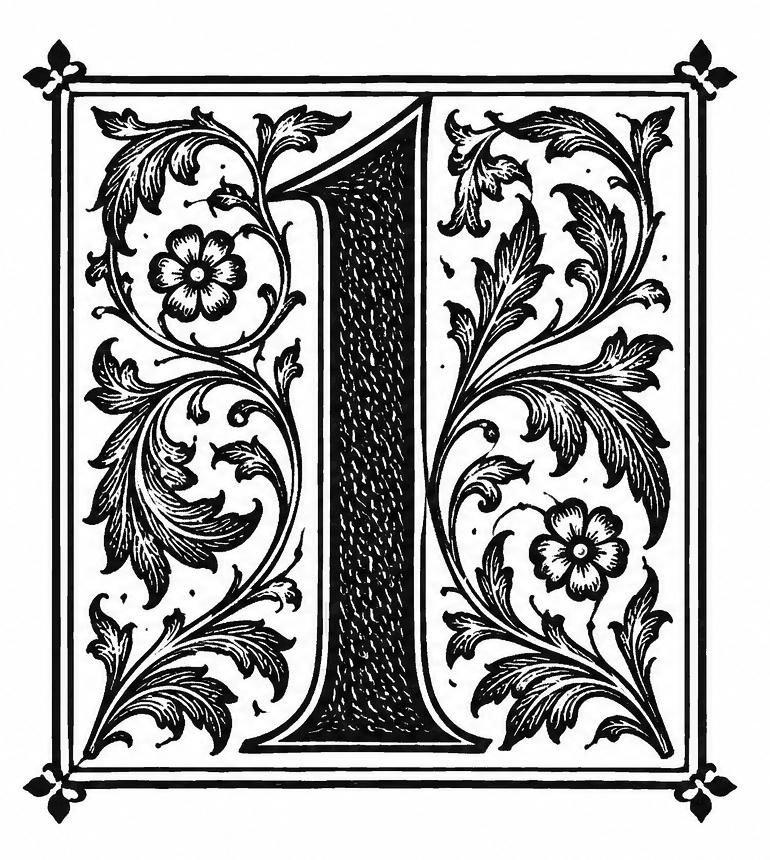
\includegraphics[width=2.5in]{drop_cap_1.png}
\caption{An ornamental numeral 1, the first appendix demonstration figure.}
\label{fig:app_numeral1}
\end{figure}

\begin{figure}
\centering
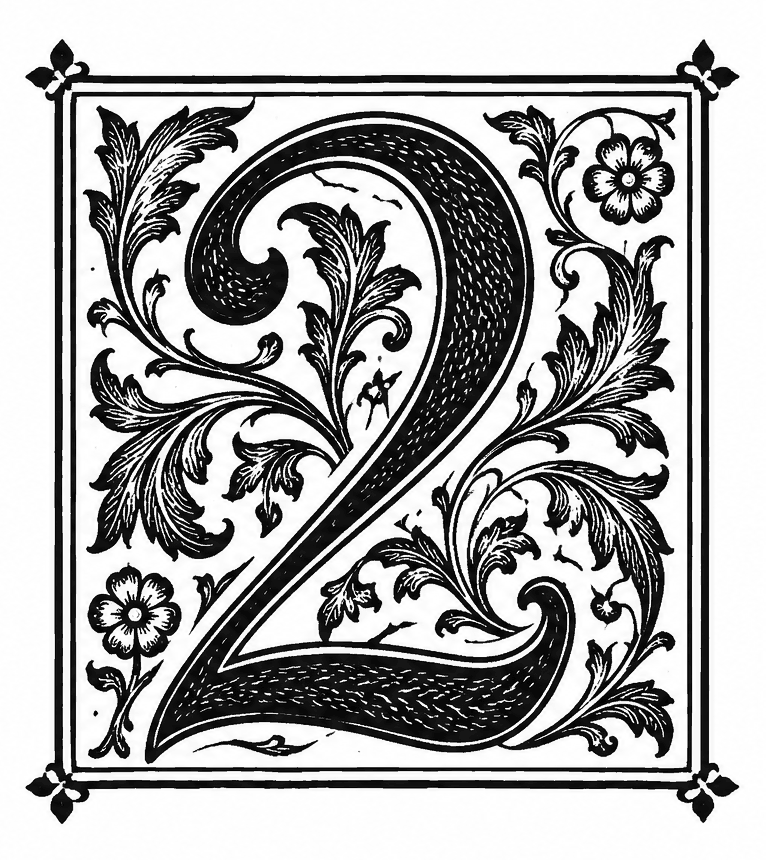
\includegraphics[width=2.5in]{drop_cap_2.png}
\caption{An ornamental numeral 2, the second appendix demonstration figure.}
\label{fig:app_numeral2}
\end{figure}

\section{Tables in an Appendix}

Here is an example of a table in an appendix showing how you might list websites you consulted. \cref{table:latexresources} lists free resources for learning \LaTeX\ and for answering questions as you write. The addresses are printed without the \texttt{https://} prefix, which keeps them short enough to fit the column, but each one still links to the full address:
\begin{verbatim}
\href{https://www.learnlatex.org}{\nolinkurl{www.learnlatex.org}}
\end{verbatim}
For an address printed in full, \verb+\url+ breaks long addresses at any character, thanks to the \texttt{xurl} package.

\begin{table}
\centering
\caption{Free Resources for Learning \LaTeX}
\label{table:latexresources}
\begin{tabularx}{\linewidth}{|>{\raggedright\arraybackslash}p{0.24\linewidth}|>{\raggedright\arraybackslash}p{0.36\linewidth}|>{\raggedright\arraybackslash}X|}
\hline
\textbf{Resource} & \textbf{Address} & \textbf{Good For} \\
\hline
Learn \LaTeX\ in 30 Minutes (Overleaf) & \href{https://www.overleaf.com/learn/latex/Learn_LaTeX_in_30_minutes}{\nolinkurl{www.overleaf.com/learn/latex/Learn_LaTeX_in_30_minutes}} & A first introduction, with examples you can edit online \\
\hline
learnlatex.org & \href{https://www.learnlatex.org}{\nolinkurl{www.learnlatex.org}} & Short interactive lessons covering the basics \\
\hline
Overleaf documentation & \href{https://www.overleaf.com/learn}{\nolinkurl{www.overleaf.com/learn}} & Task-based help on tables, figures, mathematics, and bibliographies \\
\hline
The Not So Short Introduction to \LaTeX & \href{https://ctan.org/pkg/lshort}{\nolinkurl{ctan.org/pkg/lshort}} & A complete free textbook \\
\hline
\LaTeX\ Wikibook & \href{https://en.wikibooks.org/wiki/LaTeX}{\nolinkurl{en.wikibooks.org/wiki/LaTeX}} & A searchable reference organized by topic \\
\hline
How Should We \LaTeX? (Roy Goodman) & \href{https://roygoodman.net/post/how-to-latex/}{\nolinkurl{roygoodman.net/post/how-to-latex}} & Style habits that manuals skip: meaningful macros, consistent notation, punctuating equations, and coauthoring \\
\hline
Short Math Guide for \LaTeX\ (AMS) & \href{https://ctan.org/pkg/short-math-guide}{\nolinkurl{ctan.org/pkg/short-math-guide}} & The commands of \texttt{amsmath} at a glance \\
\hline
Detexify & \href{https://detexify.kirelabs.org}{\nolinkurl{detexify.kirelabs.org}} & Finding the command for a symbol by drawing it \\
\hline
Comprehensive \LaTeX\ Symbol List & \href{https://ctan.org/pkg/comprehensive}{\nolinkurl{ctan.org/pkg/comprehensive}} & Every symbol available, with the package that provides it \\
\hline
TeX Stack Exchange & \href{https://tex.stackexchange.com}{\nolinkurl{tex.stackexchange.com}} & Answers to specific questions; search before asking \\
\hline
CTAN & \href{https://ctan.org}{\nolinkurl{ctan.org}} & Documentation for every package \\
\hline
\end{tabularx}
\end{table}

% \clearpage prints the floating Table A.1 first, so the tables stay in
% order; a longtable does not float and would otherwise come out first.
\clearpage
\section{Tables Longer Than One Page}

A table too long for one page is typed with the \texttt{longtable} environment instead of a \texttt{table} environment, as in \cref{table:longsample}. It does not float: it starts where it is typed and continues onto as many pages as it needs. Its title goes in the \verb+\endfirsthead+ part; the \verb+\endhead+ part, which starts with the class command \verb+\tablecontinued+, is repeated at the top of every later page, so each of them begins with ``\textbf{Table X.x (Continued)}'' and the column headings (GSO). The continued title is not listed again in the List of Tables.

\begin{longtable}{>{\centering\arraybackslash}p{0.15\linewidth}l>{\raggedright\arraybackslash}p{0.45\linewidth}}
\caption{Commands for Common Mathematical Symbols}
\label{table:longsample} \\
\toprule
\textbf{Symbol} & \textbf{Command} & \textbf{Meaning} \\
\midrule
\endfirsthead
\tablecontinued \\
\toprule
\textbf{Symbol} & \textbf{Command} & \textbf{Meaning} \\
\midrule
\endhead
\bottomrule
\endlastfoot
$\alpha$ & \verb+\alpha+ & Lowercase alpha \\
$\beta$ & \verb+\beta+ & Lowercase beta \\
$\gamma$ & \verb+\gamma+ & Lowercase gamma \\
$\delta$ & \verb+\delta+ & Lowercase delta \\
$\epsilon$ & \verb+\epsilon+ & Lowercase epsilon \\
$\zeta$ & \verb+\zeta+ & Lowercase zeta \\
$\eta$ & \verb+\eta+ & Lowercase eta \\
$\theta$ & \verb+\theta+ & Lowercase theta \\
$\iota$ & \verb+\iota+ & Lowercase iota \\
$\kappa$ & \verb+\kappa+ & Lowercase kappa \\
$\lambda$ & \verb+\lambda+ & Lowercase lambda \\
$\mu$ & \verb+\mu+ & Lowercase mu \\
$\nu$ & \verb+\nu+ & Lowercase nu \\
$\xi$ & \verb+\xi+ & Lowercase xi \\
$\pi$ & \verb+\pi+ & Lowercase pi \\
$\rho$ & \verb+\rho+ & Lowercase rho \\
$\sigma$ & \verb+\sigma+ & Lowercase sigma \\
$\tau$ & \verb+\tau+ & Lowercase tau \\
$\upsilon$ & \verb+\upsilon+ & Lowercase upsilon \\
$\phi$ & \verb+\phi+ & Lowercase phi \\
$\chi$ & \verb+\chi+ & Lowercase chi \\
$\psi$ & \verb+\psi+ & Lowercase psi \\
$\omega$ & \verb+\omega+ & Lowercase omega \\
$\varepsilon$ & \verb+\varepsilon+ & Variant of epsilon \\
$\vartheta$ & \verb+\vartheta+ & Variant of theta \\
$\varpi$ & \verb+\varpi+ & Variant of pi \\
$\varphi$ & \verb+\varphi+ & Variant of phi \\
$\Gamma$ & \verb+\Gamma+ & Uppercase gamma \\
$\Delta$ & \verb+\Delta+ & Uppercase delta \\
$\Theta$ & \verb+\Theta+ & Uppercase theta \\
$\Lambda$ & \verb+\Lambda+ & Uppercase lambda \\
$\Xi$ & \verb+\Xi+ & Uppercase xi \\
$\Pi$ & \verb+\Pi+ & Uppercase pi \\
$\Sigma$ & \verb+\Sigma+ & Uppercase sigma \\
$\Upsilon$ & \verb+\Upsilon+ & Uppercase upsilon \\
$\Phi$ & \verb+\Phi+ & Uppercase phi \\
$\Psi$ & \verb+\Psi+ & Uppercase psi \\
$\Omega$ & \verb+\Omega+ & Uppercase omega \\
$\nabla$ & \verb+\nabla+ & Gradient (nabla) \\
$\partial$ & \verb+\partial+ & Partial derivative \\
$\infty$ & \verb+\infty+ & Infinity \\
$\sum$ & \verb+\sum+ & Summation \\
$\prod$ & \verb+\prod+ & Product \\
$\int$ & \verb+\int+ & Integral \\
$\leq$ & \verb+\leq+ & Less than or equal to \\
$\geq$ & \verb+\geq+ & Greater than or equal to \\
$\neq$ & \verb+\neq+ & Not equal to \\
$\approx$ & \verb+\approx+ & Approximately equal to \\
$\in$ & \verb+\in+ & Element of \\
$\forall$ & \verb+\forall+ & For all \\
$\to$ & \verb+\to+ & Maps to, tends to \\
$\times$ & \verb+\times+ & Times, cross product \\
\end{longtable}

+ line if you have no appendix.
\item Write each chapter in its own file, \texttt{chapter1.tex}, \texttt{chapter2.tex}, and so on, and list them with \verb+\input+ in \texttt{main.tex}. While drafting, you can comment out finished chapters to compile faster. Start every new \texttt{.tex} file with the line \verb+% !TEX root = main.tex+ (\cref{subsec:editors}).
\item Put your sources in \texttt{references.bib} and your images in the \texttt{Graphics/} folder of the main folder. Replace the starter's placeholder entries in \texttt{references.bib}; this sample's \texttt{sample/references.bib} has a model of each common entry type.
\item Set the citation style for your discipline with the \texttt{style=} option on the \texttt{biblatex} line in \texttt{packages.tex}. \cref{tab:phd-styles} in \cref{sec:citestyles} lists the styles each program recommends, and \cref{ch:references} explains how to cite sources and build the bibliography.
\item Load any packages you need in \texttt{packages.tex}, before the \texttt{hyperref} line, and define your own notation and theorem environments in \texttt{macros.tex}.
\end{enumerate}
For a master's thesis, add the \texttt{thesis} option to the \verb+\documentclass+ line at the top of \texttt{main.tex}:
\begin{verbatim}
\documentclass[12pt,thesis]{njit_thesis}
\end{verbatim}
The title page then reads ``A Thesis'', the advisor is listed as ``Thesis Advisor'' on the approval page, and the copyright page is replaced by the blank page the GSO requires. In \texttt{biography.tex}, change \verb+\thisdegree+ to the full name of your master's degree, and if your degree is not a Master of Science, set the ``Degree:'' line of the Biographical Sketch with \verb+\degreelevel+. Two limits also change: a thesis abstract may be only one page long, where a dissertation abstract may be two, and a thesis committee needs at least three members, including the advisor, where a dissertation committee needs five. You should not need to edit the class file, \texttt{njit\_thesis.cls}.

To compile this sample, run \verb+latexmk -pdf main.tex+ in the \texttt{sample/} folder, or open \texttt{sample/main.tex} in TeXShop. It finds the class file, \texttt{packages.tex}, \texttt{macros.tex}, and the citation styles in the main folder through the paths \verb+../njit_thesis+ and \verb+../packages+. On Overleaf, read the sample as a PDF from the template's GitHub Releases page instead, because Overleaf expects the main file of a project in its top folder.

Keep your work safe from the first day. A lost laptop or an overwritten file a month before the deadline is a common disaster, and an easy one to prevent. Keep the folder under version control with Git (the free GitHub Desktop application is enough), or rely on Overleaf's history, and keep a second copy somewhere other than your own computer.

\section{Compiling the Dissertation}
\label{sec:compiling}
The subsections below describe several ways to compile. If compiling stops with an error that a \texttt{.sty} file was not found, a package the template needs is not installed; \cref{sec:missingpackages} explains how to find and install it.


\subsection{Recommended: \texttt{latexmk}}
The easiest and most reliable way to compile your dissertation locally is with \texttt{latexmk}:
\begin{verbatim}
latexmk -pdf main.tex
\end{verbatim}
\texttt{latexmk} monitors all file dependencies, automatically invokes \texttt{biber} for the bibliography and publications list, and runs \texttt{pdflatex} as many times as necessary to ensure all cross-references, Table of Contents entries, and list page numbers are completely up to date.

\subsection{Manual compilation steps}
If running commands manually in a terminal:
\begin{enumerate}
  \item \verb+pdflatex main.tex+ (generates auxiliary files and bibliography requests)
  \item \verb+biber main+ (processes \texttt{references.bib} and resolves citations)
  \item \verb+pdflatex main.tex+ (incorporates bibliography and generates cross-references)
  \item \verb+pdflatex main.tex+ (resolves final page numbers for TOC and lists)
\end{enumerate}

\subsection{Using Overleaf}
The template works on Overleaf without changes:
\begin{enumerate}
\item Download the template as a ZIP file and upload it to Overleaf with \emph{New Project}, then \emph{Upload Project}. You may delete the \texttt{sample/} folder from the project first; Overleaf compiles only the starter document.
\item In the project's \emph{Menu}, set the compiler to \textbf{pdfLaTeX} and the main document to \texttt{main.tex}.
\item Overleaf normally detects that the bibliography uses Biber. If the references show as ``??'', look for a bibliography setting in \emph{Menu} and choose \textbf{Biber}.
\end{enumerate}

\subsection{Using TeXShop, TeXstudio, or VS Code}
\label{subsec:editors}
Every \texttt{.tex} file in the template begins with the line
\begin{verbatim}
% !TEX root = main.tex
\end{verbatim}
This comment tells TeXShop on a Mac, and several other editors, to compile \texttt{main.tex} whichever file is open, so you can compile while editing a chapter. Keep it in every file, including new ones you create. In \texttt{main.tex}, the line \verb+% !TEX TS-program = pdflatexmk+ tells TeXShop to compile with \texttt{latexmk}, which runs Biber when needed. In other editors, choose pdf\LaTeX\ as the engine and Biber as the bibliography tool, or choose \texttt{latexmk}: in TeXstudio, under \emph{Options}, \emph{Configure TeXstudio}, \emph{Build}; in VS Code, with the LaTeX Workshop extension, whose default recipe uses \texttt{latexmk}.

\section{When Compiling Fails}
\label{sec:errors}
When \LaTeX\ meets something it cannot handle, it stops and prints an error that begins with an exclamation mark, followed by the line where it noticed the problem:
\begin{verbatim}
! Undefined control sequence.
l.42 The value of \alpah
\end{verbatim}
Read the first error only; later errors are often caused by the first one. The number after \texttt{l.} is the line in the file being read, and the error is usually on that line or just before it. If the compiler stops with a \texttt{?} prompt, type \texttt{X} and press Enter to quit, fix the line, and compile again. The most common errors are:
\begin{itemize}
\item \textbf{Undefined control sequence}: A command is misspelled, as in \verb+\alpah+ above, or comes from a package that is not loaded.
\item \textbf{Missing \$ inserted}: A math command such as \verb+^+, \verb+_+, or \verb+\alpha+ is used outside math mode, or a \verb+$+ is missing.
\item \textbf{Missing \} inserted, or Runaway argument}: A brace \verb+{+ is not closed. Check the lines just before the one reported.
\item \textbf{File not found}: A package or image is missing, or its name is misspelled. For packages, see \cref{sec:missingpackages}; for images, check the name and the \texttt{Graphics/} folder.
\item \textbf{Citation or reference undefined (a warning, shown as ``??'')}: Compile again; if it persists, the key in \verb+\cite+ or \verb+\ref+ does not match any \verb+\label+ or \texttt{.bib} entry.
\end{itemize}
If the PDF does not change or the errors make no sense, delete the auxiliary files (\cref{app:filetree} lists them) and compile again. If you are stuck, search for the exact error message; TeX Stack Exchange (\url{https://tex.stackexchange.com}) has answers to almost all of them.

% !TEX root = main.tex
% Chapter 2: the parts of a dissertation, in the GSO's order, and the
% formatting rules the template applies for you.
%
% Each chapter lives in its own file, included from main.tex with \input.
% Start the file with \chapter{Title}; type the title in normal
% capitalization (the class sets it in capitals). Headings below it:
%   \section       level 2, Title Case
%   \subsection    level 3, sentence case
%   \subsubsection level 4, sentence case, run-in (the class adds the period)
%   \paragraph     level 5, sentence case, italic (the class adds the period)
% Every heading needs a title; an empty one stops the build with an error.

\chapter{What the GSO Requires}
\label{ch:requirements}

The Graduate Studies Office (GSO) checks every dissertation against its formatting rules before accepting it. This chapter lists the parts a dissertation must contain, in the required order, and shows which rules the template applies for you and which are up to you.

\section{The Parts of a Dissertation, in Order}

An NJIT dissertation consists of three primary divisions: the preliminary front matter, the main body (the chapters), and the back matter (the References and any appendices). These components appear in the following strict order:

\begin{itemize}
\emergencystretch=2em
\item \textbf{Abstract}: A concise summary of the research questions, methodology, and conclusions. By NJIT guidelines, this page is unnumbered and precedes the title page. Written in \texttt{abstract.tex}.

\item \textbf{Title Page}: The formal title page declaring degree, department, joint institution (if applicable), and graduation month and year. This page is considered Roman numeral~i, but no number is displayed on the page. Built from the information in \texttt{biography.tex}.

\item \textbf{Copyright Page}: Declares the copyright holder and year. Unnumbered. Required only for doctoral dissertations; a master's thesis has a blank page in its place (GSO), which the \texttt{thesis} class option produces. Built automatically.

\item \textbf{Approval Page}: Contains the signature lines for the dissertation advisor (and co-advisor, if any) and committee members with their official academic titles as listed in the graduate catalog. Unnumbered. Configured in \texttt{approval.tex}.

\item \textbf{Biographical Sketch}: Displays academic background, degrees earned (in reverse chronological order), major field of study, and a listing of presentations and publications. Roman page numbering begins visibly here (typically on page~iv). Configured in \texttt{biography.tex}. The publication list is generated automatically via \BibTeX\ / \texttt{biblatex} using the keyword \texttt{me}.

\item \textbf{Dedication} (optional): A brief personal dedication. Centered and formatted with single spacing. Written in \texttt{dedication.tex}.

\item \textbf{Acknowledgments}: Formal recognition of academic guidance, committee assistance, grant funding and financial support, technical and administrative assistance, and personal gratitude. Written in \texttt{acknowledgment.tex}. The command \verb+\initthesis+ in \texttt{main.tex} prints all of the pages from the Abstract to this one, in this order. (Behind the scenes it calls \verb+\makeabstract+, \verb+\maketitle+, and so on, one command per page.)

\item \textbf{Table of Contents}: Lists the chapters, their sections (X.x) and subsections (X.x.x), the References, and the appendices, with dot leaders connecting titles to page numbers. It starts at Chapter~1: the front matter and the lists that follow the Table of Contents are not included (GSO). Generated automatically by \verb+\tableofcontents+.

\item \textbf{List of Tables}: Generated automatically by \verb+\listoftables+. If your dissertation contains no tables, comment out this command in \texttt{main.tex}.

\item \textbf{List of Figures}: Generated automatically by \verb+\listoffigures+. If your dissertation contains no figures, comment out this command in \texttt{main.tex}.

\item \textbf{List of Algorithms} (optional): Generated automatically by \verb+\listofalgorithms+ from the \texttt{algorithm} environments (\cref{sec:source_code}). The starter document has this command commented out in \texttt{main.tex}; uncomment it if your dissertation contains algorithms.

\item \textbf{List of Symbols} (optional): Defines mathematical symbols and physical constants used throughout the text. Organize the list in one of three ways: by category or function, alphabetically by name, or by frequency of use. An alphabetical list follows the order of the characters themselves, so a symbol such as $*$ comes after $\&$. Configured in \texttt{listofsymbols.tex} and printed by \verb+\makelistofsymbols+ in \texttt{main.tex}. The starter document leaves it out; \cref{sec:setup} explains how to add it.

\item \textbf{Glossary of Terms} (optional): An alphabetical list of definitions. Configured in \texttt{listofdefinitions.tex} and printed by \verb+\makeglossaryofterms+ in \texttt{main.tex}. The starter document leaves it out as well.


\item \textbf{Main Body}: The dissertation chapters, beginning with Arabic page number~1 at \verb+\startbody+. Each chapter is housed in its own file (e.g., \texttt{chapter1.tex}, \texttt{chapter2.tex}). Page numbers are centered at the bottom of every page in bold (GSO).

\item \textbf{References}: The bibliography, styled consistently and sorted according to the field's standard conventions. It comes right after the last chapter, before all of the appendices (GSO). Generated from \texttt{references.bib} via \texttt{biblatex} and \texttt{biber}.

\item \textbf{Appendices}: Supplementary mathematical proofs, data tables, or algorithm listings. NJIT enforces a strict rule: if there is only a \textbf{single appendix}, it must be labeled \textbf{APPENDIX} (without a letter like "A"). If there are \textbf{multiple appendices}, they must be numbered \textbf{APPENDIX A}, \textbf{APPENDIX B}, etc. This template fully automates both cases; \cref{app:appendixA} explains how, and what material belongs in an appendix. If you upload supplementary files to ProQuest, such as videos, data sets, or software archives, list them in the last appendix (GSO). Short sections of text, such as computer code, can be included there as well. \texttt{supplementary.tex} shows how to list the files, and produces \cref{app:supplementary} of this sample.
\end{itemize}

\section{What the Template Does for You}
\label{sec:template-does}

The class file applies most of the GSO's formatting rules automatically. \cref{table:gso_rules} lists the main rules and shows which ones the template takes care of and which are up to you.

% !TEX root = main.tex
% Sample table, kept in its own file and included from chapter2.tex with
% % !TEX root = main.tex
% Sample table, kept in its own file and included from chapter2.tex with
% \input{table}. Separate files are optional but handy for large tables or
% tables generated by a script.
%
% GSO rules (the class handles the layout):
% - The title (\caption) goes ABOVE the table, in title case, with no final
%   period. It appears word for word in the List of Tables.
% - Tables are numbered by chapter (Table 1.1).
% - Table text is single-spaced. Do not split a table across pages if it
%   fits on a single page; a longer table is a longtable with \tablecontinued
%   in its \endhead, which prints "Table X.x (Continued)" on each page after
%   the first (see Table A.2 in appendix-demo.tex).
% - The source of a borrowed table goes below the table: \floatsource{...}
%   after the tabular.
% Refer to every table in the text with \cref{label}.

\begin{table}
\centering
\caption{GSO Formatting Rules and How the Template Handles Them}
\label{table:gso_rules}

\begin{tabularx}{\linewidth}{|>{\raggedright\arraybackslash}p{0.16\linewidth}|>{\raggedright\arraybackslash}X|>{\raggedright\arraybackslash}X|}
\hline
\textbf{Element} & \textbf{GSO Rule} & \textbf{In This Template} \\
\hline
Margins & 1.5 in on the left; 1 in at the top, bottom, and right & Automatic \\
\hline
Font & Times New Roman or Arial, 12 pt, including headings & Automatic (Times, through \texttt{newtx}) \\
\hline
Spacing & Text double-spaced, paragraphs indented 0.5 in; one blank line above a level 2 heading and none above levels 3 to 5; headings, captions, tables, lists, code, algorithms, and references single-spaced & Automatic \\
\hline
Page numbers & Bold, centered at the bottom; title page counts as i; first number shown is iv, on the Biographical Sketch; Arabic numbering starts at Chapter 1 & Automatic \\
\hline
Front matter & Fixed order, from the abstract to the lists; copyright page for dissertations only & Automatic; use the \texttt{thesis} class option for a master's thesis \\
\hline
Dates & Graduation month and year, not the defense date & Set \texttt{\textbackslash graduationdate} in \texttt{biography.tex} \\
\hline
Names and titles & Faculty titles exactly as in the Graduate Catalog & Check them yourself in \texttt{approval.tex} \\
\hline
Headings & Every heading numbered and titled; level 2 in title case, levels 3 to 5 in sentence case & Layout automatic; you type the capitalization \\
\hline
Table of Contents & Starts at Chapter 1; chapter titles in capitals; dot leaders; ``(Continued)'' on later pages & Automatic \\
\hline
Captions & Table titles above, figure captions below; numbered by chapter; table titles in title case with no final period; the source of a borrowed figure, table, or algorithm on a single-spaced 10 pt line below it & Layout automatic; you write the titles and the \texttt{\textbackslash floatsource} line \\
\hline
Appendices & One appendix is ``APPENDIX''; several are ``APPENDIX A'', ``APPENDIX B'', and so on; each opens with introductory text & Labels automatic; you write the introduction \\
\hline
References & The citation style used in your discipline & Set \texttt{style=} on the \texttt{biblatex} line in \texttt{packages.tex} \\
\hline
\end{tabularx}
\end{table}
. Separate files are optional but handy for large tables or
% tables generated by a script.
%
% GSO rules (the class handles the layout):
% - The title (\caption) goes ABOVE the table, in title case, with no final
%   period. It appears word for word in the List of Tables.
% - Tables are numbered by chapter (Table 1.1).
% - Table text is single-spaced. Do not split a table across pages if it
%   fits on a single page; a longer table is a longtable with \tablecontinued
%   in its \endhead, which prints "Table X.x (Continued)" on each page after
%   the first (see Table A.2 in appendix-demo.tex).
% - The source of a borrowed table goes below the table: \floatsource{...}
%   after the tabular.
% Refer to every table in the text with \cref{label}.

\begin{table}
\centering
\caption{GSO Formatting Rules and How the Template Handles Them}
\label{table:gso_rules}

\begin{tabularx}{\linewidth}{|>{\raggedright\arraybackslash}p{0.16\linewidth}|>{\raggedright\arraybackslash}X|>{\raggedright\arraybackslash}X|}
\hline
\textbf{Element} & \textbf{GSO Rule} & \textbf{In This Template} \\
\hline
Margins & 1.5 in on the left; 1 in at the top, bottom, and right & Automatic \\
\hline
Font & Times New Roman or Arial, 12 pt, including headings & Automatic (Times, through \texttt{newtx}) \\
\hline
Spacing & Text double-spaced, paragraphs indented 0.5 in; one blank line above a level 2 heading and none above levels 3 to 5; headings, captions, tables, lists, code, algorithms, and references single-spaced & Automatic \\
\hline
Page numbers & Bold, centered at the bottom; title page counts as i; first number shown is iv, on the Biographical Sketch; Arabic numbering starts at Chapter 1 & Automatic \\
\hline
Front matter & Fixed order, from the abstract to the lists; copyright page for dissertations only & Automatic; use the \texttt{thesis} class option for a master's thesis \\
\hline
Dates & Graduation month and year, not the defense date & Set \texttt{\textbackslash graduationdate} in \texttt{biography.tex} \\
\hline
Names and titles & Faculty titles exactly as in the Graduate Catalog & Check them yourself in \texttt{approval.tex} \\
\hline
Headings & Every heading numbered and titled; level 2 in title case, levels 3 to 5 in sentence case & Layout automatic; you type the capitalization \\
\hline
Table of Contents & Starts at Chapter 1; chapter titles in capitals; dot leaders; ``(Continued)'' on later pages & Automatic \\
\hline
Captions & Table titles above, figure captions below; numbered by chapter; table titles in title case with no final period; the source of a borrowed figure, table, or algorithm on a single-spaced 10 pt line below it & Layout automatic; you write the titles and the \texttt{\textbackslash floatsource} line \\
\hline
Appendices & One appendix is ``APPENDIX''; several are ``APPENDIX A'', ``APPENDIX B'', and so on; each opens with introductory text & Labels automatic; you write the introduction \\
\hline
References & The citation style used in your discipline & Set \texttt{style=} on the \texttt{biblatex} line in \texttt{packages.tex} \\
\hline
\end{tabularx}
\end{table}


% !TEX root = main.tex
% Chapter 3: writing the text: headings, mathematics and units, code and
% pseudocode, cross-references, and common typing mistakes.
%
% Each chapter lives in its own file, included from main.tex with \input.
% Start the file with \chapter{Title}; type the title in normal
% capitalization (the class sets it in capitals). Headings below it:
%   \section       level 2, Title Case
%   \subsection    level 3, sentence case
%   \subsubsection level 4, sentence case, run-in (the class adds the period)
%   \paragraph     level 5, sentence case, italic (the class adds the period)
% Every heading needs a title; an empty one stops the build with an error.

\chapter{Writing the Text}
\label{ch:writing}

This chapter covers the parts of the text you type yourself: headings, mathematics, code, and cross-references, and the typing conventions that \LaTeX\ expects.

\section{Section Headings and Hierarchy}
\label{sec:headings}

The GSO recognizes five levels of headings. The class file formats each level for you; what you control is the \emph{capitalization} of the text you type, because \LaTeX\ cannot reliably convert titles to title case.

\begin{itemize}
\item \textbf{Level 1, \texttt{\textbackslash chapter}}: Bold, all capitals, centered. Type the title normally; the class capitalizes it.
\item \textbf{Level 2, \texttt{\textbackslash section} (X.x)}: Bold, centered, in \textbf{title case}: Capitalize Every Word Except Articles, Prepositions, and Conjunctions.
\item \textbf{Level 3, \texttt{\textbackslash subsection} (X.x.x)}: Bold, flush left, in \textbf{sentence case}: only the first word and proper names are capitalized.
\item \textbf{Level 4, \texttt{\textbackslash subsubsection} (X.x.x.x)}: Bold, sentence case, ending with a period, with the text continuing on the same line after a tab. Not listed in the Table of Contents.
\item \textbf{Level 5, \texttt{\textbackslash paragraph} (X.x.x.x.x)}: Italic, not bold, sentence case, ending with a period, with the text beginning on the next line. Not listed in the Table of Contents.
\end{itemize}

The class adds the period after level~4 and~5 titles, so do not type one. Every heading must have a title: an empty title, such as \verb+\section{}+, stops the build with an error that names the line. Every heading below the chapter level must also be numbered, because the style guide does not allow unnumbered sections. If you use a starred command such as \verb+\section*+, the class prints its title in red and writes a warning to the log; remove the \verb+*+ to fix it. Use the same levels consistently in every chapter, and do not skip a level (a \verb+\subsubsection+ belongs inside a \verb+\subsection+). If you find yourself needing levels~4 and~5 often, consider whether the chapter should be split. Give every heading a different title: no two sections or subsections anywhere in the dissertation may have the same title (GSO). The rest of this section demonstrates levels 3 to 5.

\subsection{Third level subsection headings}
\label{subsec:subsections}
Subsection headings (level 3, X.x.x) are flush left, bold, and in sentence case. Notice that subsections are numbered within the chapter, such as \cref{subsec:subsections}.

\subsubsection{Fourth level subsection headings}
\label{subsubsec:subsubsections}
Subsubsections (level 4, X.x.x.x) are bold and in sentence case, and the text continues on the same line after a tab. The class adds the period after the title, so do not type one. They do not appear in the Table of Contents.

\paragraph{Fifth level subsection headings}
The \verb+\paragraph+ command gives level 5 (X.x.x.x.x): numbered, italic, in sentence case, followed by a period, with the text starting on the next line. Like level 4, it does not appear in the Table of Contents.

\section{Mathematics, Symbols, and Units}
\label{sec:math}

The template preconfigures the standard American Mathematical Society (\AmS) packages \texttt{amsmath} and \texttt{amsthm}, together with \texttt{mathtools}; the AMS symbols come with the \texttt{newtxmath} font package. Students in applied mathematics and physics may also want two more packages, which replace the older \texttt{physics} package, unmaintained since 2012. The \texttt{derivative} package handles derivatives and differentials: \verb+\odv{y}{x}+ gives $\frac{\mathrm{d}y}{\mathrm{d}x}$, \verb+\pdv{f}{x,y}+ a mixed partial derivative, and \verb+\odif{x}+ gives the upright $\mathrm{d}x$ of an integral with the right spacing. The \texttt{physics2} package provides automatically sized delimiters, bra--ket notation, and matrices, in modules you enable after loading it: \verb+\usephysicsmodule{ab,ab.braket,diagmat,xmat}+. Neither package is loaded by the template, so add them in \texttt{packages.tex}; the guide \emph{How Should We \LaTeX?} in \cref{table:latexresources} shows both in use. Here are some examples.

\begin{definition}[Sobolev Space $H^1(\RR)$]
\label{def:sobolev}
The Sobolev space $H^1(\RR)$ is defined as the Hilbert space of all square-integrable functions whose weak derivative is also square-integrable:
\begin{equation}
\label{eq:sobolev}
H^1(\RR) = \left\{ u \in L^2(\RR) \;\middle|\; \frac{du}{dx} \in L^2(\RR) \right\},
\end{equation}
equipped with the inner product
\begin{equation}
\label{eq:innerprod}
\langle u, v \rangle_{H^1} = \int_{-\infty}^{\infty} \left( u(x)v(x) + \frac{du}{dx}\frac{dv}{dx} \right) \, dx.
\end{equation}
\end{definition}

\begin{theorem}[Energy--Mass Equivalence]
\label{thm:einstein}
For a particle of invariant rest mass $m$ at rest in an inertial reference frame, its total relativistic energy $E$ satisfies
\begin{equation}
\label{eq:einstein}
E = m c^2,
\end{equation}
where $c \approx \qty{3e8}{\metre\per\second}$ is the speed of light in vacuum.
\end{theorem}

\begin{proof}
In relativistic mechanics, the four-momentum $P^\mu = (E/c, \bm{p})$ satisfies the dispersion relation $P^\mu P_\mu = (E/c)^2 - |\bm{p}|^2 = m^2 c^2$. Setting the spatial momentum $\bm{p} = \bm{0}$ yields $(E/c)^2 = m^2 c^2$, whence $E = mc^2$.
\end{proof}

You can cross-reference equations easily: for example, see \cref{eq:einstein} or \cref{def:sobolev}. Both were typed with \verb+\cref+, which adds the name (and, for equations, the parentheses) automatically; \cref{sec:crossrefs} explains cross-references in more detail. The bold vector $\bm{p}$ is typed \verb+\bm{p}+, from the \texttt{bm} package.

\textbf{Equation numbering.} Equations are numbered by chapter, not by section, as in \cref{eq:einstein} (GSO). The class does this automatically. Number only the equations you refer to later; use \verb+equation*+ or \verb+\nonumber+ for the rest.

Displayed equations are part of the sentence that introduces them and take punctuation accordingly: a comma or period at the end of the display, inside the math. Never refer to an equation by typing its number; always use \verb+\label+ and \verb+\eqref+, so the numbers stay correct when you move material between chapters. Leave room around displays, and do not use \verb+\vspace+ to squeeze equations onto a page.

\textbf{Theorems.} Theorems, lemmas, definitions, and the like share one counter and are numbered by chapter. Add new environments in \texttt{macros.tex}, not in the chapter files, so they are numbered consistently.


\textbf{Symbols.} The template supports inline symbols and notation. Defined symbols (such as $E$ for energy, $m$ for mass, and $c$ for speed of light) can be summarized in the dedicated List of Symbols generated before Chapter~1 via \texttt{listofsymbols.tex}. Brand names can carry a trademark sign with the \verb+\trademark+ command defined in \texttt{macros.tex}, as in MATLAB\trademark.

\textbf{Numbers and units.} Type quantities with the \texttt{siunitx} package rather than by hand, so that numbers, units, and the space between them are set the same way everywhere. For example:
\begin{itemize}
\item \verb+\qty{3e8}{\metre\per\second}+ gives \qty{3e8}{\metre\per\second};
\item \verb+\num{0.000125}+ gives \num{0.000125};
\item \verb+\unit{\kilo\gram\per\cubic\metre}+ gives \unit{\kilo\gram\per\cubic\metre};
\item \verb+\qtyrange{10}{20}{\celsius}+ gives \qtyrange{10}{20}{\celsius}.
\end{itemize}
The same commands work in text and in math. In a table, the column type \texttt{S} lines numbers up on their decimal points.

\section{Source Code and Pseudocode}
\label{sec:source_code}

If your dissertation has a computational component, you may want to include source code. The listing below uses the \texttt{lstlisting} environment from the \texttt{listings} package, loaded in \texttt{packages.tex}. The option \texttt{language=Matlab} chooses which words are highlighted; change it to match your code, for example \texttt{language=Python} or \texttt{language=C}.

\begin{lstlisting}[language=Matlab]
%%%%% BEGIN MATLAB CODE LISTING %%%%%
x=linspace(0,2*pi);  % set up the x-values
y=sin(x);            % set up the y-values
plot(x,y);           % plot the result
if 0>1
  fprintf('Zero is greater than one\n')
end
%%%%%  END MATLAB CODE LISTING  %%%%%
\end{lstlisting}

Source code and pseudocode are single-spaced (GSO); the class does this for you. Syntax highlighting in color is allowed.

\textbf{Pseudocode.} To describe an algorithm without tying it to one programming language, write it as pseudocode with the \texttt{algorithmic} environment from the \texttt{algpseudocode} package, and put it in an \texttt{algorithm} environment, as in \cref{alg:bisection}. The \texttt{algorithm} environment works like a table: give it a \verb+\caption+, typed in title case, and a \verb+\label+. The class numbers it by chapter, sets its title above it between two rules, and lists it in the List of Algorithms. Do not put an algorithm in a \texttt{figure} environment; the GSO does not count it as a figure. Like a figure, an algorithm must fit on one page. An algorithm taken or adapted from another source, such as a textbook, needs a credit line like the one for a figure you did not create (\cref{sec:figurepermission}): type \verb+\floatsource{...}+ after the \texttt{algorithmic} environment, as in \cref{alg:bisection}.

\begin{algorithm}
\caption{Bisection Method for a Root of a Continuous Function}
\label{alg:bisection}
\begin{algorithmic}[1]
\Require a continuous function $f$, an interval $[a,b]$ with $f(a)f(b)<0$, and a tolerance $\varepsilon>0$
\Ensure a point within $\varepsilon$ of a root of $f$
\While{$b-a > 2\varepsilon$}
  \State $m \gets (a+b)/2$
  \If{$f(a)f(m) \le 0$}
    \State $b \gets m$
  \Else
    \State $a \gets m$
  \EndIf
\EndWhile
\State \Return $(a+b)/2$
\end{algorithmic}
\floatsource{Adapted from \cite{BurdenFaires2011}, Algorithm~2.1.}
\end{algorithm}

\section{Cross-References and Links}
\label{sec:crossrefs}

Never type the number of a chapter, section, equation, figure, table, or page. Put a \verb+\label+ on the item and refer to it by that label, so the numbers stay correct when you add or move material.
\begin{itemize}
\item Place \verb+\label+ right after \verb+\caption+ in a figure or table, right after the heading command for a chapter or section, and inside the environment for an equation or theorem. A \verb+\label+ placed before \verb+\caption+ points to the section instead of the figure.
\item Start each label with a prefix that says what it is, such as \texttt{fig:}, \texttt{tab:}, \texttt{eq:}, \texttt{sec:}, or \texttt{ch:}. Labels never appear in the PDF, so keep them short and without spaces.
\item \verb+\cref+, which this sample uses, prints the name and the number together. Typing \verb+\cref{eq:sobolev,eq:innerprod}+ gives ``\cref{eq:sobolev,eq:innerprod}'', and typing \verb+\cref{fig:eberhardt}+ gives ``\cref{fig:eberhardt}''. It comes from the \texttt{cleveref} package.
\item With \verb+\ref+ you type the name yourself. Put a tie (\verb+~+) between the name and the reference, as in \verb+Figure~\ref{fig:eberhardt}+, so that a line break never separates them. For equations, use \verb+\eqref+, which adds the parentheses. For example, ``Equation~\eqref{eq:einstein}'' is typed as \verb+Equation~\eqref{eq:einstein}+.
\item \verb+\pageref+ gives the page an item is on, as in ``page~\pageref{fig:eberhardt}''.
\item Until every reference is resolved, \LaTeX\ prints ``??'' in place of the number. Compile until the log no longer reports undefined references.
\end{itemize}
Choose either \verb+\cref+ or \verb+\ref+ and use it throughout the document. This sample uses \verb+\cref+ everywhere except in the examples above.

The \texttt{hyperref} package, loaded at the end of \texttt{packages.tex}, turns every cross-reference, citation, and Table of Contents entry into a link in the PDF, and adds bookmarks for the chapters and sections. The links are not colored, so the printed pages look the same. For a web address, use \verb+\url{https://ctan.org}+, which breaks long addresses at the end of a line, or \verb+\href{https://ctan.org}{CTAN}+ to make a word into a link.

\section{Common Typing Mistakes}
\label{sec:typing}

\LaTeX\ handles most typography for you, but a few things depend on what you type.\footnote{A footnote is typed with \texttt{\textbackslash footnote\{...\}} right where its mark should appear, with no space before it. The class sets footnotes single-spaced at the bottom of the page and numbers them through each chapter.}
\begin{itemize}
\item \textbf{Quotation marks}: Type \verb+``this''+, with two grave accents and two apostrophes. In this template you can also type plain double quotes, \verb+"this"+, because the \texttt{csquotes} package converts them.
\item \textbf{Dashes}: A hyphen (\verb+-+) joins words, as in ``well-posed''. An en dash (\verb+--+) marks a range, as in pages 19--48. An em dash (\verb+---+) sets off a phrase. A minus sign belongs in math mode: type \verb+$-1$+, not \verb+-1+.
\item \textbf{Spaces after periods}: \LaTeX\ puts extra space after a period it takes to end a sentence. After an abbreviation, type a backslash and a space, or a tie: \verb+e.g.\ this+, \verb+Dr.~Smith+. When a sentence ends with a capital letter, type \verb+\@+ before the period: \verb+measured by NASA\@.+
\item \textbf{Ellipsis}: Type \verb+\ldots+, not three periods. In math, use \verb+\dots+ or \verb+\cdots+.
\item \textbf{Math in the text}: Put every variable in math mode, even a single letter: \verb+$x$+, not \verb+x+. Use \verb+\text{...}+ for words inside math, and \verb+\sin+, \verb+\log+, or \verb+\max+ for function names, so they are set upright.
\item \textbf{Spacing and layout}: Leave a blank line between paragraphs. Do not end lines with \verb+\\+, and do not adjust the layout with \verb+\vspace+ or \verb+\newpage+; the class sets all the spacing the GSO requires.
\item \textbf{Special characters}: The characters \verb+# $ % & _ { } ~ ^ \+ have special meanings. To print them, type \verb+\#+, \verb+\$+, \verb+\%+, \verb+\&+, \verb+\_+, \verb+\{+, \verb+\}+, \verb+\textasciitilde+, \verb+\textasciicircum+, and \verb+\textbackslash+.
\end{itemize}

% !TEX root = main.tex
% Chapter 4: figures, exporting plots, reusing figures, and tables.
%
% Each chapter lives in its own file, included from main.tex with \input.
% Start the file with \chapter{Title}; type the title in normal
% capitalization (the class sets it in capitals). Headings below it:
%   \section       level 2, Title Case
%   \subsection    level 3, sentence case
%   \subsubsection level 4, sentence case, run-in (the class adds the period)
%   \paragraph     level 5, sentence case, italic (the class adds the period)
% Every heading needs a title; an empty one stops the build with an error.

\chapter{Figures and Tables}
\label{ch:figtables}

This chapter explains how to place figures and tables, how to export plots so they look right on the page, and when you need permission to reuse a figure.

\section{Figures and Subfigures}
\label{sec:figures}

Every figure must be placed in a \texttt{figure} environment with a \verb+\caption+ and a \verb+\label+. The rules, all handled by the class except where noted:
\begin{itemize}
\item Figures are numbered by chapter: \cref{fig:eberhardt} is the first figure in \cref{ch:figtables} (GSO).
\item The caption goes \textbf{below} the figure, single-spaced and left-justified. The label is bold and followed by two spaces, with no colon (``\textbf{\cref{fig:eberhardt}}'').
\item The caption text appears word for word in the List of Figures, so do not use the short-caption form \verb+\caption[short]{long}+.
\item A figure and its caption must be on the same page, and a figure may not continue onto a second page (GSO). (Not handled by the class.)
\item A page that holds only figures or tables starts them at the top of the page.
\item Refer to every figure in the text, before or near where it appears, using \verb+\cref+ or \verb+\ref+ (\cref{sec:crossrefs}). (Not handled by the class.)
\item A caption should say what the figure shows and give anything the reader needs to interpret it. Keep advice and discussion in the text, because the whole caption is repeated in the List of Figures.
\item The source of a figure you did not create does \textbf{not} go in the caption, so it does not appear in the List of Figures. Put it on its own line below the caption, single-spaced, in 10~pt type, with \verb+\floatsource{...}+ after the \verb+\caption+, as in \cref{fig:eberhardt} (GSO).
\item Run spell-check on the text \emph{inside} your figures, such as axis labels and legends; the GSO checks it. (Not handled by the class.)
\end{itemize}
Make sure figures are legible at their printed size: axis labels and legends should be no smaller than about 8--10\,pt after scaling. \Cref{sec:exportplots} explains how to export plots at the right size from MATLAB, Mathematica, and Python. Let \LaTeX\ place floats. The class gives every figure, table, and algorithm the placement option \verb+[htbp]+ by default, which lets \LaTeX\ put it here, at the top or bottom of a page, or on a page of floats, so the sample never types an option after \verb+\begin{figure}+. You should usually not change it: forcing a position, for example with \verb+[h]+ or \verb+[H]+, usually produces large gaps.

\begin{figure}
\centering
% Place a photograph at Graphics/EberhardtHall.jpg. Until then a framed
% placeholder of the same size is printed, so the document still compiles.
\IfFileExists{Graphics/EberhardtHall.jpg}%
  {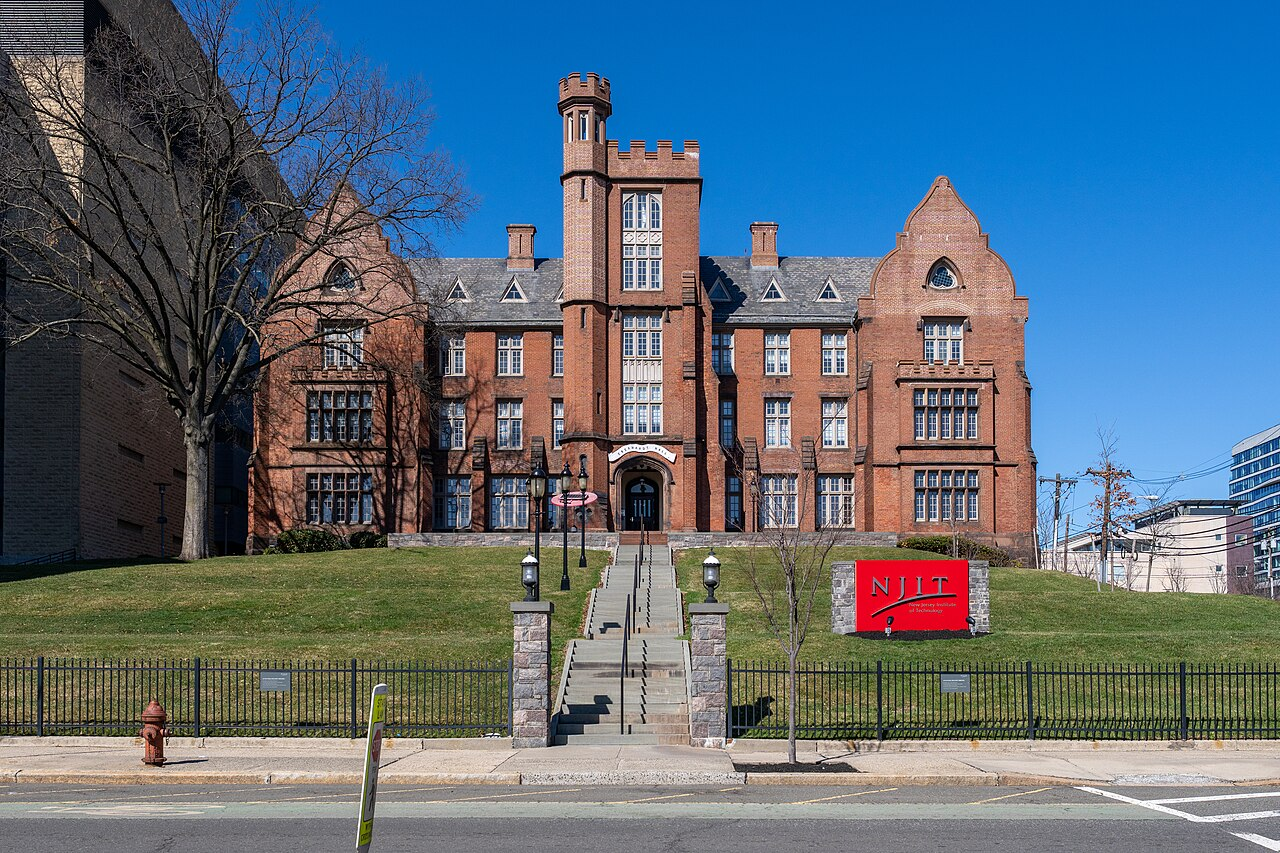
\includegraphics[width=4in]{EberhardtHall.jpg}}%
  {\fbox{\parbox[c][2.6in][c]{3.9in}{\centering Photograph of Eberhardt Hall\\(add \texttt{Graphics/EberhardtHall.jpg})}}}
\caption{Eberhardt Hall, the oldest building on the NJIT campus, built in 1857 as the Newark Orphan Asylum and restored in 2005 as the university's alumni center.}
\label{fig:eberhardt}
\floatsource{\cite{EberhardtWiki}. Photograph by Ajay Suresh, licensed under CC~BY~4.0.}
\end{figure}

A plot is read at its printed size, often on paper and sometimes in black and white. \Cref{fig:badplot,fig:goodplot} plot the same two curves. \Cref{fig:badplot} has faults that are common in dissertations, and the red cross marks it as an example not to follow:
\begin{itemize}
\item The curves are hairlines, which almost vanish in print. Draw curves at least 1~pt wide.
\item The legend text is about 4~pt, and the legend sits on top of the data. Legend text, like all text in a figure, should be about 8 to 10~pt, and the legend should hide nothing.
\item The labels are in Helvetica and the tick numbers in Computer Modern, and neither matches the Times text around the figure.
\item The two curves differ only in color, red and green, which look alike in black-and-white print and to readers with the most common kind of color blindness. Use different line styles as well, such as solid and dashed.
\item The green is pure green, RGB $[0\ 1\ 0]$, the default \texttt{'g'} in MATLAB. It is so light that it nearly disappears against a white background. Choose dark colors, such as MATLAB's default color order, rather than pure red, green, or blue.
\item The axis labels, t and x1, are variable names from the code, with no units, and the tick numbers carry three meaningless decimal places.
\item The heavy grid competes with the data.
\end{itemize}
\Cref{fig:goodplot} fixes each fault. It was also drawn at its printed size, 4 inches wide, and included without a \texttt{width} option, so its 10~pt labels print at 10~pt (\cref{sec:exportplots}). Both plots were drawn with the \texttt{pgfplots} package; their sources, \texttt{PlotBad.tex} and \texttt{PlotGood.tex}, are in the \texttt{Graphics} folder.

\begin{figure}
\centering
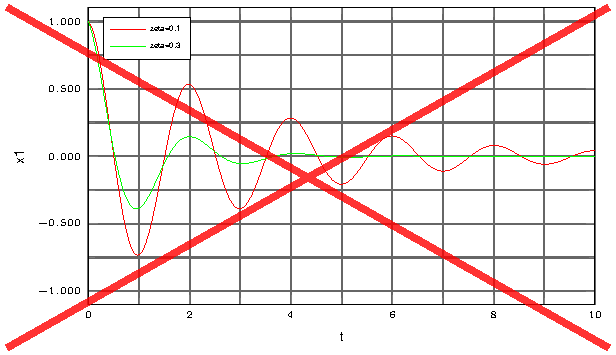
\includegraphics{PlotBad.pdf}
\caption{The damped oscillations of \cref{fig:goodplot}, plotted badly: hairline curves, a tiny legend over the data, fonts that do not match the text, curves told apart only by red and a pale pure green, axis labels without units, and a heavy grid.}
\label{fig:badplot}
\end{figure}

\begin{figure}
\centering
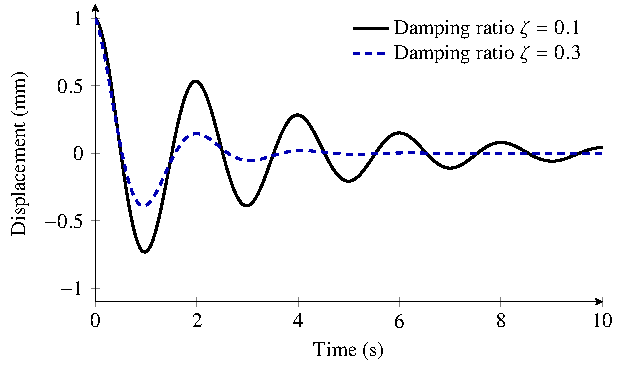
\includegraphics{PlotGood.pdf}
\caption{Displacement of a damped oscillator for two damping ratios, plotted well: thick curves in two line styles, a legible legend clear of the data, axis labels with units, and the Times font of the text at 10~pt.}
\label{fig:goodplot}
\end{figure}

Multiple sub-illustrations can be combined into a single floating figure using the \texttt{subfigure} environment provided by the \texttt{subcaption} package, as shown in \cref{fig:letters}.

\begin{figure}
\centering
\begin{subfigure}[b]{0.42\textwidth}
    \centering
    
\includegraphics[width=0.85\textwidth]{FancyA.jpg}
    \caption{Illuminated initial letter A.}
    \label{fig:letterA}
\end{subfigure}
\hfill
\begin{subfigure}[b]{0.42\textwidth}
    \centering
    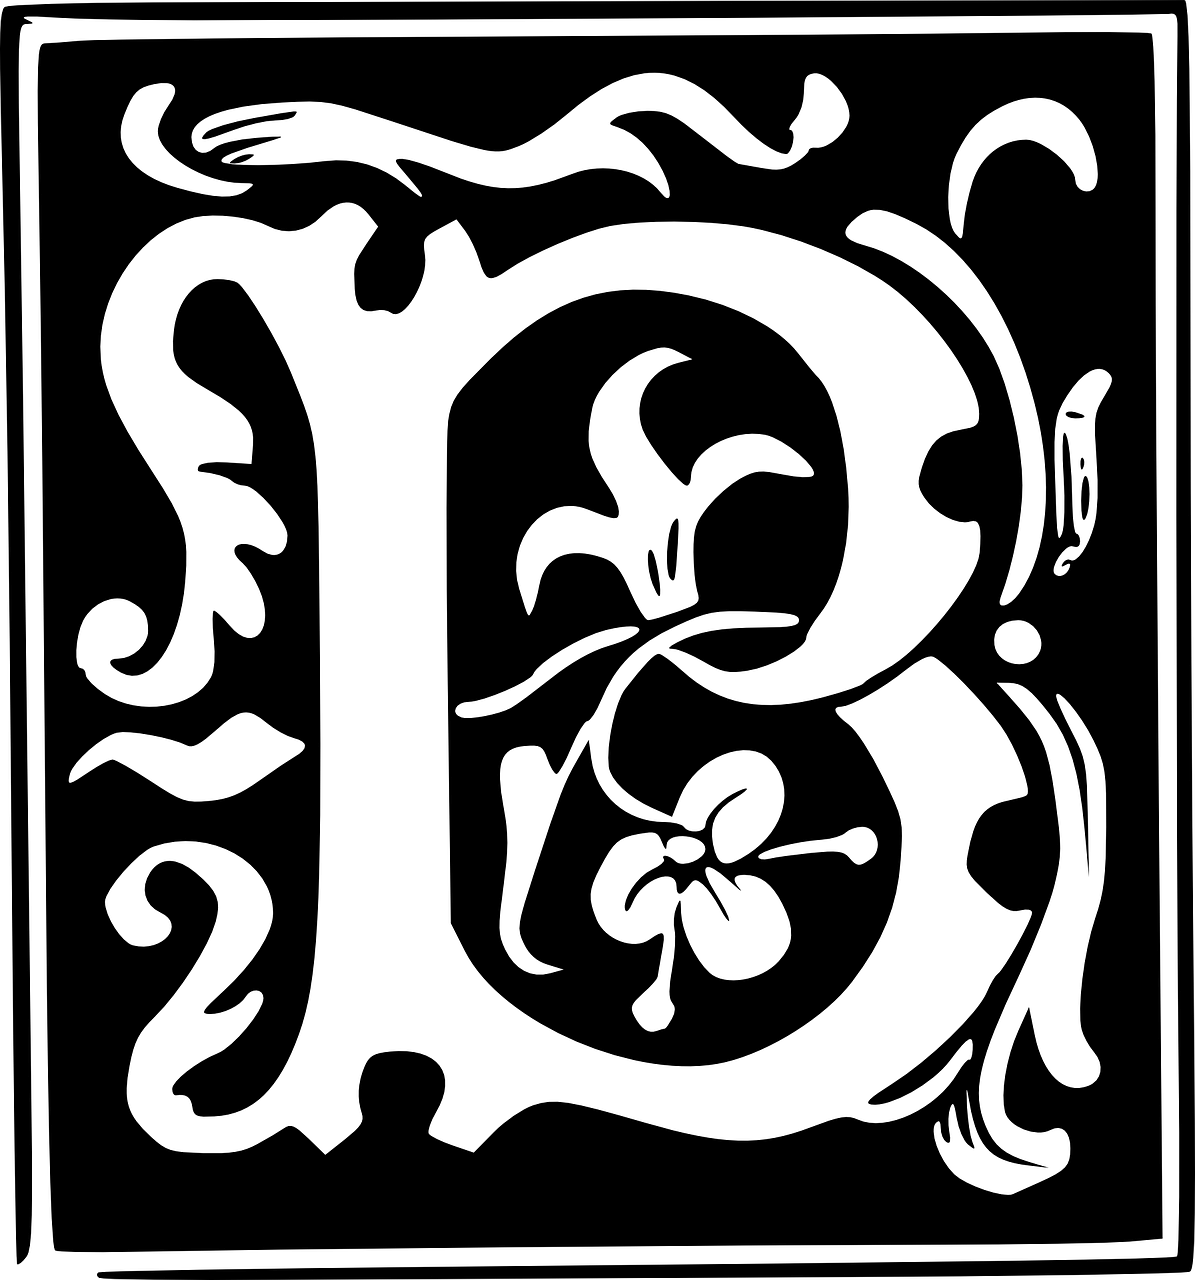
\includegraphics[width=0.85\textwidth]{FancyB.png}
    \caption{Illuminated initial letter B.}
    \label{fig:letterB}
\end{subfigure}
\caption{An example figure containing two subfigures, which may be referenced individually as \cref{fig:letterA} and \cref{fig:letterB}, or collectively as \cref{fig:letters}.}
\label{fig:letters}
\end{figure}

\section{Exporting Plots from MATLAB, Mathematica, and Python}
\label{sec:exportplots}

Save plots as vector PDF files whenever you can. A vector plot stays sharp at any magnification, and its text can be searched. Save photographs and other images as JPEG or PNG files with at least 300 pixels per inch at their printed size.

Make each plot at the size it will be printed, rather than scaling it in \LaTeX. If a plot drawn 8 inches wide is shrunk to 6 inches, its labels shrink by a quarter too. The text block is 6 inches wide, so a full-width plot should be about 6 inches wide, and each half of a two-part figure like \cref{fig:letters} about 3 inches. Then include it at its natural size, \verb+\includegraphics{plot.pdf}+, with no \texttt{width} option. Set the labels in a 10 or 11~pt font, and in Times if you can, so they match the text.
\begin{itemize}
\item \textbf{MATLAB}: Set the size and font, then save with \texttt{exportgraphics} (MATLAB R2020a or later):
\begin{verbatim}
fig = figure('Units','inches','Position',[1 1 6 4]);
plot(x, y);
set(gca, 'FontName','Times', 'FontSize',11);
exportgraphics(fig,'Graphics/plot.pdf','ContentType','vector');
\end{verbatim}
\item \textbf{Mathematica}: Give the width in printer's points (72 per inch) and export:
\begin{verbatim}
p = Plot[Sin[x], {x, 0, 2 Pi}, ImageSize -> 6*72,
      BaseStyle -> {FontFamily -> "Times", FontSize -> 11}];
Export["Graphics/plot.pdf", p]
\end{verbatim}
\item \textbf{Python (Matplotlib)}: Give the size in inches. The \texttt{pdf.fonttype} setting embeds the fonts as TrueType rather than Type~3 fonts, which some PDF checkers reject:
\begin{verbatim}
import matplotlib.pyplot as plt
plt.rcParams.update({"font.family": "serif",
    "font.serif": ["Times New Roman"], "font.size": 11,
    "pdf.fonttype": 42})
fig, ax = plt.subplots(figsize=(6, 4))
ax.plot(x, y)
fig.savefig("Graphics/plot.pdf")
\end{verbatim}
\end{itemize}

Another option is to draw the plot in \LaTeX\ itself with the \texttt{pgfplots} package, which sets the labels in the document's own fonts and accepts any \LaTeX\ math in them. It takes more work, and the package is not loaded by the template. MATLAB users can convert existing figures to \texttt{pgfplots} code with the \texttt{matlab2tikz} script. Whatever you use, check that the fonts in your figures are embedded in the final PDF (\cref{sec:checklist}).

\section{Using Figures You Did Not Create}
\label{sec:figurepermission}

Credit and permission are separate questions. Every figure, table, or algorithm you did not create needs a credit. Place the credit below the figure description or table, single-spaced. Type it with \verb+\floatsource+, followed by the reference in your chosen citation style, as in \cref{fig:eberhardt} and \cref{alg:bisection}. Some also need written permission from the copyright holder, because a dissertation is published, unlike a class paper.
\begin{itemize}
\item \textbf{No permission needed:} Works in the public domain, such as most images made by U.S.\ federal agencies, and works under a license that allows reuse, such as most Creative Commons licenses. Follow the license's terms for the credit line.
\item \textbf{Permission usually needed:} Figures copied from journal articles and books. Most publishers grant reuse in a dissertation quickly and without charge; look for a ``Rights and permissions'' link on the article's web page.
\item \textbf{Your own published papers:} Whether you may reuse a paper, or figures from it, depends on the agreement you signed with its publisher. Check the agreement for each paper. A reference librarian at the NJIT Library can help you work out what it allows.
\item \textbf{Redrawn figures:} A figure you redraw from someone else's design or data is still adapted from their work. It needs a credit, and it may need permission if it closely copies the original.
\end{itemize}
Typical credit lines are ``Reprinted from [12], with permission from Elsevier'' and ``Adapted from [12].'' Keep the permission letters or license records. If you are unsure whether you need permission, ask the NJIT Library before you submit.

\section{Tables}
\label{sec:tables}

According to NJIT style rules:
\begin{itemize}
\item Table titles are placed \textbf{above} the table.
\item Table titles are formatted in title case and do \textbf{not} end with a period.
\item The table text is single-spaced. It may be set in 10~pt type: put \verb+\footnotesize+ after \verb+\centering+ in the \texttt{table} environment.
\item Tables are numbered by chapter, like figures.
\item Do not split a table across pages if it fits on a single page (GSO). A floating \texttt{table} environment is never split: if the table does not fit in the space left on the page, \LaTeX\ moves it to the next page, or to a page of its own.
\item A table too long for one page must show ``\textbf{Table X.x (Continued)}'' in bold at the top of each page after the first (GSO). Set it with the \texttt{longtable} environment and put the class command \verb+\tablecontinued+ in its \verb+\endhead+ section, as in \cref{table:longsample}. The continued title is not listed again in the List of Tables.
\item The source of a table you did not create goes on a line below the table itself, not below its title, typed with \verb+\floatsource+ after the \texttt{tabular}.
\item The title appears word for word in the List of Tables.
\item Put the column units in the column header, not in every cell.
\end{itemize}

\subsection{Standard portrait table}
\cref{table:gso_rules}, in \cref{ch:requirements}, is a standard floating table in portrait mode. It is kept in its own file, \texttt{table.tex}, and pulled in with \verb+\input+. This is optional, but it keeps large tables, or tables generated by a script, out of the chapter text. The \texttt{booktabs} rules used in \cref{table:landscape_sample} (\verb+\toprule+, \verb+\midrule+, \verb+\bottomrule+, and no vertical lines) usually read more cleanly than the full grid of \cref{table:gso_rules}.

\subsection{Landscape orientation for wide tables}
\label{subsec:landscape}
Occasionally, a dissertation table or figure contains too many columns to fit within the standard 6-inch text width of a portrait page. The \texttt{njit\_thesis.cls} class includes built-in landscape capability via \texttt{pdflscape}. The \texttt{landscape} environment rotates the entire page content while keeping headers, footers, and page numbers in their proper orientation, and rotates the PDF page view so that it is easily readable on a screen without neck strain.

The GSO requires that on a landscape page the bottom of the table or figure faces the outer edge of the page, while the page number stays in its normal portrait position. The \texttt{landscape} environment does both.

\cref{table:landscape_sample}, in \cref{sec:checklist}, is a full landscape table. Its source in \texttt{chapter5.tex} shows how to set one up: put the \texttt{table} environment inside a \texttt{landscape} environment.

% !TEX root = main.tex
% Chapter 5: citing sources, citation styles, reference managers, the
% publications list, and the checklist before submitting.
%
% Each chapter lives in its own file, included from main.tex with \input.
% Start the file with \chapter{Title}; type the title in normal
% capitalization (the class sets it in capitals). Headings below it:
%   \section       level 2, Title Case
%   \subsection    level 3, sentence case
%   \subsubsection level 4, sentence case, run-in (the class adds the period)
%   \paragraph     level 5, sentence case, italic (the class adds the period)
% Every heading needs a title; an empty one stops the build with an error.

\chapter{References and Submission}
\label{ch:references}

This chapter explains how to cite sources and choose a citation style, how the publications list in the Biographical Sketch is built, and what to check before you send the document to the GSO.

\section{Citing Sources}
\label{sec:bibliography}

Bibliographic citations are managed by the modern \texttt{biblatex} package backed by \texttt{biber}. Citations in the text are inserted using the standard \verb+\cite+ command. The sample \texttt{references.bib} holds one entry of each common type, so you can copy the one you need: books~\cite{Lamport1994,Knuth1984,Mittelbach2023}, a journal article~\cite{KnuthPlass1981}, an article with many authors~\cite{Harris2020}, a chapter in a book~\cite{Halmos1973}, a Ph.D.\ dissertation~\cite{Adriazola2021}, software documentation~\cite{biblatex}, and a website~\cite{EberhardtWiki}. For a website, record the date the page was last updated in the \texttt{date} field and the date you consulted it in the \texttt{urldate} field; without a \texttt{date}, author-year styles print ``n.d.'' (no date). For software, give the version number and its release date.

Each \verb+\cite+ takes the key, or keys, of the entries in \texttt{references.bib}:
\begin{itemize}
\item \verb+\cite{KnuthPlass1981}+ gives \cite{KnuthPlass1981}, for one source;
\item \verb+\cite{Lamport1994,Knuth1984}+ gives \cite{Lamport1994,Knuth1984}, for several sources, with the keys separated by commas;
\item \verb+\cite[p.~23]{Lamport1994}+ gives \cite[p.~23]{Lamport1994}, for a specific page, given in square brackets before the key.
\end{itemize}
Put a tie before the citation, as in \verb+shown in~\cite{Halmos1973}+, so that it never starts a new line.

Some styles need other citation commands. In an author-year style, such as APA, ASCE, Chicago, Harvard, or TRB, \verb+\cite+ gives the authors and year without parentheses, so use \verb+\autocite+ for a citation in parentheses and \verb+\textcite+ when the authors are part of the sentence. In a style with superscript numbers, such as ACS, AIP, or AMA, a citation is not a word of the sentence, which changes how you write. Before you choose a style, read the Special Instructions on its page in \cref{app:citestyles}.

Choose a citation style that follows the conventions of your discipline (\cref{tab:phd-styles}), with your advisor, and select it by setting the \texttt{style=} option on the \texttt{biblatex} line in \texttt{packages.tex}; do not format references by hand. Whatever the style, the GSO asks that references be consistent in capitalization, punctuation, and format. Follow the rules of the style you choose, even where they differ from other styles: book titles are italic in most styles, for example, but not in Vancouver. If every entry follows the same style, your references will be consistent. The class sets each reference single-spaced, with a blank line between references.

Most formatting problems in a bibliography come from the \texttt{.bib} file, not from \LaTeX. When you copy entries from Google Scholar or a publisher:
\begin{itemize}
\item Type titles in title case, and protect capitals that must survive, such as proper names and acronyms, with braces, as in \verb+{Stability of {KdV} Solitons}+. A style that prints titles in sentence case lowers the other capitals for you, but no style can add capitals that are missing.
\item Check that author names are separated by \verb+and+, not commas.
\item Write journal names out in full, such as \emph{Journal of Fluid Mechanics} rather than \emph{J.\ Fluid Mech.} Publisher and Google Scholar entries often use abbreviations, so check the \verb+journal+ field of each entry.
\item Check every entry for missing volumes, pages, and years; the style cannot print what isn't there.
\end{itemize}

\section{Choosing a Citation Style}
\label{sec:citestyles}

Different fields of study have adopted different bibliography styles, which are conventions for formatting bibliography entries. \Cref{tab:phd-styles} lists the citation styles that each program recommends; some recommend several. The citation style is your choice, made with your advisor, based on the conventions in your discipline. The template gives you a working technical setup for each style; learn the style's rules from its official guide, listed in \cref{app:citestyles}.

The table of style codes in \texttt{packages.tex} gives the \texttt{style=} value for each style; Chicago is loaded differently, as the comment there explains. \texttt{biblatex} has no ACM, AIP, AMA, ASCE, or TRB style of its own, so the template supplies five: \texttt{njit-acm}, \texttt{njit-aip}, \texttt{njit-ama}, \texttt{njit-asce}, and \texttt{njit-trb}, in the files with those names in the template's main folder. ASCE and TRB citations give the author and year, as in their journals. The template's \texttt{njit-harvard} and \texttt{njit-vancouver} styles print titles in sentence case, as their guides ask, and \texttt{njit-vancouver} also separates all authors with commas, where \texttt{biblatex}'s own \texttt{vancouver} style puts ``and'' before the last one. AMA citations are superscript numbers that go after a period or comma; write \verb+as shown\autocite{Halmos1973}.+ and the period moves in front of the number. To compare the styles before you choose, see \cref{app:citestyles}: it shows every style in the table applied to the same sources, one style per page, with Special Instructions for the styles that need them.

\begin{table}
\centering
\caption{Citation Styles Recommended by Each Program}
\label{tab:phd-styles}
\begin{tabularx}{\linewidth}{>{\raggedright\arraybackslash}p{0.45\linewidth}X}
\toprule
\textbf{Program} & \textbf{Recommended Citation Styles} \\
\midrule
Applied Physics & ACS, AIP, Harvard \\
Biology & ACS \\
Biomedical Engineering & ACS, AMA, IEEE \\
Business Data Science & APA \\
Chemical Engineering & ACS, AIP, Chicago, Harvard \\
Chemistry & ACS \\
Civil Engineering & ACS, AIP, ASCE, Harvard, IEEE \\
Computer Engineering & IEEE \\
Computer Science & ACM, Chicago, IEEE \\
Data Science (Computing Option) & ACM, IEEE \\
Data Science (Statistics Option) & AMA, Chicago, Harvard, IEEE \\
Electrical Engineering & IEEE \\
Engineering Science & APA, IEEE \\
Environmental Engineering & ACS, AIP, ASCE, Chicago, Harvard \\
Environmental Science & APA \\
Industrial Engineering & APA, IEEE \\
Information Systems & ACM, APA \\
Materials Science and Engineering & ACS, AIP, Chicago, Harvard \\
Mathematical Sciences (Applied Mathematics Option) & AMS \\
Mathematical Sciences (Applied Probability and Statistics Option) & Chicago, Harvard, Vancouver \\
Mechanical Engineering & ACS, AIP, Chicago, Harvard, IEEE \\
Transportation & ACS, AIP, APA, ASCE, Chicago, IEEE, TRB \\
Urban Systems & APA \\
\bottomrule
\end{tabularx}
\end{table}

\section{Reference Managers}
\label{sec:refmanagers}
You don't have to type \texttt{.bib} entries by hand. A reference manager stores your sources, often together with their PDFs, and writes the \texttt{.bib} file for you.
\begin{itemize}
\item \textbf{Zotero} (free, all platforms) adds a source from a button in your web browser. With its Better BibTeX add-on, it keeps \texttt{references.bib} up to date as you add sources and gives every entry a stable citation key.
\item \textbf{JabRef} (free, all platforms) edits \texttt{.bib} files directly and can fetch an entry from a DOI or an arXiv number.
\item \textbf{BibDesk} (free, Mac only, included with MacTeX) also edits \texttt{.bib} files directly.
\item \textbf{Mendeley} and \textbf{EndNote} can export a \texttt{.bib} file.
\end{itemize}
Whichever you use, check the entries it produces against the list in \cref{sec:bibliography}. Reference managers copy abbreviated journal names and lowercase acronyms from their sources.

\section{The Publications List in the Biographical Sketch}
\label{sec:publist}
A major advantage of \texttt{biblatex} is its ability to produce multiple independent bibliographies. In this template, the Presentations and Publications listing in the Biographical Sketch is populated directly from the \texttt{references.bib} database by filtering for entries that include the tag:
\begin{verbatim}
keywords = {me},
\end{verbatim}
This eliminates the need to maintain two separate citation files. The publications you list in the Biographical Sketch must be formatted in the same style as the References (GSO), and because both lists come from \texttt{biblatex}, they automatically are.

\section{Before You Submit}
\label{sec:checklist}

Most documents the GSO returns have one of a handful of problems. Before you send yours, check that:
\begin{itemize}
\item You have run a spell-checker over the whole document, including the text in figures and tables.
\item The title is identical on the abstract, title, and approval pages (automatic if you set it only with \verb+\title+).
\item The Table of Contents and the Lists of Tables and Figures match the headings and captions in the text exactly.
\item The degree and department on the title page are a valid combination from the GSO's list, and the graduation month and year are correct.
\item Every figure, table, and appendix is referred to in the text.
\item The page numbers run without gaps, and there are no blank pages other than the one that replaces the copyright page in a master's thesis.
\item Every advisor and committee title has been checked against the current Graduate Catalog.
\item No cross-reference or citation shows as ``??''. Search the PDF for ``??'' to be sure.
\item The log file (\texttt{main.log}) has no overfull-box warnings that push text into the margin.
\item Every font in the PDF is embedded, including the fonts inside your figures. Open the PDF in Adobe Acrobat Reader, choose \emph{File}, then \emph{Properties}, then \emph{Fonts}, and check that each font is marked ``Embedded'' or ``Embedded Subset''. On the command line, \verb+pdffonts main.pdf+ (from the Poppler utilities) lists every font, with \texttt{yes} in the \texttt{emb} column for each embedded one. pdf\LaTeX\ embeds the fonts of the text itself, so a font that is not embedded almost always comes from a figure; export that figure again as described in \cref{sec:exportplots}.
\item The links work. Click a few entries in the Table of Contents, a few citations, and a few cross-references, and check that each one goes to the right place.
\end{itemize}

\cref{table:landscape_sample} lists the problems that most often cause the GSO to return a document, and how to avoid each one. It is also the sample's landscape table (\cref{subsec:landscape}).

\begin{landscape}
\begin{table}
\centering
\caption{Common Reasons the GSO Returns a Document and How to Avoid Them}
\label{table:landscape_sample}
\begin{tabularx}{\linewidth}{>{\raggedright\arraybackslash}p{0.2\linewidth}>{\raggedright\arraybackslash}X>{\raggedright\arraybackslash}X}
\toprule
\textbf{Problem} & \textbf{What the GSO Expects} & \textbf{How to Avoid It} \\
\midrule
Title differs between pages & The same title, word for word, on the abstract, title page, and approval page & Set it once with \texttt{\textbackslash title} in \texttt{biography.tex}; never retype it \\
\addlinespace[2pt]
Wrong degree, department, or date & A valid degree and department combination from the GSO list; the graduation month and year & Check the GSO list; set \texttt{\textbackslash graduationdate}, not the defense date \\
\addlinespace[2pt]
Faculty names or titles wrong & Names spelled correctly and titles as in the current Graduate Catalog & Confirm each one with your department administrator before filling in \texttt{approval.tex} \\
\addlinespace[2pt]
Committee too small & At least five members for a dissertation and three for a thesis, including the advisor; external members listed last & List members in \texttt{approval.tex} in that order \\
\addlinespace[2pt]
Lists do not match the text & Table of Contents and Lists of Tables and Figures identical to the headings and captions & Let \LaTeX\ generate them; do not give \texttt{\textbackslash caption} or headings a different short title in square brackets \\
\addlinespace[2pt]
Inconsistent capitalization & Level 2 headings and table titles in title case; levels 3 to 5 in sentence case & Type each heading in the right case; the class does not change it \\
\addlinespace[2pt]
Spelling and grammar errors & No errors anywhere, including text inside figures and tables & Spell-check the \texttt{.tex} files and proofread the labels in your figures \\
\addlinespace[2pt]
Missing references & No ``??'' in place of a citation or cross-reference & Compile until the log reports no undefined references; search the PDF for ``??'' \\
\addlinespace[2pt]
Text in the margin & Nothing extends past the margins & Fix every ``Overfull \textbackslash hbox'' warning in \texttt{main.log}, usually from wide equations, tables, or URLs \\
\addlinespace[2pt]
Abstract too long & One page for a thesis, two for a dissertation, in the third person & Check the length of the first page of the PDF \\
\addlinespace[2pt]
Appendix without introduction & Each appendix opens with a brief description before any figures or tables & Start every appendix with a paragraph of text \\
\bottomrule
\end{tabularx}
\end{table}
\end{landscape}


%%%%%%%%%%%%%%%%%%%%%%%%%%%%%%%%%%%%%%%%%%%%%%%%%%%%%%
%% Bibliography / References
%%%%%%%%%%%%%%%%%%%%%%%%%%%%%%%%%%%%%%%%%%%%%%%%%%%%%%
% The References come right after the last chapter, before all of the
% appendices (GSO).
\printbibliography[heading=bibintoc,title={REFERENCES}]

%%%%%%%%%%%%%%%%%%%%%%%%%%%%%%%%%%%%%%%%%%%%%%%%%%%%%%
%% Appendices
%%%%%%%%%%%%%%%%%%%%%%%%%%%%%%%%%%%%%%%%%%%%%%%%%%%%%%
\appendix

% --- Option A: Multiple Appendices (used by this sample) ---
% With TWO OR MORE appendices, input one file per appendix. Each file starts
% with \chapter{Title}; they are printed as APPENDIX A, APPENDIX B, ...
% !TEX root = main.tex
% APPENDIX A (one of several). Use appendixA.tex, appendixB.tex, ... when the
% document has TWO OR MORE appendices (they are lettered A, B, ...).
% Start each file with \chapter{Title}; \appendix in main.tex switches
% chapters to appendix lettering. Every appendix needs a title and a short
% introduction before any figures or tables (GSO).
% The sample text is shared with appendix.tex through appendix-rules.tex and
% appendix-demo.tex.

\chapter{Including an appendix or appendices}
\label{app:appendixA}

% !TEX root = main.tex
% Shared text: the GSO rules for appendices. Included with \input from both
% appendix.tex (single appendix) and appendixA.tex (several appendices), so
% the wording lives in one place. Your own appendices do not need
% this file.

An appendix holds material that supports the dissertation but that a reader does not need in order to follow the argument. A useful test: if a reader skipped the appendix, would the chapters still make sense and still support their conclusions? If not, the material belongs in a chapter.

\textbf{Keep in the chapters} everything a reader needs to follow and evaluate the work:
\begin{itemize}
\item the research questions, the methods, and the main results;
\item the figures and tables that present those results;
\item the key steps of the central proofs and derivations.
\end{itemize}

\textbf{Move to an appendix} material that is long, routine, or of interest mainly to a specialist checking the details:
\begin{itemize}
\item long or routine proofs and derivations, once the chapter has stated the result;
\item full data tables, when the chapter shows a summary;
\item additional figures that repeat a result for other parameters or cases;
\item survey instruments, interview protocols, and consent forms;
\item long source code or pseudocode;
\item details of experimental setups, calibrations, and numerical parameters.
\end{itemize}

Refer to every appendix from the chapter where its material is relevant, for example ``The full proof is given in Appendix~B.'' Material that no chapter refers to probably does not belong in the dissertation at all. Large data sets and complete software packages usually do not belong in an appendix either; upload them to ProQuest as Supplementary Files when you submit the dissertation, or deposit them in a public repository and cite them.

NJIT enforces a strict rule regarding the titling and numbering of appendices:
\begin{itemize}
\item If your dissertation has only a \textbf{single appendix}, it must be titled \textbf{APPENDIX} (without any letter label such as "A"), followed by the appendix title.
\item If your dissertation contains \textbf{two or more appendices}, they must be numbered sequentially as \textbf{APPENDIX A}, \textbf{APPENDIX B}, etc.
\end{itemize}

You should not try to format this manually. Instead:
\begin{itemize}
\item If you have \textbf{one} appendix, use \texttt{appendix.tex} and begin it with the command \verb+\oneappendix{Your Title}+. The heading prints as APPENDIX followed by your title in capitals.
\item If you have \textbf{two or more}, switch to the multi-appendix lines in \texttt{main.tex} and begin each file with \verb+\chapter{Your Title}+. They are lettered A, B, \ldots\ automatically.
\end{itemize}

Every appendix needs a title and a brief introductory description before any equations, figures, or tables (GSO). Appendix pages are numbered continuously with the chapters, and equations, figures, and tables in an appendix are numbered with the appendix letter, starting again at 1 (A.1, B.1, \ldots).


This sample has five appendices, so they are lettered: this is \textbf{APPENDIX A}, followed by \cref{app:citestyles}, which collects guides to the citation styles, \cref{app:packages}, which describes the packages the template loads, \cref{app:filetree}, which lists the template's files, and \cref{app:supplementary}, which lists supplementary files. The class file prints the letters in the headings and the Table of Contents and prefixes equations, theorems, figures, and tables with the letter, as the examples below show. To switch to a single, unlettered appendix, follow the instructions at the end of \texttt{main.tex}.

% !TEX root = main.tex
% Shared sample: demonstrates numbered equations, figures, and a table inside
% an appendix. Included with \input from appendix.tex (single appendix) and
% appendixA.tex (lettered appendices); only one of those is compiled at a
% time, so each label is defined once. Your own appendices do not
% need this file.

\section{Equations and Figures in Appendices}

Equations inside the appendix are numbered with an appendix prefix:
\begin{align}
\label{eq:app1}
\nabla^2 \phi - \frac{1}{c^2}\frac{\partial^2 \phi}{\partial t^2} &= 0, \\
\label{eq:app2}
\oint_{\partial \Omega} \mathbf{F} \cdot d\mathbf{S} &= \iiint_{\Omega} (\nabla \cdot \mathbf{F})\, dV.
\end{align}
Cross-references like \cref{eq:app1} and \cref{eq:app2} resolve cleanly.

Figures placed within the appendix also receive appropriate appendix numbering, as shown in \cref{fig:app_numeral1} and \cref{fig:app_numeral2}.

\begin{figure}
\centering
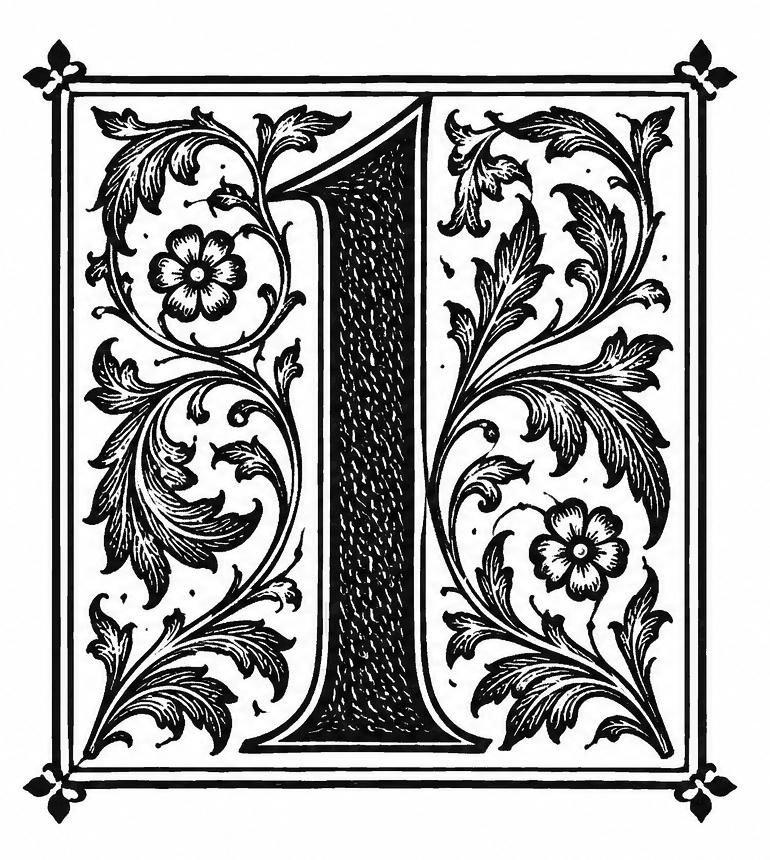
\includegraphics[width=2.5in]{drop_cap_1.png}
\caption{An ornamental numeral 1, the first appendix demonstration figure.}
\label{fig:app_numeral1}
\end{figure}

\begin{figure}
\centering
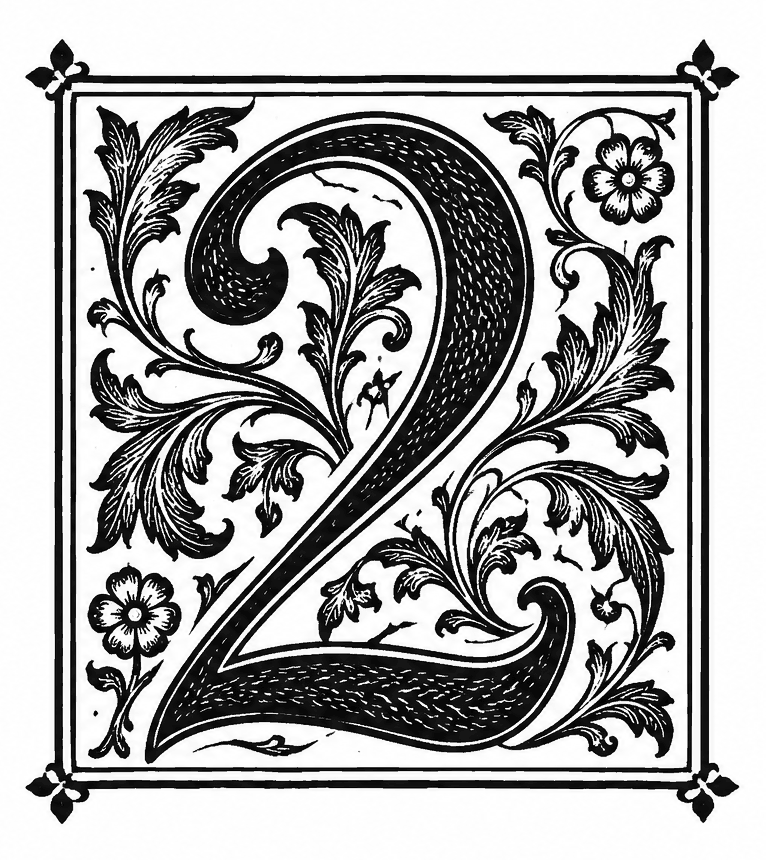
\includegraphics[width=2.5in]{drop_cap_2.png}
\caption{An ornamental numeral 2, the second appendix demonstration figure.}
\label{fig:app_numeral2}
\end{figure}

\section{Tables in an Appendix}

Here is an example of a table in an appendix showing how you might list websites you consulted. \cref{table:latexresources} lists free resources for learning \LaTeX\ and for answering questions as you write. The addresses are printed without the \texttt{https://} prefix, which keeps them short enough to fit the column, but each one still links to the full address:
\begin{verbatim}
\href{https://www.learnlatex.org}{\nolinkurl{www.learnlatex.org}}
\end{verbatim}
For an address printed in full, \verb+\url+ breaks long addresses at any character, thanks to the \texttt{xurl} package.

\begin{table}
\centering
\caption{Free Resources for Learning \LaTeX}
\label{table:latexresources}
\begin{tabularx}{\linewidth}{|>{\raggedright\arraybackslash}p{0.24\linewidth}|>{\raggedright\arraybackslash}p{0.36\linewidth}|>{\raggedright\arraybackslash}X|}
\hline
\textbf{Resource} & \textbf{Address} & \textbf{Good For} \\
\hline
Learn \LaTeX\ in 30 Minutes (Overleaf) & \href{https://www.overleaf.com/learn/latex/Learn_LaTeX_in_30_minutes}{\nolinkurl{www.overleaf.com/learn/latex/Learn_LaTeX_in_30_minutes}} & A first introduction, with examples you can edit online \\
\hline
learnlatex.org & \href{https://www.learnlatex.org}{\nolinkurl{www.learnlatex.org}} & Short interactive lessons covering the basics \\
\hline
Overleaf documentation & \href{https://www.overleaf.com/learn}{\nolinkurl{www.overleaf.com/learn}} & Task-based help on tables, figures, mathematics, and bibliographies \\
\hline
The Not So Short Introduction to \LaTeX & \href{https://ctan.org/pkg/lshort}{\nolinkurl{ctan.org/pkg/lshort}} & A complete free textbook \\
\hline
\LaTeX\ Wikibook & \href{https://en.wikibooks.org/wiki/LaTeX}{\nolinkurl{en.wikibooks.org/wiki/LaTeX}} & A searchable reference organized by topic \\
\hline
How Should We \LaTeX? (Roy Goodman) & \href{https://roygoodman.net/post/how-to-latex/}{\nolinkurl{roygoodman.net/post/how-to-latex}} & Style habits that manuals skip: meaningful macros, consistent notation, punctuating equations, and coauthoring \\
\hline
Short Math Guide for \LaTeX\ (AMS) & \href{https://ctan.org/pkg/short-math-guide}{\nolinkurl{ctan.org/pkg/short-math-guide}} & The commands of \texttt{amsmath} at a glance \\
\hline
Detexify & \href{https://detexify.kirelabs.org}{\nolinkurl{detexify.kirelabs.org}} & Finding the command for a symbol by drawing it \\
\hline
Comprehensive \LaTeX\ Symbol List & \href{https://ctan.org/pkg/comprehensive}{\nolinkurl{ctan.org/pkg/comprehensive}} & Every symbol available, with the package that provides it \\
\hline
TeX Stack Exchange & \href{https://tex.stackexchange.com}{\nolinkurl{tex.stackexchange.com}} & Answers to specific questions; search before asking \\
\hline
CTAN & \href{https://ctan.org}{\nolinkurl{ctan.org}} & Documentation for every package \\
\hline
\end{tabularx}
\end{table}

% \clearpage prints the floating Table A.1 first, so the tables stay in
% order; a longtable does not float and would otherwise come out first.
\clearpage
\section{Tables Longer Than One Page}

A table too long for one page is typed with the \texttt{longtable} environment instead of a \texttt{table} environment, as in \cref{table:longsample}. It does not float: it starts where it is typed and continues onto as many pages as it needs. Its title goes in the \verb+\endfirsthead+ part; the \verb+\endhead+ part, which starts with the class command \verb+\tablecontinued+, is repeated at the top of every later page, so each of them begins with ``\textbf{Table X.x (Continued)}'' and the column headings (GSO). The continued title is not listed again in the List of Tables.

\begin{longtable}{>{\centering\arraybackslash}p{0.15\linewidth}l>{\raggedright\arraybackslash}p{0.45\linewidth}}
\caption{Commands for Common Mathematical Symbols}
\label{table:longsample} \\
\toprule
\textbf{Symbol} & \textbf{Command} & \textbf{Meaning} \\
\midrule
\endfirsthead
\tablecontinued \\
\toprule
\textbf{Symbol} & \textbf{Command} & \textbf{Meaning} \\
\midrule
\endhead
\bottomrule
\endlastfoot
$\alpha$ & \verb+\alpha+ & Lowercase alpha \\
$\beta$ & \verb+\beta+ & Lowercase beta \\
$\gamma$ & \verb+\gamma+ & Lowercase gamma \\
$\delta$ & \verb+\delta+ & Lowercase delta \\
$\epsilon$ & \verb+\epsilon+ & Lowercase epsilon \\
$\zeta$ & \verb+\zeta+ & Lowercase zeta \\
$\eta$ & \verb+\eta+ & Lowercase eta \\
$\theta$ & \verb+\theta+ & Lowercase theta \\
$\iota$ & \verb+\iota+ & Lowercase iota \\
$\kappa$ & \verb+\kappa+ & Lowercase kappa \\
$\lambda$ & \verb+\lambda+ & Lowercase lambda \\
$\mu$ & \verb+\mu+ & Lowercase mu \\
$\nu$ & \verb+\nu+ & Lowercase nu \\
$\xi$ & \verb+\xi+ & Lowercase xi \\
$\pi$ & \verb+\pi+ & Lowercase pi \\
$\rho$ & \verb+\rho+ & Lowercase rho \\
$\sigma$ & \verb+\sigma+ & Lowercase sigma \\
$\tau$ & \verb+\tau+ & Lowercase tau \\
$\upsilon$ & \verb+\upsilon+ & Lowercase upsilon \\
$\phi$ & \verb+\phi+ & Lowercase phi \\
$\chi$ & \verb+\chi+ & Lowercase chi \\
$\psi$ & \verb+\psi+ & Lowercase psi \\
$\omega$ & \verb+\omega+ & Lowercase omega \\
$\varepsilon$ & \verb+\varepsilon+ & Variant of epsilon \\
$\vartheta$ & \verb+\vartheta+ & Variant of theta \\
$\varpi$ & \verb+\varpi+ & Variant of pi \\
$\varphi$ & \verb+\varphi+ & Variant of phi \\
$\Gamma$ & \verb+\Gamma+ & Uppercase gamma \\
$\Delta$ & \verb+\Delta+ & Uppercase delta \\
$\Theta$ & \verb+\Theta+ & Uppercase theta \\
$\Lambda$ & \verb+\Lambda+ & Uppercase lambda \\
$\Xi$ & \verb+\Xi+ & Uppercase xi \\
$\Pi$ & \verb+\Pi+ & Uppercase pi \\
$\Sigma$ & \verb+\Sigma+ & Uppercase sigma \\
$\Upsilon$ & \verb+\Upsilon+ & Uppercase upsilon \\
$\Phi$ & \verb+\Phi+ & Uppercase phi \\
$\Psi$ & \verb+\Psi+ & Uppercase psi \\
$\Omega$ & \verb+\Omega+ & Uppercase omega \\
$\nabla$ & \verb+\nabla+ & Gradient (nabla) \\
$\partial$ & \verb+\partial+ & Partial derivative \\
$\infty$ & \verb+\infty+ & Infinity \\
$\sum$ & \verb+\sum+ & Summation \\
$\prod$ & \verb+\prod+ & Product \\
$\int$ & \verb+\int+ & Integral \\
$\leq$ & \verb+\leq+ & Less than or equal to \\
$\geq$ & \verb+\geq+ & Greater than or equal to \\
$\neq$ & \verb+\neq+ & Not equal to \\
$\approx$ & \verb+\approx+ & Approximately equal to \\
$\in$ & \verb+\in+ & Element of \\
$\forall$ & \verb+\forall+ & For all \\
$\to$ & \verb+\to+ & Maps to, tends to \\
$\times$ & \verb+\times+ & Times, cross product \\
\end{longtable}


% !TEX root = main.tex
% APPENDIX B: the citation styles the programs recommend, with a sample page for
% each and a guide to each.
%
% biblatex allows only one citation style per document, so each sample
% page is a separate one-page document in the folder citation-styles/
% (style-acm.tex, style-acs.tex, ...). This appendix inserts their PDFs
% with \includepdf from the pdfpages package and prints the section
% heading over the space each page leaves blank at the top. The PDFs come
% with the template; to rebuild them after changing a style, run latexmk
% in the citation-styles folder.

% \stylesample{Name}{file} inserts citation-styles/style-file.pdf as a
% section of this appendix, with the heading, Table of Contents line, and
% page number of the thesis.
\newcommand{\stylesample}[2]{%
  \IfFileExists{citation-styles/style-#2.pdf}
    {\includepdf[pages=1,pagecommand={\thispagestyle{plain}%
       \section{#1}\label{sec:style-#2}}]{citation-styles/style-#2.pdf}}
    {\section{#1}\label{sec:style-#2}%
     The sample page for this style is missing. Run \texttt{latexmk} in the
     \texttt{citation-styles} folder to build it.\clearpage}}

\chapter{Citation styles}
\label{app:citestyles}

This appendix supports \cref{sec:citestyles}. \cref{tab:style-settings} lists the citation styles that the programs recommend (\cref{tab:phd-styles}) and how to select each one, and \cref{tab:style-resources} points to the official guide, or a reliable summary, for each. The citation style is your choice, made with your advisor, based on the conventions in your discipline; the template gives you a working technical setup for it, and the official guide teaches its rules. The sections that follow give each style one page. Each page lists the style's main distinguishing features and says how to type your sources in \texttt{references.bib} for it. It ends with the reference list the style produces from the same sources, in the same order, on every page: two books, a journal article, an article with many authors, a chapter in a book, a dissertation, software documentation, and a website. The citations are typed with \verb+\cite+, as in the rest of this sample. Some styles need another command or more care; their pages say so under Special Instructions, so read them before you choose.

Choose your citation style early, before you write much of the text, because the style changes how you write sentences that mention a source. In a style that cites with superscript numbers, such as AMA, or ACS and AIP when they cite with \verb+\autocite+, the number is not a word of the sentence: you cannot write ``In Reference\textsuperscript{5} it is shown that \ldots'' or ``as shown in\textsuperscript{5}''. You must name the authors instead, as in ``Knuth and Plass\textsuperscript{5} showed that \ldots''. In an author-year style, such as APA, Chicago, or Harvard, the authors' names are already part of the citation, and \verb+\textcite+ makes them part of the sentence: ``Knuth and Plass (1981) showed that \ldots''. Changing to a style of a different kind late in the work means rewriting these sentences by hand throughout the dissertation.

To use a style, set \texttt{style=} on the \texttt{biblatex} line in \texttt{packages.tex} to the value in \cref{tab:style-settings}, and compile the thesis again; nothing else changes. Chicago is the exception: replace the \texttt{biblatex} line as the comment in \texttt{packages.tex} shows. The ACM, AIP, AMA, ASCE, and TRB styles come with the template, because \texttt{biblatex} has none of its own. So do Harvard and Vancouver styles that capitalize titles as their guides ask; the Vancouver style also separates the authors with commas only.

A style can format only what is in \texttt{references.bib}. Type titles in title case and protect proper nouns and acronyms with braces, as in \texttt{\{NumPy\}}, so that styles which change capitalization keep them; write journal names out in full; and fill in every field a style needs. A style can change a title typed in title case to sentence case, but not the other way around, so title case works for every style. Each page repeats this advice and says what that style does to titles.

\begin{table}
\centering
\caption{Citation Styles and How to Select Them}
\label{tab:style-settings}
\begin{tabular}{@{}lll@{}}
\toprule
\textbf{Style} & \textbf{Setting in \texttt{packages.tex}} & \textbf{Citations in the Text} \\
\midrule
ACM       & \texttt{style=njit-acm}  & Numbers, [1] \\
ACS       & \texttt{style=chem-acs}  & Numbers, [1] or superscript \\
AIP       & \texttt{style=njit-aip}  & Numbers, [1] or superscript \\
AMA       & \texttt{style=njit-ama}  & Superscript numbers \\
AMS       & \texttt{style=alphabetic} & Labels, [KP81] \\
APA       & \texttt{style=apa}       & Author and year \\
ASCE      & \texttt{style=njit-asce} & Author and year \\
Chicago   & \texttt{biblatex-chicago} package & Author and year \\
Harvard   & \texttt{style=njit-harvard} & Author and year \\
IEEE      & \texttt{style=ieee}      & Numbers, [1] \\
TRB       & \texttt{style=njit-trb}  & Author and year \\
Vancouver & \texttt{style=njit-vancouver} & Numbers, [1] \\
\bottomrule
\end{tabular}
\end{table}

\begin{table}
\centering
\caption{Guides to the Citation Styles}
\label{tab:style-resources}
\begin{tabularx}{\linewidth}{>{\raggedright\arraybackslash}p{0.13\linewidth}>{\raggedright\arraybackslash}X}
\toprule
\textbf{Style} & \textbf{Resource} \\
\midrule
ACM & ACM reference formatting:\newline {\small\url{https://www.acm.org/publications/authors/reference-formatting}} \\
\addlinespace
ACS & ACS Guide to Scholarly Communication:\newline {\small\url{https://pubs.acs.org/books/pages/acsguide}} \\
\addlinespace
AIP & AIP Style Manual, 4th edition:\newline {\small\url{https://publishing.aip.org/wp-content/uploads/2021/03/AIP_Style_4thed.pdf}} \\
\addlinespace
AMA & Purdue OWL:\newline {\small\url{https://owl.purdue.edu/owl/research_and_citation/ama_style/index.html}} \\
\addlinespace
AMS & AMS Style Guide:\newline {\small\url{https://www.ams.org/publications/authors/AMS-StyleGuide-online.pdf}} \\
\addlinespace
APA & APA Style:\newline {\small\url{https://apastyle.apa.org}} \\
\addlinespace
ASCE & ASCE Library author center:\newline {\small\url{https://ascelibrary.org/author-center/preparing-manuscript}} \\
\addlinespace
Chicago & Purdue OWL:\newline {\small\url{https://owl.purdue.edu/owl/research_and_citation/chicago_manual_17th_edition/chicago_style_introduction.html}} \\
\addlinespace
Harvard & Open University:\newline {\small\url{https://university.open.ac.uk/library/referencing-and-plagiarism/quick-guide-to-harvard-referencing-cite-them-right}} \\
\addlinespace
IEEE & Purdue OWL:\newline {\small\url{https://owl.purdue.edu/owl/research_and_citation/ieee_style/ieee_overview.html}} \\
\addlinespace
TRB & Transportation Research Record author instructions:\newline {\small\url{https://trb.secure-platform.com/a/page/trrjournal/forauthors}} \\
\addlinespace
Vancouver & Purdue University Libraries:\newline {\small\url{https://guides.lib.purdue.edu/BMEQual/VancouverStyle}} \\
\bottomrule
\end{tabularx}
\end{table}

% Print the tables above before the first style page.
\clearpage
\stylesample{ACM}{acm}
\stylesample{ACS}{acs}
\stylesample{AIP}{aip}
\stylesample{AMA}{ama}
\stylesample{AMS}{ams}
\stylesample{APA}{apa}
\stylesample{ASCE}{asce}
\stylesample{Chicago}{chicago}
\stylesample{Harvard}{harvard}
\stylesample{IEEE}{ieee}
\stylesample{TRB}{trb}
\stylesample{Vancouver}{vancouver}

% !TEX root = main.tex
% APPENDIX C: describes the packages loaded in packages.tex. If you change
% packages.tex, update this appendix to match.

\chapter{Packages loaded by the template}
\label{app:packages}

Further information on each package, including its full documentation, is available at \url{https://ctan.org}, the Comprehensive \TeX\ Archive Network: search for the package by name. If compiling stops because a package is missing, see \cref{sec:missingpackages}.

This appendix lists every package loaded in \texttt{packages.tex}, in the order it is loaded, with the options the template chooses and why. Add packages your research needs in that file, before the \texttt{hyperref} line. Packages that the template needs for its layout are loaded by the class file itself and are listed in \cref{sec:classpackages}; you should not need to load those again.

\section{Packages in \texttt{packages.tex}}
\label{sec:packagestex}

\begin{itemize}
\item \texttt{fontenc}: Loaded with the option \texttt{T1}, which selects modern 8-bit font encoding. Accented letters then hyphenate correctly, and characters such as < and > print correctly in text.

\item \texttt{tabularx}: Provides the \texttt{tabularx} environment, whose \texttt{X} columns stretch to fill a given width. The sample tables use it to make tables exactly as wide as the text. It depends on \texttt{array}, which the class file loads (\cref{sec:classpackages}).

\item \texttt{booktabs}: Provides the horizontal rules \verb+\toprule+, \verb+\midrule+, and \verb+\bottomrule+, which give tables with better spacing than \verb+\hline+.

\item \texttt{amsmath}: The standard package for displayed mathematics: \texttt{align}, \texttt{gather}, \verb+\eqref+, \verb+\text+, and more. No options are needed.

\item \texttt{amsthm}: Provides \verb+\newtheorem+ styles and the \texttt{proof} environment. The theorem environments themselves are defined in \texttt{macros.tex}.

\item \texttt{mathtools}: Extends \texttt{amsmath} with fixes and additions such as \verb+\coloneqq+ and paired delimiters.

\item \texttt{newtxtext}: Sets the text in a Times clone (TeX Gyre Termes). The GSO requires Times New Roman or Arial at 12~pt.

\item \texttt{newtxmath}: Sets mathematics in fonts that match the Times text, and provides the AMS symbol fonts, so \texttt{amssymb} and \texttt{amsfonts} must \emph{not} be loaded as well. It must be loaded after \texttt{amsmath}.

\item \texttt{bm}: Provides \verb+\bm+, which makes any math symbol bold, as in the vector $\bm{p}$ in \cref{sec:math}. It is loaded after the math fonts so that it uses their bold versions.

\item \texttt{graphicx}: Provides \verb+\includegraphics+. Images are found in the \texttt{Graphics/} folder because \texttt{main.tex} sets \verb+\graphicspath{{Graphics/}}+.

\item \texttt{subcaption}: Provides the \texttt{subfigure} environment for figures with labelled parts (a), (b), and so on, as in \cref{fig:letters}. It works with the caption settings in the class.

\item \texttt{xurl}: Allows long URLs to break at any character, so URLs in tables and in the bibliography do not run into the margin.

\item \texttt{pdfpages}: Provides \verb+\includepdf+, which inserts pages of another PDF file. \cref{app:citestyles} uses it for the citation-style pages; you might use it for a signed form or a reprint, if your committee and the GSO allow it.

\item \texttt{csquotes}: Handles quotation marks. The command \verb+\MakeOuterQuote+ that follows it lets you type a straight double quote and get correct opening and closing quotation marks. It also makes that character special, so it can clash with some packages, such as \texttt{babel} shorthands for German.

\item \texttt{siunitx}: Typesets numbers and units consistently, with commands such as \verb+\qty+, \verb+\num+, and \verb+\unit+, and provides the \texttt{S} table column, which aligns numbers on the decimal point. See \cref{sec:math}. The template uses the commands of version~3, released in 2021.

\item \texttt{algorithm}: Provides the \texttt{algorithm} environment, which numbers an algorithm by chapter, sets its title above it between rules, and lists it in the List of Algorithms, as for \cref{alg:bisection}. The option \texttt{chapter} numbers algorithms within chapters, like figures and tables.

\item \texttt{algpseudocode}: Provides the \texttt{algorithmic} environment for the pseudocode inside an \texttt{algorithm} environment, as in \cref{alg:bisection}; it is part of the \texttt{algorithmicx} bundle. The two \verb+\renewcommand+ lines after it print ``Input:'' and ``Output:'' for \verb+\Require+ and \verb+\Ensure+.

\item \texttt{listings}: Typesets source code, as in \cref{sec:source_code}. The \verb+\lstset+ commands that follow it choose a small typewriter font, no line numbers, MATLAB as the default language, line breaking for long lines, blue keywords, red emphasis for a few control words, and dark green comments, which stay readable when printed. The colors come from \texttt{xcolor}, which the class file loads. Change \texttt{language} to match your own code.

\item \texttt{biblatex}: Formats citations and the bibliography, with \texttt{biber} as the back end. The option \texttt{style=numeric} sets the citation style; change it to one of the codes in the table of styles just above it in \texttt{packages.tex} (see \cref{sec:bibliography}). Five of those codes, \texttt{njit-acm}, \texttt{njit-aip}, \texttt{njit-ama}, \texttt{njit-asce}, and \texttt{njit-vancouver}, are styles that come with the template (see \cref{sec:filedescriptions}). The other options are:
  \texttt{backend=biber}, the program that processes \texttt{references.bib};
  \texttt{doi=false}, \texttt{url=false}, and \texttt{isbn=false}, which leave DOIs, URLs, and ISBNs out of the reference list (a URL still prints for an \texttt{@online} entry, or for any entry with the field \verb+options = {url=true}+);
  \texttt{giveninits=true}, which shortens given names to initials (\texttt{njit-acm} ignores it, because ACM spells out given names);
  \texttt{sortcites=true}, which sorts the numbers in a multiple citation, giving [1, 4, 5] rather than [5, 1, 4];
  and \texttt{defernums=true}, which assigns a number to an entry only when it is cited or printed, so entries in \texttt{references.bib} that are never used do not leave gaps in the numbering.
  The \verb+\defbibheading+ command after it gives the publications list in the Biographical Sketch an empty heading, because the class prints its own.

\item \texttt{hyperref}: Turns cross-references, citations, URLs, and Table of Contents entries into links, and adds PDF bookmarks. The option \texttt{hidelinks} keeps the links black and unboxed, so the printed copy is unchanged. It must be loaded after almost every other package, which is why it comes near the end.

\item \texttt{cleveref}: Provides \verb+\cref+, which prints the kind of item along with its number, such as ``Figure 2.1'' (see \cref{sec:crossrefs}). It must be loaded after \texttt{hyperref}. The option \texttt{capitalise} capitalizes the name everywhere, and \texttt{noabbrev} spells it out (``Equation'', not ``Eq.''). The \verb+\crefname+ line after it calls a subsection a ``Subsection''.
\end{itemize}

\section{Packages Loaded by the Class File}
\label{sec:classpackages}

The class file \texttt{njit\_thesis.cls} loads these packages itself, because the NJIT layout depends on them:
\begin{itemize}
\item \texttt{geometry}: Sets the 1.5-inch left margin and the 1-inch top, bottom, and right margins.
\item \texttt{setspace}: Double-spaces the text and single-spaces headings, captions, lists, and references.
\item \texttt{pdflscape}: Provides the \texttt{landscape} environment for landscape pages.
\item \texttt{caption}: Sets the caption layout: a bold label followed by two spaces and no colon, with table titles above the table and figure captions below the figure.
\item \texttt{etoolbox}: Provides the hooks the class uses internally.
\item \texttt{xcolor}: Defines colors by name. The class prints the titles of unnumbered sections in red, and the code listings in \texttt{packages.tex} use it for their colors.
\item \texttt{array}: Extends column specifications, for example \verb+>{\raggedright}p{2in}+ to set the alignment inside a paragraph column. \texttt{tabularx} depends on it.
\item \texttt{longtable}: Sets the two-column List of Symbols and Glossary of Terms, and tables too long for one page, such as \cref{table:longsample}, which can break across pages.
\end{itemize}

\section{If a Package Is Missing}
\label{sec:missingpackages}
The template loads a number of packages (listed in \cref{sec:packagestex,sec:classpackages}), and a \LaTeX\ installation does not necessarily include all of them. Overleaf and the \emph{full} installations of TeX Live, MacTeX, and MiKTeX include every package the template uses. Smaller installations, such as BasicTeX on a Mac or the \texttt{texlive-latex-base} package on Linux, do not.

A missing package stops the first \texttt{pdflatex} run with an error such as
\begin{verbatim}
! LaTeX Error: File `newtxtext.sty' not found.
\end{verbatim}
The file named in the message is what is missing; here it is \texttt{newtxtext.sty}. A missing \texttt{.cls}, \texttt{.bbx}, or \texttt{.cbx} file (a class or a \texttt{biblatex} style) is reported the same way. If the error instead says that \texttt{biber} could not be run or was not found, the \texttt{biber} program is missing, not a package. Stop the run (type \texttt{X} and press Enter, or close the log window in your editor) before installing anything.

A file and the package that contains it often have different names: \texttt{newtxtext.sty} belongs to the package \texttt{newtx}. To find the package name, search for the file name at \url{https://ctan.org}, or, with TeX Live or MacTeX, run
\begin{verbatim}
tlmgr search --global --file newtxtext.sty
\end{verbatim}

How to install the package depends on your \LaTeX\ distribution:
\begin{itemize}
\item \textbf{TeX Live (Windows or Linux) and MacTeX (Mac):} run \verb+tlmgr install newtx+, replacing \texttt{newtx} with the package name. On a Mac or Linux you will usually need \verb+sudo tlmgr install newtx+. On a Mac, the TeX Live Utility application does the same thing without the command line. The \texttt{biber} program installs the same way: \verb+tlmgr install biber+.
\item \textbf{TeX Live installed through a Linux package manager} (for example \texttt{apt} on Ubuntu or Debian): \texttt{tlmgr} may not work. Install the distribution package that contains the file instead; \verb+apt-file search newtxtext.sty+ names it (here, \texttt{texlive-fonts-extra}). Installing \texttt{texlive-full} avoids the problem altogether.
\item \textbf{MiKTeX (Windows):} MiKTeX normally offers to install a missing package the first time it is needed; accept the prompt. If it does not, open the MiKTeX Console, choose \emph{Packages}, search for the package, and install it.
\item \textbf{Overleaf:} nothing to install, since every package on CTAN is available.
\end{itemize}
Then compile again. If a different file is now reported missing, repeat these steps for it.

% !TEX root = main.tex
% APPENDIX D: the template's files. If you add or rename files, update the
% tree and the descriptions below.

\chapter{Files in the template}
\label{app:filetree}

The template is a folder of \LaTeX\ source files. Its main folder holds the class file, the shared settings, and the starter document in which you write your dissertation; the folder \texttt{sample/} holds this sample dissertation, which uses the class file and settings of the main folder. The tree below shows every file, grouped in the order \texttt{main.tex} reads them, and \cref{sec:filedescriptions} describes what each file contains.

{\setstretch{1}\footnotesize
\begin{verbatim}
NJIT-Thesis-Template/
|-- readme.md                Overview and build instructions
|-- LICENSE                  License (LPPL) for the class file
|-- njit_thesis.cls          Class file: the NJIT formatting rules
|-- packages.tex             Packages and citation style (Appendix C)
|-- njit-acm, njit-aip,      Citation styles (.bbx and .cbx):
|   njit-ama, njit-asce,       ACM, AIP, AMA, ASCE,
|   njit-harvard, njit-trb,    Harvard, TRB, and
|   njit-vancouver             Vancouver
|-- macros.tex               Your notation and theorem environments
|-- main.tex                 Starter document; write your thesis here
|-- references.bib           Your bibliography database
|-- abstract.tex             Front matter, in the order main.tex reads
|-- approval.tex               it; biography.tex also holds the title,
|-- biography.tex              name, degrees, and date
|-- acknowledgment.tex
|-- chapter1.tex             Chapter 1, with a table and a citation
|-- chapter2.tex             Chapter 2, with a figure
|-- appendix.tex             A single appendix
|-- Graphics/                Images for figures: PlotGood.pdf
`-- sample/                  This sample dissertation
    |-- main.tex             Its master file
    |-- references.bib       Sample bibliography database
    |-- abstract.tex, approval.tex, biography.tex,
    |   dedication.tex, acknowledgment.tex
    |-- listofsymbols.tex    Two-column List of Symbols
    |-- listofdefinitions.tex  Two-column Glossary of Terms
    |-- chapter1.tex         Chapter 1: getting started
    |-- chapter2.tex         Chapter 2: what the GSO requires
    |-- table.tex            Sample table, \input by chapter2.tex
    |-- chapter3.tex         Chapter 3: writing the text
    |-- chapter4.tex         Chapter 4: figures and tables
    |-- chapter5.tex         Chapter 5: references and submission
    |-- appendixA.tex        Appendix A (several appendices)
    |-- appendixB.tex        Appendix B: citation styles
    |-- appendixC.tex        Appendix C: packages
    |-- appendixD.tex        Appendix D: this list of files
    |-- appendix.tex         Alternative: a single appendix
    |-- supplementary.tex    List of supplementary files
    |-- appendix-rules.tex   Shared text, \input by appendix.tex
    |-- appendix-demo.tex      and appendixA.tex
    |-- Graphics/            Images for the sample's figures
    |       FancyA.jpg, FancyB.png, EberhardtHall.jpg,
    |       drop_cap_1.png, drop_cap_2.png,
    |       PlotBad.pdf, PlotGood.pdf, and their .tex sources
    `-- citation-styles/     The pages of Appendix B
        |-- style-page.tex   The page each style is applied to
        |-- style-acm.tex, ...  One file per style (12 in all),
        |-- style-acm.pdf, ...    and the page it produces
        `-- latexmkrc        Builds every page
\end{verbatim}
}

Compiling also creates \texttt{main.pdf} and a set of auxiliary files with the same base name (\texttt{main.aux}, \texttt{.bbl}, \texttt{.bcf}, \texttt{.blg}, \texttt{.fdb\_latexmk}, \texttt{.fls}, \texttt{.lof}, \texttt{.log}, \texttt{.lot}, \texttt{.run.xml}, \texttt{.synctex.gz}, and \texttt{.toc}). These are rebuilt on every run and can be deleted at any time.

\section{What Each File Contains}
\label{sec:filedescriptions}

Here is what each file contains and how to edit it. The files of the starter document and of this sample have the same names and the same roles; the starter's hold placeholder text.

\begin{itemize}
\emergencystretch=2.5em
  \item \texttt{njit\_thesis.cls}: The \LaTeX\ class file. It encapsulates all official NJIT Graduate Studies Office formatting rules, including 1.5-inch left margins for binding, 1.0-inch top/bottom/right margins, double line spacing for body text, centered bold uppercase chapter titles, multi-page continuation headers for the Table of Contents, Lists of Figures and Tables, and correct appendix handling. You should not need to edit this class file directly.

  \item \texttt{main.tex}: The master control document. It loads the class, includes packages and macros, sets the graphicspath, loads the front matter, and arranges the chapters and appendices via \verb+\input+ statements. The starter's \texttt{main.tex} has the optional parts (dedication, List of Algorithms, List of Symbols, Glossary of Terms) commented out; this sample's \texttt{sample/main.tex} uses all of them.

  \item \texttt{packages.tex}: Loads optional \LaTeX\ packages (such as \texttt{tabularx}, \texttt{amsmath}, \texttt{amsthm}, the Times fonts \texttt{newtxtext} and \texttt{newtxmath}, \texttt{graphicx}, \texttt{subcaption}, \texttt{booktabs}, \texttt{xurl}, and \texttt{biblatex}). Add any packages your research needs there, before the \texttt{hyperref} line.

  \item The \texttt{njit-*.bbx} and \texttt{njit-*.cbx} files: The ACM, AIP, AMA, ASCE, and TRB citation styles, which \texttt{biblatex} lacks, and Harvard and Vancouver styles that capitalize titles as their guides ask. Select one with \texttt{style=njit-acm}, \texttt{style=njit-harvard}, and so on, in \texttt{packages.tex}. The \texttt{.bbx} file formats the reference list and the \texttt{.cbx} file the citations; the comments at the top of each say what it does. \texttt{njit-acm} builds on the \texttt{acmnumeric} style of the \texttt{acmart} package, \texttt{njit-aip} on the \texttt{phys} style of \texttt{biblatex-phys}, \texttt{njit-asce}, \texttt{njit-harvard}, and \texttt{njit-trb} on the standard \texttt{authoryear} style, and \texttt{njit-vancouver} on the \texttt{vancouver} style of \texttt{biblatex-vancouver}; these packages come with every full \TeX\ installation and with Overleaf.

  \item \texttt{macros.tex}: Defines custom mathematical shortcuts and theorem environments (e.g., Theorem, Lemma, Definition, Proposition, Corollary). The file contains some examples. Well-defined and consistently used macros can make writing and editing your thesis much easier.

  \item \texttt{abstract.tex}: Enter the text of your abstract here. The class file automatically supplies the centered title and author header.

  \item \texttt{approval.tex}: Defines the dissertation advisor and committee members using the \verb+\advisor+ and \verb+\member+ commands. If you have a co-advisor, add \verb+\coadvisor{Name}{Title, Institution}+ after \verb+\advisor+; both advisors are then labeled ``Co-advisor'' and listed before the committee. Faculty titles must match the catalog.

  \item \texttt{biography.tex}: Contains your dissertation title, author name, major, degree title, department, institution, graduation date (\verb+\graduationdate+), and degrees earned (entered with the \verb+\degreeearned+ command; the older name \verb+\degree+ still works unless a package such as \texttt{gensymb} defines it). Also includes the hook for \verb+\printmypublications+.

  \item \texttt{dedication.tex}: Contains the optional dedication. The starter has none; to add one, copy \texttt{sample/dedication.tex} to the main folder and uncomment \verb+\dedication{% !TEX root = main.tex
% DEDICATION (optional; included via \dedication{% !TEX root = main.tex
% DEDICATION (optional; included via \dedication{\input{dedication}} in main.tex)
%
% A short dedication or quotation, set single-spaced in a centered block.
% Check the spelling of names and keep person and tense consistent (GSO).
% To omit the page, comment out the \dedication line in main.tex.
% Words left out of a quotation are marked with an ellipsis, typed \ldots;
% between two full sentences the first keeps its period (Chicago style).

\emph{Power of concentration is a very valuable quality, which few people acquire except through education. \ldots{} To be able to concentrate on the same matter for a considerable time is essential to difficult achievement, and even to the understanding of any complicated or abstruse subject.}

\begin{flushright}
Bertrand Russell, \emph{On Education} (1926)
\end{flushright}
} in main.tex)
%
% A short dedication or quotation, set single-spaced in a centered block.
% Check the spelling of names and keep person and tense consistent (GSO).
% To omit the page, comment out the \dedication line in main.tex.
% Words left out of a quotation are marked with an ellipsis, typed \ldots;
% between two full sentences the first keeps its period (Chicago style).

\emph{Power of concentration is a very valuable quality, which few people acquire except through education. \ldots{} To be able to concentrate on the same matter for a considerable time is essential to difficult achievement, and even to the understanding of any complicated or abstruse subject.}

\begin{flushright}
Bertrand Russell, \emph{On Education} (1926)
\end{flushright}
}+ in \texttt{main.tex}.

  \item \texttt{acknowledgment.tex}: Contains your acknowledgments. Thank your advisor first, then your committee; the GSO Front Matter guide then lists other contributors, family, funding sources, and technical support.

  \item \texttt{listofsymbols.tex}: Contains a two-column table of symbols and their meanings, one \verb+\sym{symbol}{meaning}+ per row. Included via \verb+\symbols+ in \texttt{main.tex}. Only in \texttt{sample/}; copy it to the main folder if you need it.

  \item \texttt{listofdefinitions.tex}: Contains a two-column table of terms and definitions in alphabetical order, one \verb+\term{term}{definition}+ per row. Included via \verb+\glossaryofterms+ in \texttt{main.tex}. Only in \texttt{sample/}, like the List of Symbols.


  \item \texttt{chapter1.tex}, \texttt{chapter2.tex}, \ldots: The individual chapter files. Keeping chapters in separate files allows you to comment out finished chapters while drafting new ones to speed up compilation. The starter has two, with a table in Chapter 1 and a figure in Chapter 2. The sample has five: getting started, what the GSO requires, writing the text, figures and tables, and references and submission.

  \item \texttt{table.tex}: The sample \cref{table:gso_rules}, kept in its own file and pulled into \texttt{chapter2.tex} with \verb+\input+, to show how a large or script-generated table can be kept out of the chapter text.

  \item \texttt{appendixA.tex} to \texttt{appendixD.tex}: The sample's four appendices, each starting with \verb+\chapter+: how appendices work, guides to the citation styles, the packages the template loads, and this list of files.

  \item \texttt{appendix.tex}: A single appendix, which starts with \verb+\oneappendix+ instead of \verb+\chapter+. The starter uses it; in this sample it is the alternative to \texttt{appendixA.tex}, switched in \texttt{sample/main.tex}. Sample text shared with \texttt{appendixA.tex} lives in \texttt{appendix-rules.tex} and \texttt{appendix-demo.tex}, pulled in with \verb+\input+.

  \item \texttt{supplementary.tex}: The list of supplementary files uploaded to ProQuest with the dissertation, which the GSO asks for as the last appendix (\cref{app:supplementary} here). It lists the files in a \texttt{supplementaryfiles} table. Only in \texttt{sample/}; copy it to the main folder, with the \verb+\input+ line from \texttt{sample/main.tex}, if you upload supplementary files.

  \item \texttt{references.bib}: A standard \BibTeX\ database of citations. Any entry with the field \verb+keywords = {me}+ will also be included automatically in the Presentations and Publications section of your Biographical Sketch. The starter's file holds one cited book and one placeholder paper of your own; the sample's has a model of each common entry type.

  \item \texttt{citation-styles/}: The pages of \cref{app:citestyles}, one for each citation style, each applying that style to the same sources from \texttt{references.bib}. \texttt{biblatex} allows only one citation style per document, so each page is a separate document, \texttt{style-acm.tex}, \texttt{style-acs.tex}, and so on, all laid out by \texttt{style-page.tex}; \cref{app:citestyles} inserts their PDFs with the \texttt{pdfpages} package. The PDFs come with the template. If you change \texttt{style-page.tex} or a style file, run \texttt{latexmk} in the folder with no file name to rebuild every page.

  \item \texttt{Graphics/}: Directory containing all figures, plots, and diagrams. The starter's holds the plot of \texttt{chapter2.tex}; the sample's, in \texttt{sample/Graphics/}, holds the images of this sample. If an image that a figure uses is missing, such as \texttt{EberhardtHall.jpg} for \cref{fig:eberhardt}, the sample prints a framed placeholder instead.
\end{itemize}


% Supplementary files (optional): only if you upload supplementary files
% (videos, data, software archives) to ProQuest. They are listed in the
% LAST appendix (GSO), which in this sample is Appendix E. To list them in
% your thesis, copy supplementary.tex and this line to ../main.tex.
% !TEX root = main.tex
% SUPPLEMENTARY FILES (included via % !TEX root = main.tex
% SUPPLEMENTARY FILES (included via % !TEX root = main.tex
% SUPPLEMENTARY FILES (included via \input{supplementary} in main.tex, as
% the last appendix).
%
% Files such as videos, data sets, and software archives can be uploaded to
% ProQuest as "Supplementary Files" along with the dissertation. If you
% upload any, the GSO asks that the dissertation list them in the LAST
% appendix, lettered like the others (Appendix E in this sample). Short
% sections of text, such as computer code, can be included in this
% appendix as well.
%
% List each file with \suppfile{file name}{description} in a
% supplementaryfiles table. Type an underscore in a file name as \_.
% If this is your only appendix, start it with
% \oneappendix{Supplementary Files} instead of \chapter, so that it is
% printed as "APPENDIX" with no letter.
%
% To list supplementary files in your thesis, copy this file to the main
% folder and add \input{supplementary} after your last appendix in
% ../main.tex.

\chapter{Supplementary Files}
\label{app:supplementary}

The following files were uploaded to ProQuest with this dissertation as supplementary files. Each description says what the file contains and which part of the dissertation it supports.

\begin{supplementaryfiles}
\suppfile{bisection\_demo.mp4}{A two-minute video of the bisection method (\cref{alg:bisection}) narrowing in on a root.}
\suppfile{wave\_solver.zip}{The MATLAB code used to compute the results in \cref{ch:figtables}, with instructions for running it in the file \texttt{README.txt}.}
\suppfile{symbol\_table.csv}{The data of \cref{table:longsample} as a comma-separated text file.}
\end{supplementaryfiles}
 in main.tex, as
% the last appendix).
%
% Files such as videos, data sets, and software archives can be uploaded to
% ProQuest as "Supplementary Files" along with the dissertation. If you
% upload any, the GSO asks that the dissertation list them in the LAST
% appendix, lettered like the others (Appendix E in this sample). Short
% sections of text, such as computer code, can be included in this
% appendix as well.
%
% List each file with \suppfile{file name}{description} in a
% supplementaryfiles table. Type an underscore in a file name as \_.
% If this is your only appendix, start it with
% \oneappendix{Supplementary Files} instead of \chapter, so that it is
% printed as "APPENDIX" with no letter.
%
% To list supplementary files in your thesis, copy this file to the main
% folder and add % !TEX root = main.tex
% SUPPLEMENTARY FILES (included via \input{supplementary} in main.tex, as
% the last appendix).
%
% Files such as videos, data sets, and software archives can be uploaded to
% ProQuest as "Supplementary Files" along with the dissertation. If you
% upload any, the GSO asks that the dissertation list them in the LAST
% appendix, lettered like the others (Appendix E in this sample). Short
% sections of text, such as computer code, can be included in this
% appendix as well.
%
% List each file with \suppfile{file name}{description} in a
% supplementaryfiles table. Type an underscore in a file name as \_.
% If this is your only appendix, start it with
% \oneappendix{Supplementary Files} instead of \chapter, so that it is
% printed as "APPENDIX" with no letter.
%
% To list supplementary files in your thesis, copy this file to the main
% folder and add \input{supplementary} after your last appendix in
% ../main.tex.

\chapter{Supplementary Files}
\label{app:supplementary}

The following files were uploaded to ProQuest with this dissertation as supplementary files. Each description says what the file contains and which part of the dissertation it supports.

\begin{supplementaryfiles}
\suppfile{bisection\_demo.mp4}{A two-minute video of the bisection method (\cref{alg:bisection}) narrowing in on a root.}
\suppfile{wave\_solver.zip}{The MATLAB code used to compute the results in \cref{ch:figtables}, with instructions for running it in the file \texttt{README.txt}.}
\suppfile{symbol\_table.csv}{The data of \cref{table:longsample} as a comma-separated text file.}
\end{supplementaryfiles}
 after your last appendix in
% ../main.tex.

\chapter{Supplementary Files}
\label{app:supplementary}

The following files were uploaded to ProQuest with this dissertation as supplementary files. Each description says what the file contains and which part of the dissertation it supports.

\begin{supplementaryfiles}
\suppfile{bisection\_demo.mp4}{A two-minute video of the bisection method (\cref{alg:bisection}) narrowing in on a root.}
\suppfile{wave\_solver.zip}{The MATLAB code used to compute the results in \cref{ch:figtables}, with instructions for running it in the file \texttt{README.txt}.}
\suppfile{symbol\_table.csv}{The data of \cref{table:longsample} as a comma-separated text file.}
\end{supplementaryfiles}
 in main.tex, as
% the last appendix).
%
% Files such as videos, data sets, and software archives can be uploaded to
% ProQuest as "Supplementary Files" along with the dissertation. If you
% upload any, the GSO asks that the dissertation list them in the LAST
% appendix, lettered like the others (Appendix E in this sample). Short
% sections of text, such as computer code, can be included in this
% appendix as well.
%
% List each file with \suppfile{file name}{description} in a
% supplementaryfiles table. Type an underscore in a file name as \_.
% If this is your only appendix, start it with
% \oneappendix{Supplementary Files} instead of \chapter, so that it is
% printed as "APPENDIX" with no letter.
%
% To list supplementary files in your thesis, copy this file to the main
% folder and add % !TEX root = main.tex
% SUPPLEMENTARY FILES (included via % !TEX root = main.tex
% SUPPLEMENTARY FILES (included via \input{supplementary} in main.tex, as
% the last appendix).
%
% Files such as videos, data sets, and software archives can be uploaded to
% ProQuest as "Supplementary Files" along with the dissertation. If you
% upload any, the GSO asks that the dissertation list them in the LAST
% appendix, lettered like the others (Appendix E in this sample). Short
% sections of text, such as computer code, can be included in this
% appendix as well.
%
% List each file with \suppfile{file name}{description} in a
% supplementaryfiles table. Type an underscore in a file name as \_.
% If this is your only appendix, start it with
% \oneappendix{Supplementary Files} instead of \chapter, so that it is
% printed as "APPENDIX" with no letter.
%
% To list supplementary files in your thesis, copy this file to the main
% folder and add \input{supplementary} after your last appendix in
% ../main.tex.

\chapter{Supplementary Files}
\label{app:supplementary}

The following files were uploaded to ProQuest with this dissertation as supplementary files. Each description says what the file contains and which part of the dissertation it supports.

\begin{supplementaryfiles}
\suppfile{bisection\_demo.mp4}{A two-minute video of the bisection method (\cref{alg:bisection}) narrowing in on a root.}
\suppfile{wave\_solver.zip}{The MATLAB code used to compute the results in \cref{ch:figtables}, with instructions for running it in the file \texttt{README.txt}.}
\suppfile{symbol\_table.csv}{The data of \cref{table:longsample} as a comma-separated text file.}
\end{supplementaryfiles}
 in main.tex, as
% the last appendix).
%
% Files such as videos, data sets, and software archives can be uploaded to
% ProQuest as "Supplementary Files" along with the dissertation. If you
% upload any, the GSO asks that the dissertation list them in the LAST
% appendix, lettered like the others (Appendix E in this sample). Short
% sections of text, such as computer code, can be included in this
% appendix as well.
%
% List each file with \suppfile{file name}{description} in a
% supplementaryfiles table. Type an underscore in a file name as \_.
% If this is your only appendix, start it with
% \oneappendix{Supplementary Files} instead of \chapter, so that it is
% printed as "APPENDIX" with no letter.
%
% To list supplementary files in your thesis, copy this file to the main
% folder and add % !TEX root = main.tex
% SUPPLEMENTARY FILES (included via \input{supplementary} in main.tex, as
% the last appendix).
%
% Files such as videos, data sets, and software archives can be uploaded to
% ProQuest as "Supplementary Files" along with the dissertation. If you
% upload any, the GSO asks that the dissertation list them in the LAST
% appendix, lettered like the others (Appendix E in this sample). Short
% sections of text, such as computer code, can be included in this
% appendix as well.
%
% List each file with \suppfile{file name}{description} in a
% supplementaryfiles table. Type an underscore in a file name as \_.
% If this is your only appendix, start it with
% \oneappendix{Supplementary Files} instead of \chapter, so that it is
% printed as "APPENDIX" with no letter.
%
% To list supplementary files in your thesis, copy this file to the main
% folder and add \input{supplementary} after your last appendix in
% ../main.tex.

\chapter{Supplementary Files}
\label{app:supplementary}

The following files were uploaded to ProQuest with this dissertation as supplementary files. Each description says what the file contains and which part of the dissertation it supports.

\begin{supplementaryfiles}
\suppfile{bisection\_demo.mp4}{A two-minute video of the bisection method (\cref{alg:bisection}) narrowing in on a root.}
\suppfile{wave\_solver.zip}{The MATLAB code used to compute the results in \cref{ch:figtables}, with instructions for running it in the file \texttt{README.txt}.}
\suppfile{symbol\_table.csv}{The data of \cref{table:longsample} as a comma-separated text file.}
\end{supplementaryfiles}
 after your last appendix in
% ../main.tex.

\chapter{Supplementary Files}
\label{app:supplementary}

The following files were uploaded to ProQuest with this dissertation as supplementary files. Each description says what the file contains and which part of the dissertation it supports.

\begin{supplementaryfiles}
\suppfile{bisection\_demo.mp4}{A two-minute video of the bisection method (\cref{alg:bisection}) narrowing in on a root.}
\suppfile{wave\_solver.zip}{The MATLAB code used to compute the results in \cref{ch:figtables}, with instructions for running it in the file \texttt{README.txt}.}
\suppfile{symbol\_table.csv}{The data of \cref{table:longsample} as a comma-separated text file.}
\end{supplementaryfiles}
 after your last appendix in
% ../main.tex.

\chapter{Supplementary Files}
\label{app:supplementary}

The following files were uploaded to ProQuest with this dissertation as supplementary files. Each description says what the file contains and which part of the dissertation it supports.

\begin{supplementaryfiles}
\suppfile{bisection\_demo.mp4}{A two-minute video of the bisection method (\cref{alg:bisection}) narrowing in on a root.}
\suppfile{wave\_solver.zip}{The MATLAB code used to compute the results in \cref{ch:figtables}, with instructions for running it in the file \texttt{README.txt}.}
\suppfile{symbol\_table.csv}{The data of \cref{table:longsample} as a comma-separated text file.}
\end{supplementaryfiles}


% --- Option B: Single Appendix ---
% With only ONE appendix, comment out the \input lines above and uncomment
% the line below. appendix.tex starts with \oneappendix{Title}, which prints the
% heading as "APPENDIX" with no letter, as NJIT requires. If your only
% appendix lists supplementary files, keep % !TEX root = main.tex
% SUPPLEMENTARY FILES (included via % !TEX root = main.tex
% SUPPLEMENTARY FILES (included via % !TEX root = main.tex
% SUPPLEMENTARY FILES (included via \input{supplementary} in main.tex, as
% the last appendix).
%
% Files such as videos, data sets, and software archives can be uploaded to
% ProQuest as "Supplementary Files" along with the dissertation. If you
% upload any, the GSO asks that the dissertation list them in the LAST
% appendix, lettered like the others (Appendix E in this sample). Short
% sections of text, such as computer code, can be included in this
% appendix as well.
%
% List each file with \suppfile{file name}{description} in a
% supplementaryfiles table. Type an underscore in a file name as \_.
% If this is your only appendix, start it with
% \oneappendix{Supplementary Files} instead of \chapter, so that it is
% printed as "APPENDIX" with no letter.
%
% To list supplementary files in your thesis, copy this file to the main
% folder and add \input{supplementary} after your last appendix in
% ../main.tex.

\chapter{Supplementary Files}
\label{app:supplementary}

The following files were uploaded to ProQuest with this dissertation as supplementary files. Each description says what the file contains and which part of the dissertation it supports.

\begin{supplementaryfiles}
\suppfile{bisection\_demo.mp4}{A two-minute video of the bisection method (\cref{alg:bisection}) narrowing in on a root.}
\suppfile{wave\_solver.zip}{The MATLAB code used to compute the results in \cref{ch:figtables}, with instructions for running it in the file \texttt{README.txt}.}
\suppfile{symbol\_table.csv}{The data of \cref{table:longsample} as a comma-separated text file.}
\end{supplementaryfiles}
 in main.tex, as
% the last appendix).
%
% Files such as videos, data sets, and software archives can be uploaded to
% ProQuest as "Supplementary Files" along with the dissertation. If you
% upload any, the GSO asks that the dissertation list them in the LAST
% appendix, lettered like the others (Appendix E in this sample). Short
% sections of text, such as computer code, can be included in this
% appendix as well.
%
% List each file with \suppfile{file name}{description} in a
% supplementaryfiles table. Type an underscore in a file name as \_.
% If this is your only appendix, start it with
% \oneappendix{Supplementary Files} instead of \chapter, so that it is
% printed as "APPENDIX" with no letter.
%
% To list supplementary files in your thesis, copy this file to the main
% folder and add % !TEX root = main.tex
% SUPPLEMENTARY FILES (included via \input{supplementary} in main.tex, as
% the last appendix).
%
% Files such as videos, data sets, and software archives can be uploaded to
% ProQuest as "Supplementary Files" along with the dissertation. If you
% upload any, the GSO asks that the dissertation list them in the LAST
% appendix, lettered like the others (Appendix E in this sample). Short
% sections of text, such as computer code, can be included in this
% appendix as well.
%
% List each file with \suppfile{file name}{description} in a
% supplementaryfiles table. Type an underscore in a file name as \_.
% If this is your only appendix, start it with
% \oneappendix{Supplementary Files} instead of \chapter, so that it is
% printed as "APPENDIX" with no letter.
%
% To list supplementary files in your thesis, copy this file to the main
% folder and add \input{supplementary} after your last appendix in
% ../main.tex.

\chapter{Supplementary Files}
\label{app:supplementary}

The following files were uploaded to ProQuest with this dissertation as supplementary files. Each description says what the file contains and which part of the dissertation it supports.

\begin{supplementaryfiles}
\suppfile{bisection\_demo.mp4}{A two-minute video of the bisection method (\cref{alg:bisection}) narrowing in on a root.}
\suppfile{wave\_solver.zip}{The MATLAB code used to compute the results in \cref{ch:figtables}, with instructions for running it in the file \texttt{README.txt}.}
\suppfile{symbol\_table.csv}{The data of \cref{table:longsample} as a comma-separated text file.}
\end{supplementaryfiles}
 after your last appendix in
% ../main.tex.

\chapter{Supplementary Files}
\label{app:supplementary}

The following files were uploaded to ProQuest with this dissertation as supplementary files. Each description says what the file contains and which part of the dissertation it supports.

\begin{supplementaryfiles}
\suppfile{bisection\_demo.mp4}{A two-minute video of the bisection method (\cref{alg:bisection}) narrowing in on a root.}
\suppfile{wave\_solver.zip}{The MATLAB code used to compute the results in \cref{ch:figtables}, with instructions for running it in the file \texttt{README.txt}.}
\suppfile{symbol\_table.csv}{The data of \cref{table:longsample} as a comma-separated text file.}
\end{supplementaryfiles}
 in main.tex, as
% the last appendix).
%
% Files such as videos, data sets, and software archives can be uploaded to
% ProQuest as "Supplementary Files" along with the dissertation. If you
% upload any, the GSO asks that the dissertation list them in the LAST
% appendix, lettered like the others (Appendix E in this sample). Short
% sections of text, such as computer code, can be included in this
% appendix as well.
%
% List each file with \suppfile{file name}{description} in a
% supplementaryfiles table. Type an underscore in a file name as \_.
% If this is your only appendix, start it with
% \oneappendix{Supplementary Files} instead of \chapter, so that it is
% printed as "APPENDIX" with no letter.
%
% To list supplementary files in your thesis, copy this file to the main
% folder and add % !TEX root = main.tex
% SUPPLEMENTARY FILES (included via % !TEX root = main.tex
% SUPPLEMENTARY FILES (included via \input{supplementary} in main.tex, as
% the last appendix).
%
% Files such as videos, data sets, and software archives can be uploaded to
% ProQuest as "Supplementary Files" along with the dissertation. If you
% upload any, the GSO asks that the dissertation list them in the LAST
% appendix, lettered like the others (Appendix E in this sample). Short
% sections of text, such as computer code, can be included in this
% appendix as well.
%
% List each file with \suppfile{file name}{description} in a
% supplementaryfiles table. Type an underscore in a file name as \_.
% If this is your only appendix, start it with
% \oneappendix{Supplementary Files} instead of \chapter, so that it is
% printed as "APPENDIX" with no letter.
%
% To list supplementary files in your thesis, copy this file to the main
% folder and add \input{supplementary} after your last appendix in
% ../main.tex.

\chapter{Supplementary Files}
\label{app:supplementary}

The following files were uploaded to ProQuest with this dissertation as supplementary files. Each description says what the file contains and which part of the dissertation it supports.

\begin{supplementaryfiles}
\suppfile{bisection\_demo.mp4}{A two-minute video of the bisection method (\cref{alg:bisection}) narrowing in on a root.}
\suppfile{wave\_solver.zip}{The MATLAB code used to compute the results in \cref{ch:figtables}, with instructions for running it in the file \texttt{README.txt}.}
\suppfile{symbol\_table.csv}{The data of \cref{table:longsample} as a comma-separated text file.}
\end{supplementaryfiles}
 in main.tex, as
% the last appendix).
%
% Files such as videos, data sets, and software archives can be uploaded to
% ProQuest as "Supplementary Files" along with the dissertation. If you
% upload any, the GSO asks that the dissertation list them in the LAST
% appendix, lettered like the others (Appendix E in this sample). Short
% sections of text, such as computer code, can be included in this
% appendix as well.
%
% List each file with \suppfile{file name}{description} in a
% supplementaryfiles table. Type an underscore in a file name as \_.
% If this is your only appendix, start it with
% \oneappendix{Supplementary Files} instead of \chapter, so that it is
% printed as "APPENDIX" with no letter.
%
% To list supplementary files in your thesis, copy this file to the main
% folder and add % !TEX root = main.tex
% SUPPLEMENTARY FILES (included via \input{supplementary} in main.tex, as
% the last appendix).
%
% Files such as videos, data sets, and software archives can be uploaded to
% ProQuest as "Supplementary Files" along with the dissertation. If you
% upload any, the GSO asks that the dissertation list them in the LAST
% appendix, lettered like the others (Appendix E in this sample). Short
% sections of text, such as computer code, can be included in this
% appendix as well.
%
% List each file with \suppfile{file name}{description} in a
% supplementaryfiles table. Type an underscore in a file name as \_.
% If this is your only appendix, start it with
% \oneappendix{Supplementary Files} instead of \chapter, so that it is
% printed as "APPENDIX" with no letter.
%
% To list supplementary files in your thesis, copy this file to the main
% folder and add \input{supplementary} after your last appendix in
% ../main.tex.

\chapter{Supplementary Files}
\label{app:supplementary}

The following files were uploaded to ProQuest with this dissertation as supplementary files. Each description says what the file contains and which part of the dissertation it supports.

\begin{supplementaryfiles}
\suppfile{bisection\_demo.mp4}{A two-minute video of the bisection method (\cref{alg:bisection}) narrowing in on a root.}
\suppfile{wave\_solver.zip}{The MATLAB code used to compute the results in \cref{ch:figtables}, with instructions for running it in the file \texttt{README.txt}.}
\suppfile{symbol\_table.csv}{The data of \cref{table:longsample} as a comma-separated text file.}
\end{supplementaryfiles}
 after your last appendix in
% ../main.tex.

\chapter{Supplementary Files}
\label{app:supplementary}

The following files were uploaded to ProQuest with this dissertation as supplementary files. Each description says what the file contains and which part of the dissertation it supports.

\begin{supplementaryfiles}
\suppfile{bisection\_demo.mp4}{A two-minute video of the bisection method (\cref{alg:bisection}) narrowing in on a root.}
\suppfile{wave\_solver.zip}{The MATLAB code used to compute the results in \cref{ch:figtables}, with instructions for running it in the file \texttt{README.txt}.}
\suppfile{symbol\_table.csv}{The data of \cref{table:longsample} as a comma-separated text file.}
\end{supplementaryfiles}
 after your last appendix in
% ../main.tex.

\chapter{Supplementary Files}
\label{app:supplementary}

The following files were uploaded to ProQuest with this dissertation as supplementary files. Each description says what the file contains and which part of the dissertation it supports.

\begin{supplementaryfiles}
\suppfile{bisection\_demo.mp4}{A two-minute video of the bisection method (\cref{alg:bisection}) narrowing in on a root.}
\suppfile{wave\_solver.zip}{The MATLAB code used to compute the results in \cref{ch:figtables}, with instructions for running it in the file \texttt{README.txt}.}
\suppfile{symbol\_table.csv}{The data of \cref{table:longsample} as a comma-separated text file.}
\end{supplementaryfiles}
 instead of
% this line and change \chapter to \oneappendix in supplementary.tex.
%% !TEX root = main.tex
% SINGLE APPENDIX. Use this file when the document has exactly ONE appendix
% (it is printed as "APPENDIX", with no letter). Start with
% \oneappendix{Title}. For two or more appendices, use appendixA.tex,
% appendixB.tex, appendixC.tex, ... instead (see main.tex). The sample text
% is shared with appendixA.tex through appendix-rules.tex and appendix-demo.tex.
% Every appendix needs a title and a short introduction before any figures
% or tables (GSO). Numbering restarts at A.1.

\oneappendix{Including an appendix or appendices}
\label{app:appendixA}% same label as appendixA.tex, so references in the chapters work either way

% !TEX root = main.tex
% Shared text: the GSO rules for appendices. Included with \input from both
% appendix.tex (single appendix) and appendixA.tex (several appendices), so
% the wording lives in one place. Your own appendices do not need
% this file.

An appendix holds material that supports the dissertation but that a reader does not need in order to follow the argument. A useful test: if a reader skipped the appendix, would the chapters still make sense and still support their conclusions? If not, the material belongs in a chapter.

\textbf{Keep in the chapters} everything a reader needs to follow and evaluate the work:
\begin{itemize}
\item the research questions, the methods, and the main results;
\item the figures and tables that present those results;
\item the key steps of the central proofs and derivations.
\end{itemize}

\textbf{Move to an appendix} material that is long, routine, or of interest mainly to a specialist checking the details:
\begin{itemize}
\item long or routine proofs and derivations, once the chapter has stated the result;
\item full data tables, when the chapter shows a summary;
\item additional figures that repeat a result for other parameters or cases;
\item survey instruments, interview protocols, and consent forms;
\item long source code or pseudocode;
\item details of experimental setups, calibrations, and numerical parameters.
\end{itemize}

Refer to every appendix from the chapter where its material is relevant, for example ``The full proof is given in Appendix~B.'' Material that no chapter refers to probably does not belong in the dissertation at all. Large data sets and complete software packages usually do not belong in an appendix either; upload them to ProQuest as Supplementary Files when you submit the dissertation, or deposit them in a public repository and cite them.

NJIT enforces a strict rule regarding the titling and numbering of appendices:
\begin{itemize}
\item If your dissertation has only a \textbf{single appendix}, it must be titled \textbf{APPENDIX} (without any letter label such as "A"), followed by the appendix title.
\item If your dissertation contains \textbf{two or more appendices}, they must be numbered sequentially as \textbf{APPENDIX A}, \textbf{APPENDIX B}, etc.
\end{itemize}

You should not try to format this manually. Instead:
\begin{itemize}
\item If you have \textbf{one} appendix, use \texttt{appendix.tex} and begin it with the command \verb+\oneappendix{Your Title}+. The heading prints as APPENDIX followed by your title in capitals.
\item If you have \textbf{two or more}, switch to the multi-appendix lines in \texttt{main.tex} and begin each file with \verb+\chapter{Your Title}+. They are lettered A, B, \ldots\ automatically.
\end{itemize}

Every appendix needs a title and a brief introductory description before any equations, figures, or tables (GSO). Appendix pages are numbered continuously with the chapters, and equations, figures, and tables in an appendix are numbered with the appendix letter, starting again at 1 (A.1, B.1, \ldots).


This template uses a single appendix, so its equations, figures, and tables are numbered A.1, A.2, and so on, as below.

% !TEX root = main.tex
% Shared sample: demonstrates numbered equations, figures, and a table inside
% an appendix. Included with \input from appendix.tex (single appendix) and
% appendixA.tex (lettered appendices); only one of those is compiled at a
% time, so each label is defined once. Your own appendices do not
% need this file.

\section{Equations and Figures in Appendices}

Equations inside the appendix are numbered with an appendix prefix:
\begin{align}
\label{eq:app1}
\nabla^2 \phi - \frac{1}{c^2}\frac{\partial^2 \phi}{\partial t^2} &= 0, \\
\label{eq:app2}
\oint_{\partial \Omega} \mathbf{F} \cdot d\mathbf{S} &= \iiint_{\Omega} (\nabla \cdot \mathbf{F})\, dV.
\end{align}
Cross-references like \cref{eq:app1} and \cref{eq:app2} resolve cleanly.

Figures placed within the appendix also receive appropriate appendix numbering, as shown in \cref{fig:app_numeral1} and \cref{fig:app_numeral2}.

\begin{figure}
\centering
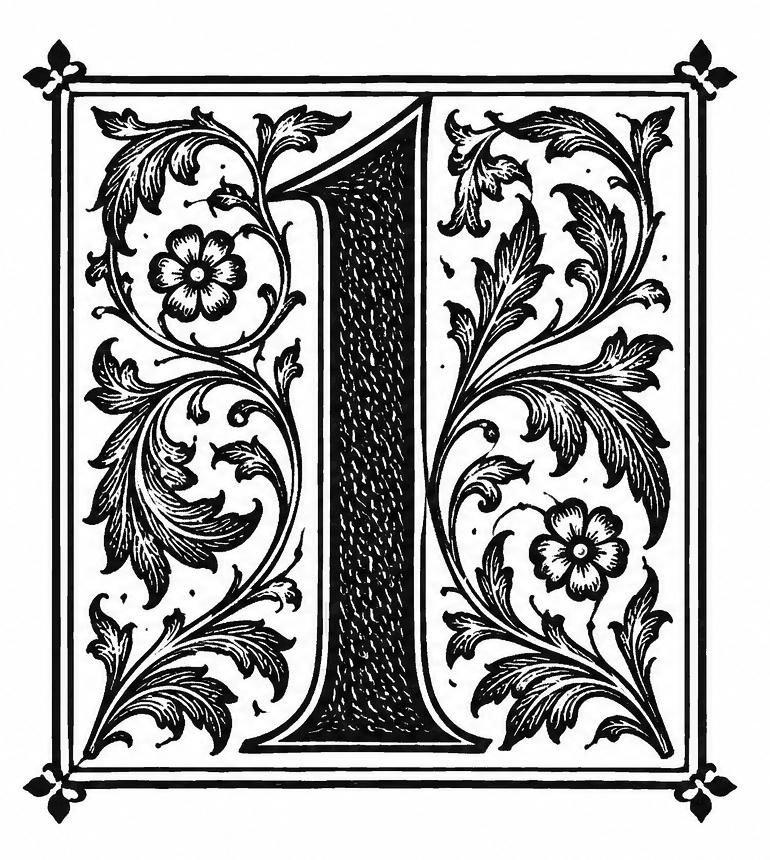
\includegraphics[width=2.5in]{drop_cap_1.png}
\caption{An ornamental numeral 1, the first appendix demonstration figure.}
\label{fig:app_numeral1}
\end{figure}

\begin{figure}
\centering
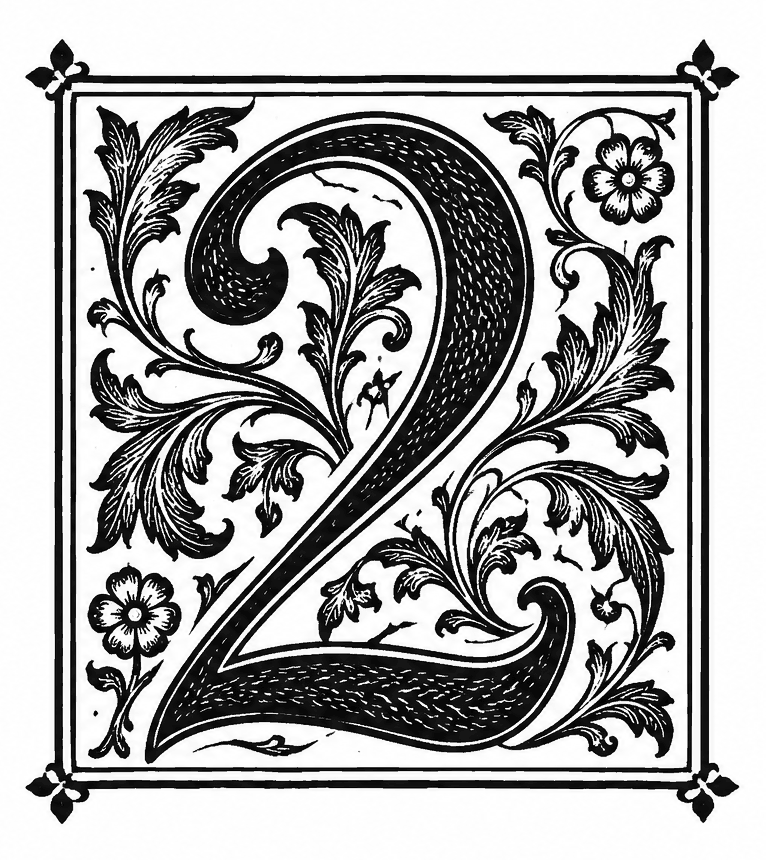
\includegraphics[width=2.5in]{drop_cap_2.png}
\caption{An ornamental numeral 2, the second appendix demonstration figure.}
\label{fig:app_numeral2}
\end{figure}

\section{Tables in an Appendix}

Here is an example of a table in an appendix showing how you might list websites you consulted. \cref{table:latexresources} lists free resources for learning \LaTeX\ and for answering questions as you write. The addresses are printed without the \texttt{https://} prefix, which keeps them short enough to fit the column, but each one still links to the full address:
\begin{verbatim}
\href{https://www.learnlatex.org}{\nolinkurl{www.learnlatex.org}}
\end{verbatim}
For an address printed in full, \verb+\url+ breaks long addresses at any character, thanks to the \texttt{xurl} package.

\begin{table}
\centering
\caption{Free Resources for Learning \LaTeX}
\label{table:latexresources}
\begin{tabularx}{\linewidth}{|>{\raggedright\arraybackslash}p{0.24\linewidth}|>{\raggedright\arraybackslash}p{0.36\linewidth}|>{\raggedright\arraybackslash}X|}
\hline
\textbf{Resource} & \textbf{Address} & \textbf{Good For} \\
\hline
Learn \LaTeX\ in 30 Minutes (Overleaf) & \href{https://www.overleaf.com/learn/latex/Learn_LaTeX_in_30_minutes}{\nolinkurl{www.overleaf.com/learn/latex/Learn_LaTeX_in_30_minutes}} & A first introduction, with examples you can edit online \\
\hline
learnlatex.org & \href{https://www.learnlatex.org}{\nolinkurl{www.learnlatex.org}} & Short interactive lessons covering the basics \\
\hline
Overleaf documentation & \href{https://www.overleaf.com/learn}{\nolinkurl{www.overleaf.com/learn}} & Task-based help on tables, figures, mathematics, and bibliographies \\
\hline
The Not So Short Introduction to \LaTeX & \href{https://ctan.org/pkg/lshort}{\nolinkurl{ctan.org/pkg/lshort}} & A complete free textbook \\
\hline
\LaTeX\ Wikibook & \href{https://en.wikibooks.org/wiki/LaTeX}{\nolinkurl{en.wikibooks.org/wiki/LaTeX}} & A searchable reference organized by topic \\
\hline
How Should We \LaTeX? (Roy Goodman) & \href{https://roygoodman.net/post/how-to-latex/}{\nolinkurl{roygoodman.net/post/how-to-latex}} & Style habits that manuals skip: meaningful macros, consistent notation, punctuating equations, and coauthoring \\
\hline
Short Math Guide for \LaTeX\ (AMS) & \href{https://ctan.org/pkg/short-math-guide}{\nolinkurl{ctan.org/pkg/short-math-guide}} & The commands of \texttt{amsmath} at a glance \\
\hline
Detexify & \href{https://detexify.kirelabs.org}{\nolinkurl{detexify.kirelabs.org}} & Finding the command for a symbol by drawing it \\
\hline
Comprehensive \LaTeX\ Symbol List & \href{https://ctan.org/pkg/comprehensive}{\nolinkurl{ctan.org/pkg/comprehensive}} & Every symbol available, with the package that provides it \\
\hline
TeX Stack Exchange & \href{https://tex.stackexchange.com}{\nolinkurl{tex.stackexchange.com}} & Answers to specific questions; search before asking \\
\hline
CTAN & \href{https://ctan.org}{\nolinkurl{ctan.org}} & Documentation for every package \\
\hline
\end{tabularx}
\end{table}

% \clearpage prints the floating Table A.1 first, so the tables stay in
% order; a longtable does not float and would otherwise come out first.
\clearpage
\section{Tables Longer Than One Page}

A table too long for one page is typed with the \texttt{longtable} environment instead of a \texttt{table} environment, as in \cref{table:longsample}. It does not float: it starts where it is typed and continues onto as many pages as it needs. Its title goes in the \verb+\endfirsthead+ part; the \verb+\endhead+ part, which starts with the class command \verb+\tablecontinued+, is repeated at the top of every later page, so each of them begins with ``\textbf{Table X.x (Continued)}'' and the column headings (GSO). The continued title is not listed again in the List of Tables.

\begin{longtable}{>{\centering\arraybackslash}p{0.15\linewidth}l>{\raggedright\arraybackslash}p{0.45\linewidth}}
\caption{Commands for Common Mathematical Symbols}
\label{table:longsample} \\
\toprule
\textbf{Symbol} & \textbf{Command} & \textbf{Meaning} \\
\midrule
\endfirsthead
\tablecontinued \\
\toprule
\textbf{Symbol} & \textbf{Command} & \textbf{Meaning} \\
\midrule
\endhead
\bottomrule
\endlastfoot
$\alpha$ & \verb+\alpha+ & Lowercase alpha \\
$\beta$ & \verb+\beta+ & Lowercase beta \\
$\gamma$ & \verb+\gamma+ & Lowercase gamma \\
$\delta$ & \verb+\delta+ & Lowercase delta \\
$\epsilon$ & \verb+\epsilon+ & Lowercase epsilon \\
$\zeta$ & \verb+\zeta+ & Lowercase zeta \\
$\eta$ & \verb+\eta+ & Lowercase eta \\
$\theta$ & \verb+\theta+ & Lowercase theta \\
$\iota$ & \verb+\iota+ & Lowercase iota \\
$\kappa$ & \verb+\kappa+ & Lowercase kappa \\
$\lambda$ & \verb+\lambda+ & Lowercase lambda \\
$\mu$ & \verb+\mu+ & Lowercase mu \\
$\nu$ & \verb+\nu+ & Lowercase nu \\
$\xi$ & \verb+\xi+ & Lowercase xi \\
$\pi$ & \verb+\pi+ & Lowercase pi \\
$\rho$ & \verb+\rho+ & Lowercase rho \\
$\sigma$ & \verb+\sigma+ & Lowercase sigma \\
$\tau$ & \verb+\tau+ & Lowercase tau \\
$\upsilon$ & \verb+\upsilon+ & Lowercase upsilon \\
$\phi$ & \verb+\phi+ & Lowercase phi \\
$\chi$ & \verb+\chi+ & Lowercase chi \\
$\psi$ & \verb+\psi+ & Lowercase psi \\
$\omega$ & \verb+\omega+ & Lowercase omega \\
$\varepsilon$ & \verb+\varepsilon+ & Variant of epsilon \\
$\vartheta$ & \verb+\vartheta+ & Variant of theta \\
$\varpi$ & \verb+\varpi+ & Variant of pi \\
$\varphi$ & \verb+\varphi+ & Variant of phi \\
$\Gamma$ & \verb+\Gamma+ & Uppercase gamma \\
$\Delta$ & \verb+\Delta+ & Uppercase delta \\
$\Theta$ & \verb+\Theta+ & Uppercase theta \\
$\Lambda$ & \verb+\Lambda+ & Uppercase lambda \\
$\Xi$ & \verb+\Xi+ & Uppercase xi \\
$\Pi$ & \verb+\Pi+ & Uppercase pi \\
$\Sigma$ & \verb+\Sigma+ & Uppercase sigma \\
$\Upsilon$ & \verb+\Upsilon+ & Uppercase upsilon \\
$\Phi$ & \verb+\Phi+ & Uppercase phi \\
$\Psi$ & \verb+\Psi+ & Uppercase psi \\
$\Omega$ & \verb+\Omega+ & Uppercase omega \\
$\nabla$ & \verb+\nabla+ & Gradient (nabla) \\
$\partial$ & \verb+\partial+ & Partial derivative \\
$\infty$ & \verb+\infty+ & Infinity \\
$\sum$ & \verb+\sum+ & Summation \\
$\prod$ & \verb+\prod+ & Product \\
$\int$ & \verb+\int+ & Integral \\
$\leq$ & \verb+\leq+ & Less than or equal to \\
$\geq$ & \verb+\geq+ & Greater than or equal to \\
$\neq$ & \verb+\neq+ & Not equal to \\
$\approx$ & \verb+\approx+ & Approximately equal to \\
$\in$ & \verb+\in+ & Element of \\
$\forall$ & \verb+\forall+ & For all \\
$\to$ & \verb+\to+ & Maps to, tends to \\
$\times$ & \verb+\times+ & Times, cross product \\
\end{longtable}



\end{document}